%% (Master) Thesis template
% Template version used: v1.4
%
% Largely adapted from Adrian Nievergelt's template for the ADPS
% (lecture notes) project.


%% We use the memoir class because it offers a many easy to use features.
\documentclass[11pt,a4paper,titlepage]{memoir}

%% Packages
%% ========

%% LaTeX Font encoding -- DO NOT CHANGE
\usepackage[OT1]{fontenc}

%% Babel provides support for languages.  'english' uses British
%% English hyphenation and text snippets like "Figure" and
%% "Theorem". Use the option 'ngerman' if your document is in German.
%% Use 'american' for American English.  Note that if you change this,
%% the next LaTeX run may show spurious errors.  Simply run it again.
%% If they persist, remove the .aux file and try again.
\usepackage[english]{babel}

%% Input encoding 'utf8'. In some cases you might need 'utf8x' for
%% extra symbols. Not all editors, especially on Windows, are UTF-8
%% capable, so you may want to use 'latin1' instead.
\usepackage[utf8]{inputenc}

%% This changes default fonts for both text and math mode to use Herman Zapfs
%% excellent Palatino font.  Do not change this.
\usepackage[sc]{mathpazo}

%% The AMS-LaTeX extensions for mathematical typesetting.  Do not
%% remove.
\usepackage{amsmath,amssymb,amsfonts,mathrsfs}

%% NTheorem is a reimplementation of the AMS Theorem package. This
%% will allow us to typeset theorems like examples, proofs and
%% similar.  Do not remove.
%% NOTE: Must be loaded AFTER amsmath, or the \qed placement will
%% break
\usepackage[amsmath,thmmarks]{ntheorem}

%% LaTeX' own graphics handling
\usepackage{graphicx}

%% We unfortunately need this for the Rules chapter.  Remove it
%% afterwards; or at least NEVER use its underlining features.
\usepackage{soul}

%% This allows you to add .pdf files. It is used to add the
%% declaration of originality.
\usepackage{pdfpages}

%% Some more packages that you may want to use.  Have a look at the
%% file, and consult the package docs for each.
%% See the TeXed file for more explanations

%% [OPT] Multi-rowed cells in tabulars
%\usepackage{multirow}

%% [REC] Intelligent cross reference package. This allows for nice
%% combined references that include the reference and a hint to where
%% to look for it.
\usepackage{varioref}

%% [OPT] Easily changeable quotes with \enquote{Text}
%\usepackage[german=swiss]{csquotes}

%% [REC] Format dates and time depending on locale
\usepackage{datetime}

%% [OPT] Provides a \cancel{} command to stroke through mathematics.
%\usepackage{cancel}

%% [NEED] This allows for additional typesetting tools in mathmode.
%% See its excellent documentation.
\usepackage{mathtools}

%% [ADV] Conditional commands
%\usepackage{ifthen}

%% [OPT] Manual large braces or other delimiters.
%\usepackage{bigdelim, bigstrut}

%% [REC] Alternate vector arrows. Use the command \vv{} to get scaled
%% vector arrows.
\usepackage[h]{esvect}

%% [NEED] Some extensions to tabulars and array environments.
\usepackage{array}

%% [OPT] Postscript support via pstricks graphics package. Very
%% diverse applications.
%\usepackage{pstricks,pst-all}

%% [?] This seems to allow us to define some additional counters.
%\usepackage{etex}

%% [ADV] XY-Pic to typeset some matrix-style graphics
%\usepackage[all]{xy}

%% [OPT] This is needed to generate an index at the end of the
%% document.
%\usepackage{makeidx}

%% [OPT] Fancy package for source code listings.  The template text
%% needs it for some LaTeX snippets; remove/adapt the \lstset when you
%% remove the template content.
\usepackage{listings}
\lstset{language=TeX,basicstyle={\normalfont\ttfamily}}

%% [REC] Fancy character protrusion.  Must be loaded after all fonts.
\usepackage[activate]{pdfcprot}

%% [REC] Nicer tables.  Read the excellent documentation.
\usepackage{booktabs}

\usepackage{caption}
\usepackage{subcaption}

%\usepackage{quotchap}
%\usepackage[utf8]{inputenc}


%% Our layout configuration.  DO NOT CHANGE.
%% Memoir layout setup

%% NOTE: You are strongly advised not to change any of them unless you
%% know what you are doing.  These settings strongly interact in the
%% final look of the document.

% Dependencies
\usepackage{ETHlogo}

% Turn extra space before chapter headings off.
\setlength{\beforechapskip}{0pt}

\nonzeroparskip
\parindent=0pt
\defaultlists

% Chapter style redefinition
\makeatletter

\if@twoside
  \pagestyle{Ruled}
  \copypagestyle{chapter}{Ruled}
\else
  \pagestyle{ruled}
  \copypagestyle{chapter}{ruled}
\fi
\makeoddhead{chapter}{}{}{}
\makeevenhead{chapter}{}{}{}
\makeheadrule{chapter}{\textwidth}{0pt}
\copypagestyle{abstract}{empty}

\makechapterstyle{bianchimod}{%
  \chapterstyle{default}
  \renewcommand*{\chapnamefont}{\normalfont\Large\sffamily}
  \renewcommand*{\chapnumfont}{\normalfont\Large\sffamily}
  \renewcommand*{\printchaptername}{%
    \chapnamefont\centering\@chapapp}
  \renewcommand*{\printchapternum}{\chapnumfont {\thechapter}}
  \renewcommand*{\chaptitlefont}{\normalfont\huge\sffamily}
  \renewcommand*{\printchaptertitle}[1]{%
    \hrule\vskip\onelineskip \centering \chaptitlefont\textbf{\vphantom{gyM}##1}\par}
  \renewcommand*{\afterchaptertitle}{\vskip\onelineskip \hrule\vskip
    \afterchapskip}
  \renewcommand*{\printchapternonum}{%
    \vphantom{\chapnumfont {9}}\afterchapternum}}

% Use the newly defined style
\chapterstyle{bianchimod}

\setsecheadstyle{\Large\bfseries\sffamily}
\setsubsecheadstyle{\large\bfseries\sffamily}
\setsubsubsecheadstyle{\bfseries\sffamily}
\setparaheadstyle{\normalsize\bfseries\sffamily}
\setsubparaheadstyle{\normalsize\itshape\sffamily}
\setsubparaindent{0pt}

% Set captions to a more separated style for clearness
\captionnamefont{\sffamily\bfseries\footnotesize}
\captiontitlefont{\sffamily\footnotesize}
\setlength{\intextsep}{16pt}
\setlength{\belowcaptionskip}{1pt}

% Set section and TOC numbering depth to subsection
\setsecnumdepth{subsection}
\settocdepth{subsection}

%% Titlepage adjustments
\pretitle{\vspace{0pt plus 0.7fill}\begin{center}\HUGE\sffamily\bfseries}
\posttitle{\end{center}\par}
\preauthor{\par\begin{center}\let\and\\\Large\sffamily}
\postauthor{\end{center}}
\predate{\par\begin{center}\Large\sffamily}
\postdate{\end{center}}

\def\@advisors{}
\newcommand{\advisors}[1]{\def\@advisors{#1}}
\def\@department{}
\newcommand{\department}[1]{\def\@department{#1}}
\def\@thesistype{}
\newcommand{\thesistype}[1]{\def\@thesistype{#1}}

\renewcommand{\maketitlehooka}{\noindent\ETHlogo[2in]}

\renewcommand{\maketitlehookb}{\vspace{1in}%
  \par\begin{center}\Large\sffamily\@thesistype\end{center}}

\renewcommand{\maketitlehookd}{%
  \vfill\par
  \begin{flushright}
    \sffamily
    \@advisors\par
    \@department, ETH Z\"urich
  \end{flushright}
}

\checkandfixthelayout

\setlength{\droptitle}{-48pt}

\makeatother

% This defines how theorems should look. Best leave as is.
\theoremstyle{plain}
\setlength\theorempostskipamount{0pt}

%%% Local Variables:
%%% mode: latex
%%% TeX-master: "thesis"
%%% End:


%% Theorem environments.  You will have to adapt this for a German
%% thesis.
%% Theorem-like environments

%% This can be changed according to language. You can comment out the ones you
%% don't need.

\numberwithin{equation}{chapter}

%% German theorems
%\newtheorem{satz}{Satz}[chapter]
%\newtheorem{beispiel}[satz]{Beispiel}
%\newtheorem{bemerkung}[satz]{Bemerkung}
%\newtheorem{korrolar}[satz]{Korrolar}
%\newtheorem{definition}[satz]{Definition}
%\newtheorem{lemma}[satz]{Lemma}
%\newtheorem{proposition}[satz]{Proposition}

%% English variants
\newtheorem{theorem}{Theorem}[chapter]
\newtheorem{example}[theorem]{Example}
\newtheorem{remark}[theorem]{Remark}
\newtheorem{corollary}[theorem]{Corollary}
\newtheorem{definition}[theorem]{Definition}
\newtheorem{lemma}[theorem]{Lemma}
\newtheorem{proposition}[theorem]{Proposition}

%% Proof environment with a small square as a "qed" symbol
\theoremstyle{nonumberplain}
\theorembodyfont{\normalfont}
\theoremsymbol{\ensuremath{\square}}
\newtheorem{proof}{Proof}
%\newtheorem{beweis}{Beweis}


%% Helpful macros.
%% Custom commands
%% ===============

%% Special characters for number sets, e.g. real or complex numbers.
\newcommand{\C}{\mathbb{C}}
\newcommand{\K}{\mathbb{K}}
\newcommand{\N}{\mathbb{N}}
\newcommand{\Q}{\mathbb{Q}}
\newcommand{\R}{\mathbb{R}}
\newcommand{\Z}{\mathbb{Z}}
\newcommand{\X}{\mathbb{X}}

%% Fixed/scaling delimiter examples (see mathtools documentation)
\DeclarePairedDelimiter\abs{\lvert}{\rvert}
\DeclarePairedDelimiter\norm{\lVert}{\rVert}

%% Use the alternative epsilon per default and define the old one as \oldepsilon
\let\oldepsilon\epsilon
\renewcommand{\epsilon}{\ensuremath\varepsilon}

%% Also set the alternate phi as default.
\let\oldphi\phi
\renewcommand{\phi}{\ensuremath{\varphi}}

\let\oldquote\quote
\let\endoldquote\endquote
\renewenvironment{quote}[2][]
{\if\relax\detokenize{#1}\relax
	\def\quoteauthor{#2}%
	\else
	\def\quoteauthor{#2~---~#1}%
	\fi
	\oldquote}
{\par\nobreak\smallskip\hfill(\quoteauthor)%
	\endoldquote\addvspace{\bigskipamount}}


%% Make document internal hyperlinks wherever possible. (TOC, references)
%% This MUST be loaded after varioref, which is loaded in 'extrapackages'
%% above.  We just load it last to be safe.
\usepackage[linkcolor=black,colorlinks=true,citecolor=black,filecolor=black]{hyperref}


%% Document information
%% ====================

\title{Group Key Managament for IoT networks}
\author{Ramy Chemak}
\thesistype{Master Thesis}
\advisors{Advisors: Dr. H. Lakhlef, Prof. A. Bouabdallah}
\department{Department of Computer Science}
\date{July 30, 2021}

\begin{document}

\frontmatter

%% Title page is autogenerated from document information above.  DO
%% NOT CHANGE.
\begin{titlingpage}
  %\calccentering{\unitlength}
  %\begin{adjustwidth*}{\unitlength-24pt}{-\unitlength-24pt}
  %  \maketitle
  %\end{adjustwidth*}
  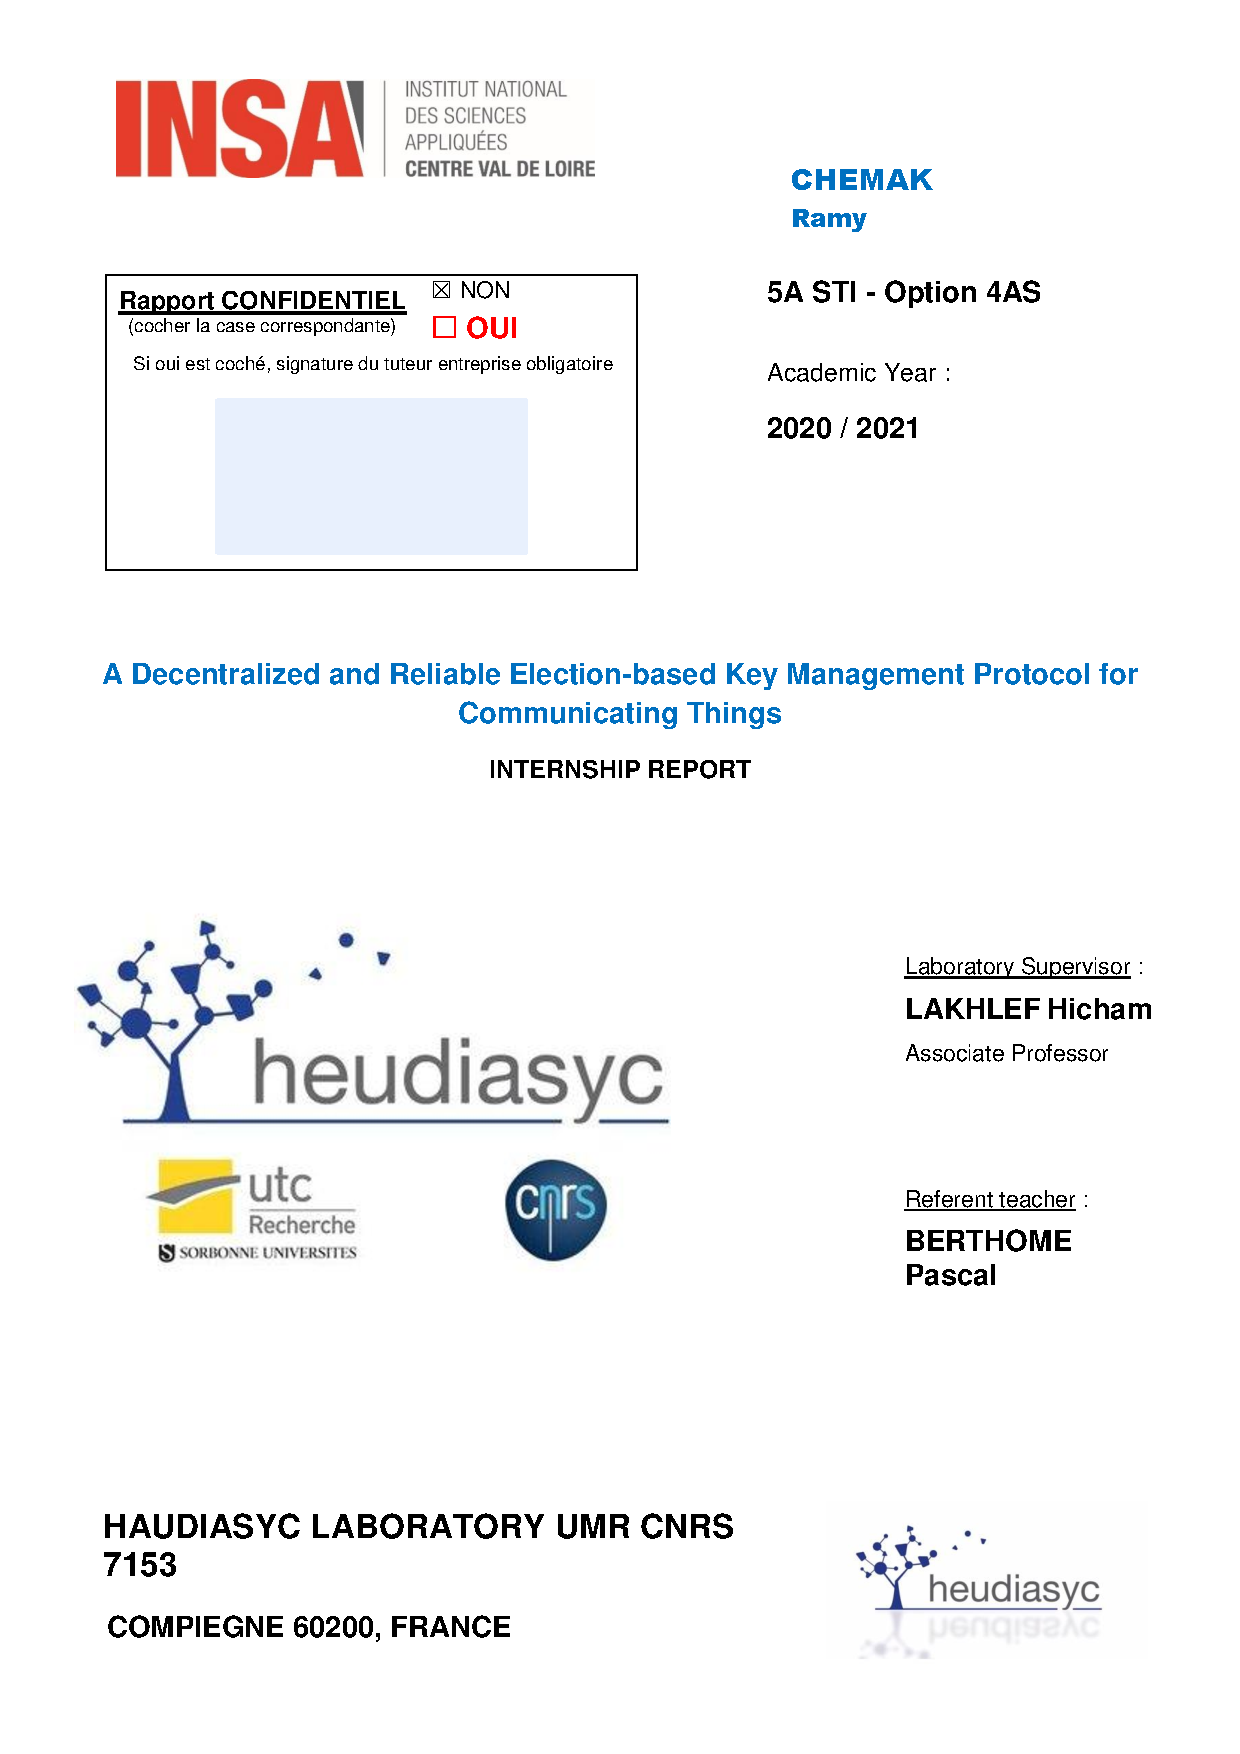
\includepdf[pages={-}]{cover.pdf}
\end{titlingpage}

%% The abstract of your thesis.  Edit the file as needed.
\chapter*{Acknowledgement}
%\addcontentsline{toc}{chapter}{Acknowledgement}

This report presents my work during this research internship. This would wouldn't have been achieved without the help of several people though.

I would first like to thank my referent teacher \textbf{Pr. Pascal BERTHOME} for his support and assistance with my application from the very start. The internship wouldn't have taken place without him.

I want also to thank my supervisors \textbf{Dr. Hicham LAKLHLEF} and \textbf{Pr. Abdelmadjid BOUABDALLAH} for offering me this opportunity. They provided me with their guidance and wise advice all along the internship.
\clearpage
\begin{abstract}
  Despite the large deployment of IoT devices during recent years, IoT networks privacy and security remains a major concern for users. With IoT networks reaching all aspects of our daily life, IoT security came under highlight more than ever.
  
  Researchers affiliated with the \emph{Heudiasyc laboratory UMR CNRS 7153} developed the Multi Group Key Management protocol (MGKMP), in order to ensure messages exchange security within IoT networks. This end-of-study internship is mainly a furtherance of previous research activities conducted at the host organization.
  
  The research internship main task was to further develop the MGKMP. In particular, it aims at solving issues related to the Key Manager (KM). A second minor task concerned working on IoT security as a practiced engineer rather than a researcher. These tasks were carried out with a certain level of success, and useful results could be produced.
  
  \textbf{Keywords:} Internet of Things (IoT), Key Management, energy, Cluster Head (CH), IoT security
\end{abstract}

\chapter*{Résumé}
%\addcontentsline{toc}{chapter}{Acknowledgement}

Malgré le déploiment à large échelle des réseaux IoT durant les dernières années, la sécurité de ces réseaux deumeurent encore un enjeu majeure. Plusieurs travaux de recherches menés et solutions proposées ont essayé de résoudre ce problème.

Une des solutions courantes repose sur le chiffrement des communications au sein de ces réseaux. Des chercheurs du laboratoire \emph{Heudiasyc laboratory UMR CNRS 7153} ont développé un protocole de gestion des clés cryptographiques pour les réseau IoT multi-groupes (MGKMP). L'objectif principal du stage est de continuer les recherches en cours au sein du laboratoire d'accueil.

La mission primaire du stage est de pousser le travail conduit sur MGKMP. En particulier, il était question d'aborder de plus près les problématiques liées au gestionnaire de clés. Une autre tâche secondaire consistait en l'étude de la sécurité IoT dans l'industrie en général. Les missions du stage ont été globalement accomplies avec un certain niveau de succès. En l'occurance, les travaux ont aboutit à des certains résultats plutôt satisfaisants.

\textbf{Mots clés:} Internet of Things (IoT), Gestion de clés cryptographiques, energie, Cluster Head (CH), sécurité IoT
%% TOC with the proper setup, do not change.
\cleartorecto
\tableofcontents
\clearpage
\listoffigures
\clearpage
\listoftables
%% Some commands used in this file
\newcommand{\package}{\emph}

\chapter*{Introduction}
\addcontentsline{toc}{chapter}{Introduction}

The use of Internet of Things (IoT) is continuously growing, and its application areas henceforth reach all societal and economical fields. IoT networks involve several applications such as smart agriculture, health care, smart homes ... etc. The number of connected IoT devices is increasing exponentially \cite{helpnet}, and so is the amount of their exchanged data. Some of these data might be sensitive or private. To ensure their security and integrity, encryption using Group Key Management (GKM) schemes were proposed. These schemes assume the presence of a centralized Key Manager (KM), which is regarded as the central component of the system.

Previous efforts by researchers affiliated with \emph{Heudiasyc laboratory UMR CNRS 7153} led to the development of the Multi Group Key Management protocol (MGKMP). The protocol already introduces a heap of new features and advantages. But number of its aspects are yet to be studied and improved. A part of the laboratory's work line is to to further push the research and development of MGKMP.

The internship splits into two main stages. The first stage is research oriented. Its mission is part of the laboratory's ongoing research activities on IoT security and GKM. As mentioned, it consists in the study of previous work done by the research team in charge, and elaborate upon it. The task was to study the MGKMP related issues deeper and try to adress them. Hence, the first stage was concluded with the publication of a research article in the proceedings of the \emph{International Conference on Communications Software (SoftCOM 2021)}.

The second stage was more oriented towards parctical engineering. The main objective was to acquire a solid culture in IoT security engineering in practice, and better apprehend the challenges involved.

The content of this report is organized as follows. Chapter~\ref{chap:litterature} reviews and discusses related academic works. Chapter~\ref{chap:mgkmp} studies the architecture of MGKMP and dig into some of its improvment axis. The main task dedicated to work the KM issue of single point of failure out is presented in Chapter~\ref{chap:key_manager}. This includes the problematic definition (Section~\ref{sec:km_problem}), solution design (Section~\ref{sec:election-based-scheme}), simulations and results evaluation (Section~\ref{sec:simulations_results}). Finally, Chapter~\ref{chap:iot_security} sums the second stage up, mainly studying different aspects of IoT security engineering.

%\mainmatter
%\backmatter
%% Some commands used in this file
\newcommand{\package}{\emph}

\chapter*{Introduction}
\addcontentsline{toc}{chapter}{Introduction}

The use of Internet of Things (IoT) is continuously growing, and its application areas henceforth reach all societal and economical fields. IoT networks involve several applications such as smart agriculture, health care, smart homes ... etc. The number of connected IoT devices is increasing exponentially \cite{helpnet}, and so is the amount of their exchanged data. Some of these data might be sensitive or private. To ensure their security and integrity, encryption using Group Key Management (GKM) schemes were proposed. These schemes assume the presence of a centralized Key Manager (KM), which is regarded as the central component of the system.

Previous efforts by researchers affiliated with \emph{Heudiasyc laboratory UMR CNRS 7153} led to the development of the Multi Group Key Management protocol (MGKMP). The protocol already introduces a heap of new features and advantages. But number of its aspects are yet to be studied and improved. A part of the laboratory's work line is to to further push the research and development of MGKMP.

The internship splits into two main stages. The first stage is research oriented. Its mission is part of the laboratory's ongoing research activities on IoT security and GKM. As mentioned, it consists in the study of previous work done by the research team in charge, and elaborate upon it. The task was to study the MGKMP related issues deeper and try to adress them. Hence, the first stage was concluded with the publication of a research article in the proceedings of the \emph{International Conference on Communications Software (SoftCOM 2021)}.

The second stage was more oriented towards parctical engineering. The main objective was to acquire a solid culture in IoT security engineering in practice, and better apprehend the challenges involved.

The content of this report is organized as follows. Chapter~\ref{chap:litterature} reviews and discusses related academic works. Chapter~\ref{chap:mgkmp} studies the architecture of MGKMP and dig into some of its improvment axis. The main task dedicated to work the KM issue of single point of failure out is presented in Chapter~\ref{chap:key_manager}. This includes the problematic definition (Section~\ref{sec:km_problem}), solution design (Section~\ref{sec:election-based-scheme}), simulations and results evaluation (Section~\ref{sec:simulations_results}). Finally, Chapter~\ref{chap:iot_security} sums the second stage up, mainly studying different aspects of IoT security engineering.

\mainmatter

%% Your real content!
%% Some commands used in this file
\newcommand{\package}{\emph}

\chapter{Introduction}

This is version \verb-v1.4- of the template.

We assume that you found this template on our institute's website, so
we do not repeat everything stated there.  Consult the website again
for pointers to further reading about \LaTeX{}.  This chapter only
gives a brief overview of the files you are looking at.

\section{Features}
\label{sec:features}

The rest of this document shows off a few features of the template
files.  Look at the source code to see which macros we used!

The template is divided into \TeX{} files as follows:
\begin{enumerate}
\item \texttt{thesis.tex} is the main file.
\item \texttt{extrapackages.tex} holds extra package includes.
\item \texttt{layoutsetup.tex} defines the style used in this document.
\item \texttt{theoremsetup.tex} declares the theorem-like environments.
\item \texttt{macrosetup.tex} defines extra macros that you may find
  useful.
\item \texttt{introduction.tex} contains this text.
\item \texttt{sections.tex} is a quick demo of each sectioning level
  available.
\item \texttt{refs.bib} is an example bibliography file.  You can use
  Bib\TeX{} to quote references.  For example, read
  \cite{bringhurst1996ets} if you can get a hold of it.
\end{enumerate}


\subsection{Extra package includes}

The file \texttt{extrapackages.tex} lists some packages that usually
come in handy.  Simply have a look at the source code.  We have
added the following comments based on our experiences:
\begin{description}
\item[REC] This package is recommended.
\item[OPT] This package is optional.  It usually solves a specific
  problem in a clever way.
\item[ADV] This package is for the advanced user, but solves a problem
  frequent enough that we mention it. Consult the package's
  documentation.
\end{description}

As a small example, here is a reference to the Section \emph{Features}
typeset with the recommended \package{varioref} package:
\begin{quote}
  See Section~\vref{sec:features}.
\end{quote}


\subsection{Layout setup}

This defines the overall look of the document -- for example, it
changes the chapter and section heading appearance.  We consider this
a `do not touch' area.  Take a look at the excellent \emph{Memoir}
documentation before changing it.

In fact, take a look at the excellent \emph{Memoir} documentation,
full stop.


\subsection{Theorem setup}

This file defines a bunch of theorem-like environments.

\begin{theorem}
  An example theorem.
\end{theorem}

\begin{proof}
  Proof text goes here.
\end{proof}

Note that the q.e.d.\ symbol moves to the correct place automatically
if you end the proof with an \texttt{enumerate} or
\texttt{displaymath}.  You do not need to use \verb-\qedhere- as with
\package{amsthm}.

\begin{theorem}[Some Famous Guy]
  Another example theorem.
\end{theorem}

\begin{proof}
  This proof
  \begin{enumerate}
  \item ends in an enumerate.
  \end{enumerate}
\end{proof}

\begin{proposition}
  Note that all theorem-like environments are by default numbered on
  the same counter.
\end{proposition}

\begin{proof}
  This proof ends in a display like so:
  \begin{displaymath}
    f(x) = x^2.
  \end{displaymath}
\end{proof}


\subsection{Macro setup}

For now the macro setup only shows how to define some basic macros,
and how to use a neat feature of the \package{mathtools} package:
\begin{displaymath}
  \abs{a}, \quad \abs*{\frac{a}{b}}, \quad \abs[\big]{\frac{a}{b}}.
\end{displaymath}

% Some commands used in this file
\newcommand{\package}{\emph}

\chapter*{Introduction}
\addcontentsline{toc}{chapter}{Introduction}

The use of Internet of Things (IoT) is continuously growing, and its application areas henceforth reach all societal and economical fields. IoT networks involve several applications such as smart agriculture, health care, smart homes ... etc. The number of connected IoT devices is increasing exponentially \cite{helpnet}, and so is the amount of their exchanged data. Some of these data might be sensitive or private. To ensure their security and integrity, encryption using Group Key Management (GKM) schemes were proposed. These schemes assume the presence of a centralized Key Manager (KM), which is regarded as the central component of the system.

Previous efforts by researchers affiliated with \emph{Heudiasyc laboratory UMR CNRS 7153} led to the development of the Multi Group Key Management protocol (MGKMP). The protocol already introduces a heap of new features and advantages. But number of its aspects are yet to be studied and improved. A part of the laboratory's work line is to to further push the research and development of MGKMP.

The internship splits into two main stages. The first stage is research oriented. Its mission is part of the laboratory's ongoing research activities on IoT security and GKM. As mentioned, it consists in the study of previous work done by the research team in charge, and elaborate upon it. The task was to study the MGKMP related issues deeper and try to adress them. Hence, the first stage was concluded with the publication of a research article in the proceedings of the \emph{International Conference on Communications Software (SoftCOM 2021)}.

The second stage was more oriented towards parctical engineering. The main objective was to acquire a solid culture in IoT security engineering in practice, and better apprehend the challenges involved.

The content of this report is organized as follows. Chapter~\ref{chap:litterature} reviews and discusses related academic works. Chapter~\ref{chap:mgkmp} studies the architecture of MGKMP and dig into some of its improvment axis. The main task dedicated to work the KM issue of single point of failure out is presented in Chapter~\ref{chap:key_manager}. This includes the problematic definition (Section~\ref{sec:km_problem}), solution design (Section~\ref{sec:election-based-scheme}), simulations and results evaluation (Section~\ref{sec:simulations_results}). Finally, Chapter~\ref{chap:iot_security} sums the second stage up, mainly studying different aspects of IoT security engineering.
\chapter{Literature Review}
\label{chap:litterature}

\section{Related work}

\subsection{Group Key Management}

\subsubsection{Mathematical approach}

GKM as a problematic has several dimensions and different types of issues to consider and tackle. Some research focused on reliable key generation issues in GKM. In \cite{zhan_novel_2017}, the authors analyzed the impact of key management techniques on connectivity and efficiency in Wireless Sensor Networks (WSNs). In order to address the issue, they propose a key generation method based on system of equations. Considering how the work was carried out to tackle poor connectivity and multiple forwarding issues, the solution is actually pretty scalable. The paper considers a system of u equations with v variables as follows:

\begin{math}
	\Phi^{\left(v\right)} =
	\left\{
	\begin{array}{l}
		\phi_1 \left(x_1, x_2, \ldots, x_v\right) = 0\\
		\vdots \\
		\phi_u \left(x_1, x_2, \ldots, x_v\right) = 0
	\end{array}
	\right.
\end{math}\\

This equation has one unique solution which will be used to generate a shared secret key to be shared among the network’s nodes. Solutions of equation systems actually constitute the associated keys, from which we then generate those secret keys. Two systems of equations were considered: linear equations and polynomial equations. The first system was recommended over the second one, due to its lower complexity.

Another solution based on the Kronecker product was proposed in \cite{tsai_key_2017}. Authors of the paper already proposed CRAPPY (Constrained RAndom Perturbation-based Pairwise keY establishment), a key establishment protocol for WSNs. However the latter doesn’t consider heterogeneity in IoT networks, neither scalability related issues. Considering the exponential growth of IoT devices and their diversity, this protocol is simply impractical. The authors utilize the matrix Kronecker product to generate private and public keys for the network’s nodes. We cite the property:

\begin{quote}
	\begin{math}
		If\; A \in \mathcal{R}^{\sqrt{m} \times \sqrt{m}} \; and\; A \in \mathcal{R}^{\sqrt{n} \times \sqrt{n}} \; are\; symmetric,\; then\; A \otimes G\; is\; symmetric. 
	\end{math}
%If $A \mathcal{R}^{\sqrt{m}\times\sqrt{m}}$ and $A \mathcal{R}^{\sqrt{n}\times\sqrt{n}}$ are symetric, then $A\otimesG$ is symetric. 
\end{quote}

Therefore, we are able to generate couples of keys for each of the network’s nodes. The system assigns a couple of keys, private and public, to each node. The paper more in depth how the system exactly works. Its resilience resides in the difficulty of reconstructing the Kronecker product by any of the sensor nodes. Besides, it factorizes asymmetric encryption for messages exchange, which is rather safer than symmetric encryption.

\subsubsection{Key management architectures}

Tiloca and Dini in \cite{tiloca_grep_2016} proposed GREP, a group rekeying protocol. The protocol assumes the presence of an IDS. The latter’s main function is to detect eventual attacks on the network, in order to identify compromised nodes to be evicted. However, the paper points out that nodes suspected by the IDS as compromised are considered unreliable, and therefore will also be evicted by the Group Membership Service. Thus, each node compromising or suspicion will probably induce the whole rekeying upon leaving process.
Yet this topic is not covered in the paper. Even though it’s beyond the scope the treated problematic, the service role in the overall problem seems under-valued. Actually, the quality of the IDS can significantly influence the global efficiency reference criteria of the rekeying protocol. On one side, a well-designed IDS is able to efficiently detect which nodes exactly are compromised. As suspected nodes are also to be evicted, the IDS can eventually raise some false alarms. Hence, optimising the IDS accuracy will decrease the number of possible false alarms, and so the number of useless rekeying process operations with all the cost that comes with. On the other side, some attack scenarios involve compromising one node at first, before propagating in the network reaching others. If the IDS is efficient enough to provide early detection of compromised nodes, it can lower the rekeying process’ cost which should follow. Regarding the rekeying upon leaving process detailed in the paper, having few compromised nodes belonging to a limited number of subgroups is clearly an advantage.
So we can see here that IDS role can be crucial in the key management protocol, as it can significantly contribute in the saving of the network’s bandwidth and limiting the node’s energy drainage.

The rekeying process, whether upon a joining node or a leaving one, is based on one central element which is the refreshing key $K_R$. The latter is then employed in order to generate almost all new tokens and encryption keys for group, subgroup and pairwise communications. However, the paper doesn’t explain precisely how this $K_R$ is generated, nor the measures taken to secure its generation.

Kung and Hsiao \cite{kung_groupit_2018} proposed GroupIt, a two-tier GKM architecture. It supports multi-group networks, and embeds its own methodologies to handle device membership updates. The upper tier is resposible for key management between different groups. The lower tier is however responsible for key management within groups. The architecture considers two types of groups: device groups and user groups. Device groups incorporate devices based on their technical functionalities and security requirements. The systems also establishes user groups which contain one or multiple device groups. A device group can belong to different user groups, and every user is assigned to one and only one user group.

\begin{figure}[htbp]
	\centerline{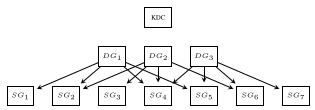
\includegraphics[scale=0.75]{figures/groupit.png}}
	\caption{Source \cite{kung_groupit_2018}: GroupIt initial structure overview}
	\label{groupit}
\end{figure}

Every device group has its own GKM scheme, such as Logical Key Hierarchy (LKH). But above all these groups, we have a KDC which provides keys for inter-group communications. Although the proposed system considers mechanisms to ensure secure communications, forward and backward secrecy, and resistance against collusion attacks, it still has a central problem: the whole lies on the KDC. This centralization generates a single point of failure within the architecture. That’s why we need to dig deeper into decentralization issues and proposed solutions.

\subsubsection{Decentralized key management}
\label{subsec:decentralized}

Several solutions for decentralized Key Management were considered. Veltri et al. \cite{veltri_novel_2013} proposed a batch-based group key management. The solution looked more at distributing the rekeying operations as events. The protocol relies on a central Key Distribution Center though, so the key management as a role remains centralized after all. Dammak et al. \cite{dammak_decentralized_2020} proposed a decentralized Group Key Management architecture. This hierarchical architecture relies on several Key Distribution Centers (SKDCs) with a central Key Distribution Center (KDC) on top. This solution already distributes the task of key management, but only partially. The SKDCs aren’t completely autonomous regarding the KDC and are still dependant on it. Hence, the issue of single point of failure persists. The Blockchain technology was also considered \cite{truong_towards_2019, kouicem_decentralized_2019} to address the problem. The use of Blockchain requires from every node to keep its own copy of the ledger. This solution takes us from a point where a single entity is handling the key management, to a situation where practically all network nodes are acting as Key Manager. Giving the need to add a ledger block on every rekeying operation, this introduces a significant processing overhead (due to required Proof-of-Works) and networking overhead (due to required ledger update).

A cluster based Key Management solution was suggested by Khan and Anandharaj in \cite{feroz_khan_cognitive_2019}. It uses a cognitive key management technique to increase energy efficiency and scalability. The work considers Cluster Head (CH) election process and highlights the need for cluster maintenance. However, the proposed election process adopts a classical network routing approach. Besides, it does not consider security risks related to this cluster based scheme, nor its mitigation. The algorithm’s analysis is focused on energy efficiency, with few regard to security.

\subsection{Cluster Head selection}
\label{subsec:ch}

Actually, Cluster Head based architectures have been long studied. Heinzelman et al. \cite{heinzelman_energy-efcient_2000} considered network clustering as a network routing solution. They proposed LEACH (Low-Energy Adaptive Clustering Hierarchy) to address the energy dissipation issue in node-to-base station communications. It suggests a cluster-divided network with one node in every cluster acting as local Base Station (BS), dubbed CH. Different CHs collect data from their fellow cluster members, and transmit them to the main BS. Extensions of this scheme were then proposed \cite{al-baz_new_2018, kang_distance_2012}. Other algorithms for CH selection seeking to optimise energy consumption and load-balancing were suggested in \cite{behera_residual_2019, jia_dynamic_2016}. These algorithms utilize node’s energy capabilities to balance probabilities for CH selection among other cluster nodes. But all these studies aim to optimise energy performances with no regard to security. They were basically developed to save radio transmission overhead, thereby they deal with network and data routing oriented problems. However, our interest for this scheme is foremost driven by our need to solve the Key Management problem for group communication and provide a decentralized model for it. Moreover, the CH election in previous works is based on energy, communication and networking related criteria. Besides, they mainly consider homogeneous environments in which CH are to communicate with a fixed Base Station (BS) for application reasons. Hence, the described models are not necessarily fit for use as a security oriented scheme (cryptographic key management in our case) for heterogeneous IoT networks. In our use case, we tend more to think over the architecture from a security point of view.

\section{Identification of remaining challenges}

In literature review, we considered both, decentralized key management as a challenge and network clustering as a scheme. Based upon this, we can notice that these works are mostly energy performance oriented. We need key management and cryptographic keys to ensure security in the first place. Despite that the main problematic, key management, is actually a security problematic, relevant researches are usually conducted with a networking and energy mindset, sometimes discarding security concerns \cite{ziegeldorf_privacy_2014, zhang_iot_2014, khan_iot_2018}. This work aims at bringing back the security perspective to the front view, besides the energy aspect. Thus to propose a solution which offers a satisfactory security-efficiency compromise.
\chapter{Multi Group Key Management Protocol}
\label{chap:mgkmp}

The main mission of the internship is to continue the underway research work on the Multi Group Key Management Protocol (MGKMP), being conducted within the host lab. Section~\ref{sec:mgkmp_overview} presents key elements the work done so far. It's kind of a literature review specific to the lab's scientific production. The rest of this chapter sums up the first assignment, which consists in the in-depth study of the protocol and identification of work yet to be done.

\section{Overview of MGKMP}
\label{sec:mgkmp_overview}

The MGKMP is organized in three layers. The first layer is intended for node and key management. Each node is assigned to a subgroup $S^i_j$ of the group $G_i$. Managed keys can be categorized into Data Encryption Keys (DEKs) and Key Encryption Keys (KEKs). These keys are either used for device-to-device communications (pairwise keys) or group and subgroup communications. The second layer is intended for subgroup management. This partitioning considerably decreases the nodes' storage overhead. The third and last layer is intended for service and group management. Groups are chosen according to a unique combination of services. Fig.~\ref{fig:mgkmp_layers} illustrates the MGKMP architecture. Still to note that subgroups layer is logical and totally transparent to the application layer.

\begin{figure}[htbp]
	\centerline{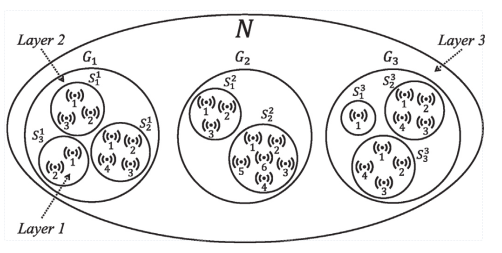
\includegraphics[scale=0.60]{figures/mgkmp/mgkmp_layers.png}}
	\caption{Source \cite{kandi_versatile_2020}: Example of a network partitioning}
	\label{fig:mgkmp_layers}
\end{figure}

The protocol aims at ensuring five different properties: scalability, efficiency, heterogeneity, collusion resistance and forward and backward secrecy. The two last properties are security oriented, whereas the first three ones are used to evaluate the protocol's performance. Forward secrecy is guaranteed when a leaving member of a group has no longer access to his former group communications. Backward secrecy is guaranteed when a joining member of a group has no access to his group's old communications. A collusion attack unfolds when multiple compromised nodes (evited or not) cooperate using their individual pieces of information to gain illegitimate access to the group key. To curb these security risks, the protocol relies on keys revokes and rekeying operations. Every time a node is joining, leaving or evicted from a group, all pairwise keys associated with these node as well as related group keys are revoked and new ones are generated. Rekeying operations and group memberships are handled by the Key Manager (KM). This makes the KM the protocol's security backbone.

Among key contributions of MGKMP is its compatibility with heterogeneous networks. Giving the increasingly sophisticated and inter-connected nature of IoT networks, this is a major asset.

\section{Optimization of MGKMP}
\label{sec:mgkmp_optimization}

These working tracks consider mainly the optimzsation of the MGKMP protocol. The idea consists in redesigning some aspects of the protocols features, and then comparing the new design’s complexity and other properties with the original design. Presumably, each optimization brought should be compared apart, and eventually, a combination of those could be tested. The ultimate objective is to produce a better optimized version of MGKMP in terms of security, resilience, flexibility, efficiency and scalability.

\subsection{Analysis of an n-tier architecture}
\label{subsec:n-tier}

The first subgroup layer in the paper aims at grouping devices by physical capacity and power. Thereby, it decreases energy drainage for devices. But this extra layer piles up complexity to the overall architecture and cryptographic key management, whether those used for group or device-to-device communications. This complexity increase shadows on the raising number of required messages during rekeying operations, and therefore, an increase in network traffic and bandwidth consumption. However, network traffic indulged on a network adapter is itself a factor of energy drainage for the device.

Now let’s imagine an extension of the suggested protocol to a 4-tier architecture. This might contribute to the enhancement of the storage overhead and computation effort for a device node. But it would probably lead to ever further utilization of network bandwidth as well, and so, the device battery might waste on network adapters what it had saved from its CPU. However, the study of both aspects of the protocol’s performance shall lead to a proper compromise.

\begin{figure}[htbp]
	\centerline{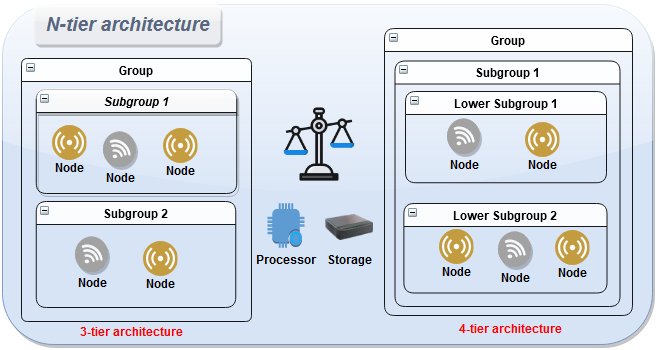
\includegraphics[scale=0.60]{figures/mgkmp/n-tier.png}}
	\caption{3-tier architecture vs. 4-tier architecture}
	\label{fig:n-tier}
\end{figure}

A naive question to sum up the issue would be:

\begin{quote}
	\emph{What consumes more energy: network adapters or CPUs ?}
\end{quote}

It is agreed upon though that network adapters consume more energy than processors. Since we are considering heterogeneous IoT networks, the devices we are facing can be very much different. Therefore, it’s going to be difficult to say which physical component is more likely subject for optimisation and energy saving enhancement. Therefore, this task will most likely requires an overview and  analysis of common devices’ physical capacities in order to compare with the analysis of bandwidth and CPU utilization influence on energy drainage. The study is not to be necessarily restricted for the computation and network capacity. Other elements might interfere in the carried out process, and so they are to be taken into account as well.

Similarly to the Storage Capability Evaluation Function, we can define for instance a look-alike function for the Network Capability Evaluation Function. Hence, the ultimate Capacity, according which nodes are attributed to subgroups, will be the average of these two functions. The average does not have to be static though. It can very well be dynamic according to the device’s physical characteristics, and common patterns can be defined for this purpose. In case of a successful theoretical analysis, implementing an experimental prototype for a real-life use case shall make perfect sense.

The work on this axe of optimisation can contribute significantly to the scalability and efficiency of of the proposed solution.

\subsection{Re-order algorithm upon leave}
\label{subsec:re-order}

In the aftermath of a node’s exit out of the network, a rekying process upon leave in launched by the Key Manager. In case a subgroup’s cardinal decreases down to a certain threshold, then it’s merged with an other subgroup. Concretely, the solution looks for an subgroup to merge with, creates a new subgroup to which it assigns the nodes from the two merging subgroups, and finally removes the latter two subgroups.

Sometimes this merge process comes after the eviction of a compromised node, in which case the two merging subgroups could be compromised. In this situation, and for security reasons, it’s rather pertinent to have them both removed and create a new one with freshly generated keys. Nevertheless, this is not always the case. When no security breach requires it, this would only be a waste of computational power and bandwidth and loss of efficiency.

\begin{figure}[htbp]
	\centerline{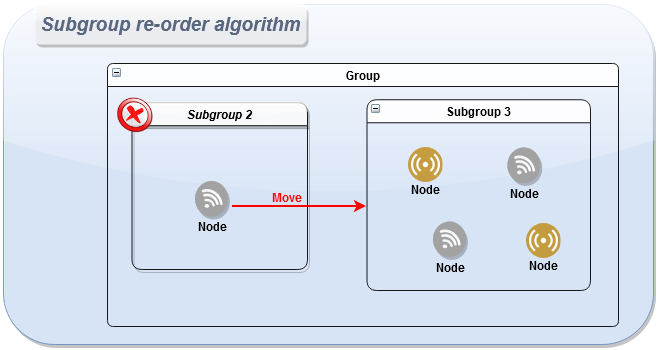
\includegraphics[scale=0.60]{figures/mgkmp/reorder.png}}
	\caption{MGKMP subgroup's re-order algorithm}
	\label{fig:re-order}
\end{figure}

A simple example to illustrate the kind of optimisation to bring on, is when a subgroup $S_1$ of cardinal $n=2$ is to merge with another subgroup $S_2$ of cardinal $n=8$, assuming we have a threshold $thr=2$. In this case, it would rather much more efficient to just assign the nodes from $S_1$ to $S_2$ and provide them with the necessary keys, instead of creating a new subgroup $S_3$. In this case, the 8 initial nodes from $S_2$ are saving all the computational power required for key generation as well as bandwidth for message exchanges for joining the of $S_3$. These 8 nodes have practically nothing to do. Moreover, the KM would have saved the computational energy for the creation of $S_3$, and its key generation.

\subsection{Sub-grouping sequences}
\label{subsec:subgroups}

As mentioned previously, layer 2 is intended for subgroup management. Nodes within a group are subdivided into multiple subgroups based on their minimal capabilities $mc$.This $mc$ value is determined through two main algorithms, referred as sequences: powers of two and Fibonacci.

\begin{figure}[htbp]
	\centerline{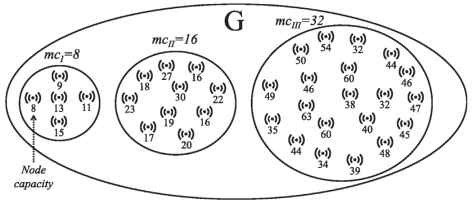
\includegraphics[scale=0.60]{figures/mgkmp/power2.png}}
	\caption{Source \cite{kandi_versatile_2020}: Example of a group partitioned using powers of 2 sequence}
	\label{fig:power2}
\end{figure}

This subgrouping sequences could be studied further, in order to eventually develop new efficient sequencing algorithms.

\section{Internal liabilities of MGKMP}
\label{sec:mgkmp_liabilities}

The corresponding working tracks seek to enhance the protocol’s security by looking into its performance when applied into practice. Many features of the protocol are demonstrated in a abstract and theoretical way. But some of the slightest behaviours in their concrete implementations might turn out to be extremely costy. Some of these features interact with each other, which can have implications on how they should be defined for practical implementation. The hereby considered problematic also deals with efficiency enhancement as well as security enforcement. So the point is to look out how practical the theoretical definitions of MGKMP are, and how to adjust eventual inconveniences.

\subsection{Refresh key generation}
\label{subsec:random_gen}

\begin{quote}{\emph{Robert R. Coveyou}}
	The generation of random numbers is too important
to be left to chance.
\end{quote}

%\begin{savequote}[45mm]
%	The generation of random numbers is too important
%to be left to chance.
%	\qauthor{Robert R. Coveyou}
%\end{savequote}

One of MGKMP's key properties is forward and backward. The main mechanism implemented to ensure it is the group rekeying process. As described in Section~\ref{sec:mgkmp_overview}, the new key is generated via a KDF which takes the old key and a random key $K_R$ as parameters. From a cryprographic point of view, the random generation is crucial to the whole process. Any vulnerability can blow the forward and backward secrecy up. An evicted or leaving node already has the old key. So if it gets hold of $K_R$, it can easily compute the new key. A recently joined node already has the new key. So if it gets hold of $K_R$, it will be possible to deduce the old one.

\begin{figure}[htbp]
	\centerline{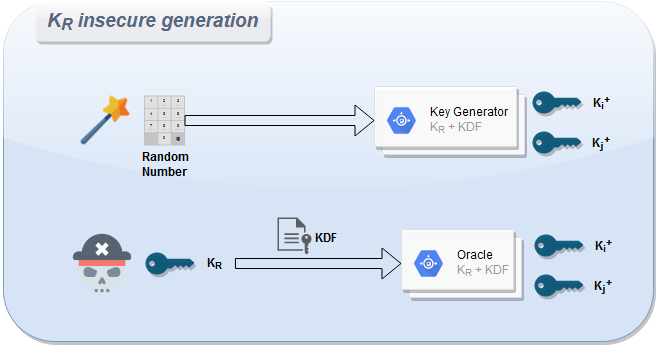
\includegraphics[scale=0.60]{figures/mgkmp/random.png}}
	\caption{Insecure $K_R$ generation}
	\label{fig:random_gen}
\end{figure}

Fig.~\ref{fig:random_gen} illustrates how an attacker who is able to guess $K_R$ and knows the KDF used, is able to compute newly generated secret keys by using some cryptographic oracle.

\subsection{Node's join authorization \& pre-secure channel}
\label{subsec:node_join}

The joining of a new node comes with two assumptions. First, the joining node is reliable and trustworthy. And the second implies that we dispose of a pre-existing secure channel between the Key Manager and and the joining node.
The first assumption don’t take into consideration the possibility that a node can already be compromised before it joining the network. Therefore, it burdens the risk of having all the new node’s keys systematically compromised.
The second assumption assumes the communication’s security between the Key Manager before having the node’s join process through. The non-compromising of all encryption keys related to the new node depends on this channel’s resilience.
In both cases above, we have a systematic key compromising situation just in the aftermath of a node’s join operation. This will eventually lead to have this node evicted afterwards, and hence, launching a rekeying upon leaving process.

\begin{figure}[htbp]
	\centerline{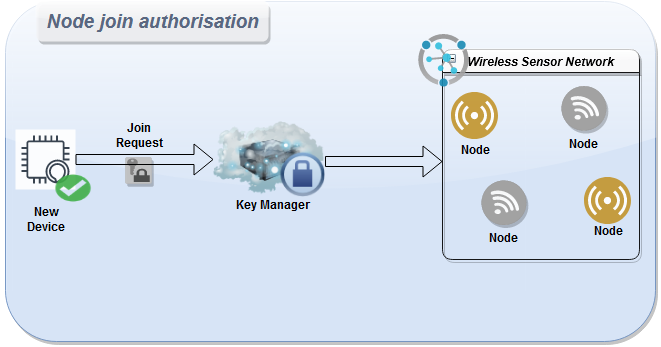
\includegraphics[scale=0.60]{figures/mgkmp/join_auth.png}}
	\caption{Node's join authorization}
	\label{fig:node_join}
\end{figure}

\subsection{Inadequate choice for cryptographic algorithms}
\label{subsec:cryptography}

Depending on the data to hash or encrypt, algorithms have to be considered with caution. It's easy to mistake cryptographic algorithms for an independant and irrelevant problem in our case. But MGKMP is protocol which directly deals with cryptography. When we look at common cryptographic issues, they are more related to the system implementation, rather than the algorithm itself. Although the algorithm's choice remains beyond the scope of this research work, it has to be thought in advance to facilitate the enginneer's work, who is actually implementing MGKMP. The point of this section is to underline the influence of protocol's design in hardening or easing the resilience of implemented cryptographic algorithms. It doesn't assume any lack or flaw in the protocol, such conclusion can only be the outcome of a dedicated study.

\subsubsection{Insecure key exchange}

Key exchange protocols solve a crucial problem, which is sharing a secret key between two communicating entities over an insecure channel. The most widely used protocol today is Diffie-Hellman. It can be implemented using discrete logarithms and elliptic curves. Even though the protocol is mathematically resilient, it's absolutely helpless against Man-in-the-Middle MITM attacks.

\subsubsection{Insecure hash functions}

Hash functions are very used in the MGKMP, but they have to be consiered carefully. Hash algorithms like MD5 or SHA-1 are utterly broken. SHA-2 hash family is more performant and safer than SHA-1, for its collision resistance. But once again, depending on the context, attacks like reduced-round collisions \cite{chowdhury_new_2008} or length extension attacks aren't excluded.

\subsubsection{Message authentication codes}

In relation with Section~\ref{subsec:node_join}, the use of Message Authentication Codes (MAC) is almost unavoidable. But that's a cryptographic challenge itself \cite{debian} and requires robust design of the related feature in MGKMP. For instance, prefix-MAC constructions is totally insecure even with SHA-2. Only SHA-3 algorithms allow the implementation of safe MAC systems.

\subsubsection{Signature algorithms}

The most robust signature algorithms available actually rely on public key cryptography. Attacks on RSA such as common modulus, hasted attack, Wiener's attack or common factor attack are leathal. How trustworthy asymmetric cryptography can be, it still has its own weaknesses. What is interesting is that these flaws aren't related to the crypto-system itself, but to its implementation. This means that these vulnerabilities should be carefully considered when designing a security system based on cryptography, as it's the case here.

\subsubsection{Lightweight cryptography algorithms}

Once more, the system designed here directly concerns cryptography. The resource-constraint nature of the IoT rather drives the attention towards lightweight cryptography algorithms \cite{bhardwaj_review_2017, surendran_survey_2018}. The choice of these algorithms has to take into account context requirements, since their characteristics differ according to the use case \cite{muthavhine_analysis_2018}. But something recurrent in these lightweight algorithms, is the curb of their resilience in favor of performance gain. This can be for example round reduction in AES algorithms, or the use of easy-to-generate initialization vectors (IV) in stream ciphers. If the host system (the MGKMP architecture in our case) allows it, such measures can lead to related-key attacks on AES \cite{hutchison_key_2010, hutchison_related-key_2009} or IV attacks on CBC and ECB.

\section{Analysis of the protocol's ecosystem}
\label{sec:ecosystem}

\begin{quote}{\emph{Pete Herzog --- The Open Source Cybersecurity Playbook}}
	The first key to any effective security game plan in knowing what you’re up against
\end{quote}

So far, the protocol’s related research work focused mainly on the conception the protocol’s processes and the exclusive definition of its internal core functionalities. In many cases, the development undertook a mathematical approach to identify different problems and solve them. However, the protocol shall be integrated in a probably complex environment, where its own functioning will influence and be influenced by external actors and components. This protocol already solve several critical security issues and significantly decrease the probability of an IoT network’s compromise. However, it’s only an actor in a bigger interconnected and hostile ecosystem.

This section seeks to provide some ideas for the analysis of these interactions, measurement of their impact on the well-functioning of the protocol, and suggestions to improve the protocol considering the conducted risk analysis. The point is to see the problematic from different angles in order to better apprehend the protocol’s ecosystem and the stakes which come along, in order to have a system practically compatible with any or at least most common environments seen in major use cases. Furthermore, some aspects of the protocol could be possibly enhanced in order to cover up for attack vectors coming from those actors and reduce the attack surface.

The previous threats and vulnerabilities enumeration demonstrate some of the possible attack vectors for cryptographic key compromising. Since our protocol aims mainly at securing cryptographic key exchange and encrypting data transmission, then these attack scenarios could of interest for study. In these examples, we demonstrate that an attacker does not necessarily have to break the protocol’s design itself in order to compromise the managed cryptographic keys. But he can however look for actors in the overall ecosystem interacting with our protocol, and take advantage of its eventual weaknesses.

The protocol’s environment to consider is pretty large and can include a variety of inter-connected actors interacting with our nodes and the Key Manager. Tiloca and Dini \cite{tiloca_grep_2016} already described an architecture in which the KM performs its duties. This architecture involves a Key Management System (KMS) operating above the KM. On the same level as the KMS, we have a Group Membership Service (GMS) keeping track of which nodes belong to the group. In our architecture, we can very intuitively imagine that this same service would also be keeping track of which nodes membership regarding subgroups as well. When a new node joins in or is evicted out of the group, the GMS should have a process to carry out in order update its membership lists. Still on the same level as the KMS, the architecture includes an Intrusion Detection Service (IDS), assuming the task of identifying malicious nodes and report them the GMS to have them evicted. Finally, on top of the three services (GMS, KMS and IDS), we have a group controller (GC), which role is to oversee the well functioning of these services. Fig.~\ref{fig:grep} illustrates the architecture described by the authors of the GREP protocol.

\begin{figure}[htbp]
	\centerline{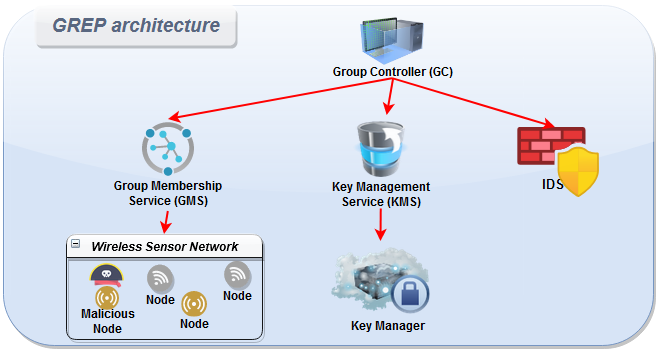
\includegraphics[scale=0.60]{figures/mgkmp/grep.png}}
	\caption{GREP architecture}
	\label{fig:grep}
\end{figure}

However, a realistic infrastructure in which the Key Management protocol shall be integrated is definitely much more sophisticated that the one described above. Fig.~\ref{fig:ecosystem} illustrates, in a non-exhaustive way, the diversity and complex interconnection of a realistic environment. We can see below the Key Manager and the Wireless Sensor Network which are embedded in the core of the protocol. But all around we have a dynamic and active ecosystem of several entities interacting with both. Among those entities, we have a firewall, through which go all transmissions from and to the group. There is as well the GMS and an IDS, as already discussed. In order to mitigate risks of a malicious node joining the group, we can imagine an Identity Access Management system in order to check out a node’s join request legitimacy. This IAM service can also assume other responsibilities in our environment. The IAM service, depending on the use case, can be substituted with an Access Control Server (ACS). As it’s more and more common, we can assume that our network is somehow related to some Cloud-based service. Therefore, additional security constraints are also to be considered by the protocol. Furthermore, the node’s architecture itself is an element worth attention, whether form a software or a hardware point of view. Further features such as logs generation by the KM for eventual forensics analysis can be considered too.

\begin{figure}[htbp]
	\centerline{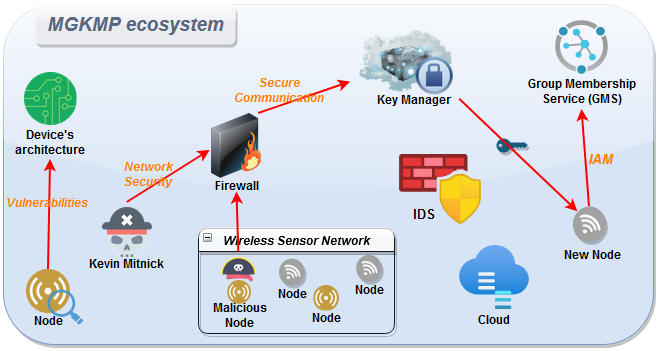
\includegraphics[scale=0.60]{figures/mgkmp/ecosystem.png}}
	\caption{Key Management protocol's ecosystem}
	\label{fig:ecosystem}
\end{figure}

From previous analysis, a number of attacks such as the low-level Sybil attack and RPL routing attacks are actually conducted by malicious nodes within the network. Our protocol doesn’t interfere in the detection process of veiled nodes. But it does make sure, throughout the rekeying upon leave process, that this node is indeed evicted and cannot access the network’s communications afterwards, ie. ensures forward secrecy.

Firewalls are a central element in IoT networks in order to filter out unnecessary or malicious network frames originally destined for some node, especially with the ever coming-back energy constraints. Yet, firewalls are also an attractive concentration point of network traffic. The compromise of the firewall, even partially through a foothold, might to the compromise of other nodes, if not the whole network. That’s why communications going through in and out should all be enough secured and authenticated, at risk of jeopardizing internal communications on the group. Among other reasons, this can significantly mitigate risks of insecure neighbor attacks. The device-to-device communications requires a prior steps of router discovery and address resolution. A firewall in the inside can make sure that these messages aren’t detoured to a malicious destination. The firewall can also be deployed to monitor these internal communications themselves, in which case node-to-node and KM-to-node messages will all go through the firewall. If the network’s security is not robust enough, a hacker would be able to eavesdrop on some communications allowing more damaging attacks such as fragmentation replay and duplication attack or just tampering with frames. The latter is actually a very serious threat as it opens the door for a bit-flipping attack.

The protocol is essentially designed to ensure cryptographic keys management and exchange between different nodes and the KM. As briefly explained above, the network’s infrastructure can sometimes be easily eavesdropped on. This ease in intercepting transmissions might very well allow an attacker to measure and analyse time required for nodes to perform protocol related encryption operation, exposing the protocol to a category of side-channel attacks, known as Timing attacks. This also intercross with the previously part mentioning the Timing attack.

In Section~\ref{subsec:node_join}, we discussed the problematic of the pre-established secure channel between the KM and new joining node. A reliable communication over this channel requires an end-to-end security on the transport layer. The purpose is to make ensure reception of a message by the desired destination while authenticating the sender. Here we go back to Message Authentication Codes (MAC) and message signature algorithms, already discussed in Section~\ref{subsec:cryptography}. This measure concerns joining nodes as well as device-to-device communications. Device-to-device communications should also bare the network security aspect since they are subject to session establishment and resumption attacks. These attacks can badly affect the integrity of, among others, some Data Encryption Keys (DEKs).

To quickly sum up the previous, we have a recurring problem, which is node compromising. It’s here where the importance of malicious node detection stands out. For this point, we already assumed the likely presence of an IDS in our ecosystem. We have also considered a firewall filtering internal communications of the group, in which case it can also monitor the network traffic in the same time to detect abnormal behaviours. An independent monitoring solution, such as a Zabbix server, could be considered too, while its output can be used for veiled activities detection. Depending on which solution is to be used, we need to make sure that different operations carried out by the Key Management will always be compatible with its environment. We can even consider different versions of the protocol for each use case, with eventual optimisations for each facilitating the bad nodes hunt. All of this requires a standalone study and analysis to select what can possibly be done on this path.

Besides, all previously mentioned entities such as IAM service, firewalls and ACS are actively interacting with the group nodes and the KM, as already mentioned. To some extent, and depending on the situation, some on them could even be considered as insider actors of the group communication. Hence, they are technically members of the group, requiring encryption keys provided by the KM on their turn. As a consequence, an other study and analysis could be carried out to precise (i) which keys exactly these elements will need to efficiently assume their functions, (ii) how are they going to be distributed by the KM and also regarding the other nodes, and foremost (iii) how the KM should handle them and manage their keys. This study shall improve the implementability of the protocol and make it easier to integrate in a concrete industrial application.

Finally, the Key Management protocol already takes into consideration different characteristics of IoT devices, such as their low computation power or constrained energy capacity. Those considered characteristics are mainly physical though. There is much more in the devices to be studied in order to analyse its implication of well functioning of the protocol. In case of popping up issues, optimisations and improvement shall be made on the protocol’s design to make it further operational. This study turns around the devices systems, from the hardware as well as the software point of view.

On the software level, we have already mentioned some typical threats including malwares. A malware-infected node can easily have all its stored encryption keys compromised. To this purpose, we can think of some security mechanisms regarding how keys are to be stored on the device. These mechanisms have already been thought in the protocol, but only regarding the storage overhead. So a further study of this part can very well enhance the integrity of the protocol.
From the hardware point of view, two main elements should be considered to assess the protocol’s efficiency and usability in its environment: (i) the device’s firmware and (ii) the processor’s architecture. The hardware study is crucial as it allows the assessment of the risk level regarding a possible rootkit compromising. Same as for malwares, a rootkit infected node can easily have all of  its encryption keys compromised. Nevertheless, rootkits are far more lethal than high level malwares and foremost, they are extremely stealthy and hard to detect, if they are detectable. Rootkits raise the interest of studying the processor’s architecture besides the firmware. The interest in considering processors architectures could come from other threats too, like the Timing attack. An analysis can conclude on whether the protocol’s key exchange and storage processes take this kind of threat into account or not, then conclude on which enhancements, if possible, can be added to make the protocol more resilient.
\chapter{Key Manager: Single Point of Failure}
\label{chap:key_manager}

In Chapter~\ref{chap:mgkmp}, we described a number of issues related to the MGKMP, without going deeper or proposing solutions. One more issue concerns the Key Managar (KM). For the latter, we decided we would be working more in depth on it, and propose a solution to solve the problem. This Chapter represent the internship's main mission, which led to the article publication.

\section{Problem description}
\label{sec:km_problem}

The whole architecture of the proposed solution above lays on one central component: the Key Manager. This vital component is to handle on its own the complete key management infrastructure and all the processes defined in the protocol, such as the rekeying process or key generation. Since we are considering a multi-group scheme, each group is handled by a Key Manager.

The Key Manager has to permanently satisfy the three main security properties: Confidentiality, Integrity and Availability (CIA). Any failure or the compromising of this machine will systematically jeopardise the whole security infrastructure of the group. A security breach of the KM can have devastating consequences, leading to the leak of the stored encryption keys used by respective group fellows.

A typical scenario is when the KM is down. This could be due to some malfunctioning in the system, or even a cyber-attack like a DDoS attack, or just result from some overload submitted to the KM, since it coordinates all nodes in the network. It could also occur upon an incident like a blaze in a datacenter \cite{malwarebytes}. In this situation, no rekeying process is going to be possible, as this operation is on the KM’s responsibility. Therefore if a compromised node is detected, either by neighbouring nodes or by a third party defense system like an IDS, it won’t be possible to have it evicted from the group. It wouldn’t be possible to have the group tided up neither. Basically, whatever device has detected the compromising, it would automatically report it to the KM in order to have it settled. However, since the KM is down, this eviction request will never be treated, and the cleaning up operation will never be carried out. Moreover, as long as the KM remains down, the compromised node will remain a member of the group having all group’s communication it’s allowed to compromised. Furthermore, the node not being evicted once it’s uncovered, it can spread into the network compromising all group related keys it hasn’t yet in its inventory.

\begin{figure}[htbp]
	\centerline{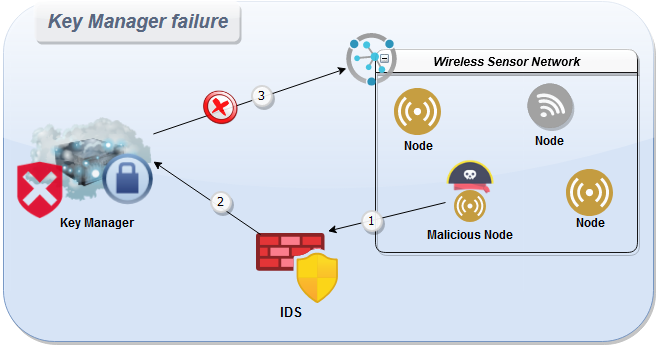
\includegraphics[scale=0.55]{figures/mgkmp/failure.png}}
	\caption{Key Manager failure scenario}
	\label{fig:km_failure}
\end{figure}

One would want to say that if we add some redundancy to the KM, that would solve the problem. If the main KM is down, then we have some backup clones to take over until the main one is on track again. Nevertheless, this isn’t necessarily guaranteed, because availability isn’t the only security requirement to satisfy as mentioned above. To illustrate this, we can imagine an interference in the communications from and to the KM. A malicious node or a third party attacker can spoof the KM’s identity and hence, conduct a Man in the Middle (MITM) attack. If the KM is compromised, then so are all operations it is carrying out and the infrastructure as a whole would be rotten to the core. Even if the communications are encrypted, the attacker can still tamper with a rekeying process upon a node’s leave. Actually, if the attacker has access to the leaving node’s keys, then he can forge rekying messages with the old revoked keys. That way it would be as the whole rekeying operation hasn’t took place, and the leaving node will have a theoretically unauthorised access to so many communications, making them all compromised. An attacker acting like a proxy for the KM can also intercept messages for a joining node. But as a pre-secure channel should be established between the KM and the new node, the way he can compromise these messages depends on how this channel is implemented.

This attack is a bit more difficult than the previous to mount though, since the attacker has to manipulate data (eg. the ARP table) for every node and other entity that might be in interaction with the KM. Unless the KM is placed behind a single component, such as a Firewall, then the attack difficulty would depend on the resilience of the latter.

\begin{figure}[htbp]
	\centerline{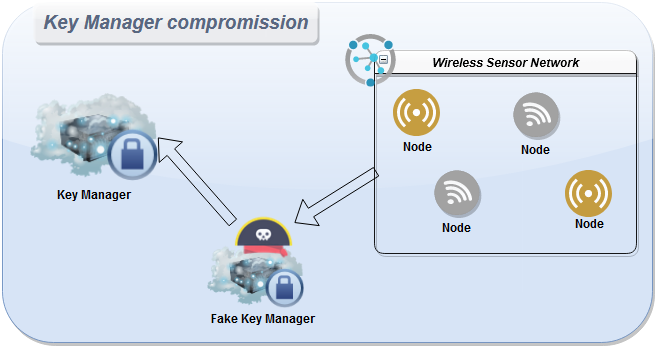
\includegraphics[scale=0.55]{figures/mgkmp/comprom.png}}
	\caption{Key Manager compromising scenario}
	\label{fig:km_mitm}
\end{figure}

To sum up, we have two main problems concerning this architecture making out of the KM a single point of failure. The first one concerns the load imposed over the KM. It has to coordinate every node from groups and subgroups. Every join or leave operation is validated by the KM, and the consequent rekeying operations are also handled by it. In the original design, we already assume that the KM is powerful and robust. But such performance assumptions can be costy, and still, it remains a system with its own physical limits like any other system. All this makes the KM a \textbf{\textit{single point of charge}}. Second, we also make the assumption that the KM is trustworthy. The fact that all network membership evolution have to be validated by the KM, and the rekeying process is entirely handled by it as well, gives it a large base of trust. The MITM attack described above shows how critical this trust can be. This makes the KM a \textbf{\textit{single point of trust}}. A way to mitigate these risks, is to design a decentralised architecture with a distributed base of trust and a distributed load of charge.

\section{Blockchain-based scheme}

Kandi et al. \cite{kandi_lightweight_nodate} suggested a solution based on the Blockchain technology as explained previously (see Chapter~\ref{chap:litterature}). This solution however might end up too costy for IoT networks. One one side, the Blockchain implies that all nodes, regardless of their storage capacity, will have to store the ledger, which will definitely cause a significant additional storage overhead. The more traffic we have (nodes joining and leaving), the more blocks have to be added. This makes the storage overhead, in addition to its height, dynamic and of an unpredictable growth. Moreover, these transactions will introduce a consequent network traffic. Hence, an increase in bandwidth consumption and drainage of node’s already-constrained resources. Besides the performance hindering, a hacker can see in this an opportunity to conduct a parallel DoS attack. By maliciously interfering with the network traffic, one can instigate false join and leave requests, which will be translated into appended blocks to the ledger. Abusing this kind of interference might consume the total node’s storage capacity. On the other side, each block append to the ledger requires a computational effort, a Proof of Work. PoW operations or even PoS operations in the Blockchain aren’t the most trivial to compute. They require a certain minimum threshold of computational power, and the way the Blockchain technology was designed in the first place, tend to have such threshold as high as possible, which is exactly what we want to avoid. Even with some lightweight versions of the Blockchain, it doesn’t resolve entirely the problem and it may very well add further problems. Those lightweight versions are actually based on constraint-reduced PoW or PoS. However, this can open the door for some security risks since transactions would be easier to validate, and so the vote process will be more accessible. Hence, malicious nodes will be more likely to conduct veiled activities, and we’re not even sure if the computational capacity problem is solved.

\section{Election-based scheme}
\label{sec:election-based-scheme}

Another strategy for distributed charge and trust for the Key Manager, is to have an election-based scheme, where any node can be the KM. This way, we mitigate the risk of single point of failure present in the original design on one hand. And on the other hand, we don’t necessarily have all nodes assuming the costy role of a KM like in a Blockchain-based scheme. The main idea is that one node among the group will assume the responsibility of a KM (which is already possible in the centralised version). This node has been chosen and approved by the others. This choice is based on some node-related technical criteria, which make it eligible for this role. In case the KM down or compromised, any other eligible node can take over. A KM can also choose, if the situation allows and requires it, to hand over its responsibilities in case it is or will be suffocating. The KM still uniquely assumes the responsibility of the key generation process during a rekeying operation, but it can share the burden of newly generated keys distribution with the others. In this scheme, key generation has also been improved and optimised for less energy drainage. In addition to the role of a KM, we also define a deputy, which is the privileged node to take over if the KM is, for some reason, deemed to step down. This deputy has also a monitoring role over the KM.

\begin{figure}[htbp]
	\centerline{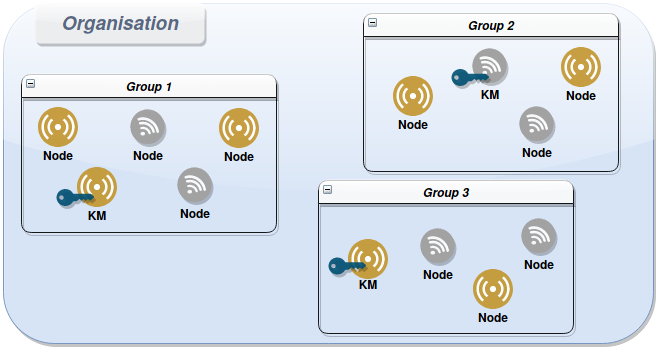
\includegraphics[scale=0.50]{figures/organisation.png}}
	\caption{Election-based scheme architecture}
	\label{fig}
\end{figure}

In Section 1.1.2, we discussed several Cluster Head (CH) selection algorithms. However, these algorithms were mostly designed to address network routing and data exchange problems, such as LEACH (Low-Energy Adaptive Clustering Hierarchy) \cite{heinzelman_energy-efcient_2000} and related extensions \cite{al-baz_new_2018, kang_distance_2012}. Other algorithms for CH selection seeking to optimise energy load-balancing were  proposed in \cite{behera_residual_2019, jia_dynamic_2016}. These algorithms utilizes node’s energy capabilities to balance probabilities for CH selection among other cluster nodes. But all these studies aim to optimise energy performances with no regard to security. They were basically developed to save radio transmission overhead, thereby they deal with network and data routing oriented problems. However, our interest for this scheme is foremost driven by our need to solve the Key Management problem for group communication and provide a decentralised model for it. Moreover, the CH election in previous works is based on energy, communication and networking related criteria. Besides, they mainly consider homogeneous environments in which CH are to communicate with a fixed Base Station (BS) for application reasons. Hence, the described models are not necessarily adapted for use as a security oriented scheme (cryptographic key management in our case) for heterogeneous IoT networks. In our use case, we tend more to think over the architecture from a security point of view. The main security criterion the CH must satisfy is availability. We are not using the CH a as relay between nodes and some BS. We are rather building a security infrastructure to manage cryptographic keys in order to secure both group and device-to-device communications between different nodes. When rethinking the election-based scheme from this prospective, we actually end up with many additional constraints than those already considered.

\begin{figure}[htbp]
	\centerline{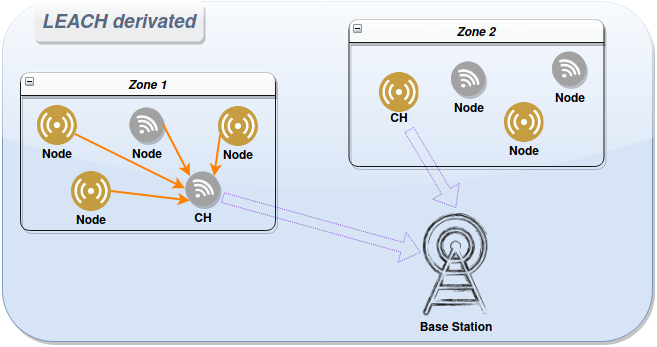
\includegraphics[scale=0.50]{figures/LEACH.png}}
	\caption{Overview of LEACH-based architecture}
	\label{fig}
\end{figure}

In this section, we propose a new complete election-based scheme adapted for Key Management in multi-group IoT networks. The point is to successfully define a decentralised election-based infrastructure for Key Management which (i) solves the problem of KM single point of failure, (ii) satisfies the heterogeneous and energy-constraint nature of IoT networks, (iii) considers the main objectives we target from a security point of view, and (iv) tries to inherit as possible the features offered by previous work (even thought not all of those are needed for our use case).
In the very first basic approach, the idea was to have one unique component that handles the Key Management, where came the problem of single point of failure from. In the first attempt to solve the problem, the Blockchain technology was considered, where the energy consumption problem came from. So we basically went from having one single node doing this heavy important task in the first case, to a state where all nodes are assuming this role regardless of their capabilities in the second case. The approach we would like to propose tries to combine both previously mentioned approaches in order to suggest something in between. The advantage of the election-based approach is that it have one particularly capable node acting as KM (the first approach likewise) while actually allowing any node in the network to take part (the second approach likewise). The fact that this node will be elected and validated guarantees the reliability of the KM from both security and performance point of view. Therefore, the architecture should support decentralised decision making, and thus enhance failure management. As for the KM election, it should take into consideration security concerns through consensus-based trust. Finally, to maintain scalability and IoT performance requirements, the architecture must be flexible and involve minimum vote processes and communication overhead.

\subsection{Technical eligibility criteria}

Basically, any node can be the KM and that’s the basis to have a distributed system. However, those can be heavy and expensive responsibilities to assume, which require minimum capacities in networking, storage and processing. Otherwise the node could be merely qualified as single point of failure by default. To ensure that a candidate node will be up to it when qualifying for KM, we define two new functions: Processing Capacity Evaluation Function (PCEF) and Networking Capacity Evaluation Function (NCEF). Those two new functions will be aggregated with the already defined Storage Capacity Evaluation Function (SCEF) as an input for the Capacity Evaluation Function (CEF). The latter's output is what gives us the bigger picture about the node’s real technical capabilities and qualification for the KM’s assignments. The output of the CEF is a score, which has to be above a minimum threshold for a node to be eligible for the role of the KM. The final score value shall be correlated with the node’s energetic capacities as well. This settled, we ensure that an elected node for KM is indeed technically and energetically reliable.

The CEF score should be an average value totally blinding regarding the input values. For this purpose, the input values could, eventually, be aggregated with a salt to add some noise. There are two main reasons why the CEF’s output is a single dark value. The first reason is saving network bandwidth and energy. In this form, a node will be just broadcasting a number, instead of a long message detailing its capacities. Besides, this increases accuracy when providing a reference scale for decision making (voting). The second one is security related. One is never sure whether a pre-compromised node is present in the group like a Trojan horse, or an outsider attacker is somehow eavesdropping on the group communications. Therefore, it’s more secure if the CEF score doesn’t leak any data about a node’s real capabilities in networking, storage and processing. The acquisition of such information can be used to mount other specific attacks, and so very harmful. A typical example, is side channel attacks in cryptanalysis. Knowledge of some physical properties of a device can significantly increase the efficiency of these category of attacks, in a context where cryptographic choices are critical (see Section 3.4).

\begin{figure}[htbp]
	\centerline{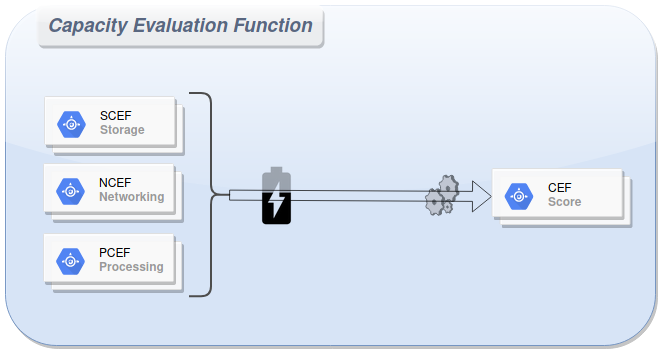
\includegraphics[scale=0.50]{figures/cef.png}}
	\caption{Capacity Evaluation Function score}
	\label{fig}
\end{figure}

\subsubsection{Technical description of CEF score}

The CEF score is computed based upon three inputs SCEF, PCEF and NCEF correlated with an energy score.

First of all, we start with the SCEF since it’s already at our disposal. The KM, as its name suggests, will have to manage keys. Among other things, it stores all cryptographic keys used to secure communications within the group, as each group has an independent KM, and exchanges with other groups. The larger the group is, the more related keys the KM will have to manage. Thus, the KM must have some some storage capabilities, especially if we want to preserve the scalability which can involve numerous group fellows. The SCEF was defined in \cite{kandi_versatile_2020} by:

\begin{equation}\label{eq1}
	c_k = pm \; .\; \frac{sc_k}{ks}
\end{equation}

where
\begin{math}
	\left\{
	\begin{array}{l}
		s_k: storage\; capacity\; of\; a\; node\; u_k\\
		sc_k: storage\; capability\; of\; a\; node\; u_k\\
		pm: usable\; percentage\; of\; memory\; by\; protocol\\
		ks: size\; of\; a\; key
	\end{array}
	\right.
\end{math}\\

For conformity issues, we bring slight edit to the notations above, thus redefining the SCEF as:

\begin{equation}\label{eq2}
	s_k = pm \; .\; \frac{sc_k}{ks}
\end{equation}

\begin{math}
s_k:\; storage\; capacity\; of\; a\; node\; u_k
\end{math}

The rest of notations are maintained.

The next step is the definition of PCEF. The PCEF is a function we introduce in order to assess the processing capacities of the node, a potential KM candidate. Actually, all group related keys are exclusively generated by the KM. But a key generation involves the execution of cryptographic functions, which are by default expensive in terms of processing. As discussed in Section~\ref{sec:mgkmp_liabilities}, lowering the standards of cryptographic systems implementation may degrade its reliability. Thereby, enough processing capacities are crucial to maintain a high resilience level of the protocol. In Section 5.1.1 of \cite{kandi_versatile_2020} related to the theoretical analysis of the overheads of the KM, we cite:

\begin{quote}
	Property 2: Calculation overhead on the KM is proportional to the sum $p+m_j$.
\end{quote}

Based upon this property, we define the PCEF score as follow:
\begin{equation}\label{eq2}
	p_k = pp \; .\; \frac{cc_k}{cs \; .\; \left( p + m_j \right)}
\end{equation}

where
\begin{math}
	\left\{
	\begin{array}{l}
		p_k: processing\; capacity\; of\; a\; node\; u_k\\
		cc_k: computation\; capability\; of\; a\; nod\;e u_k\\
		pp: usable\; percentage\; of\; processor\; by\; protocol\\
		cs: overhead\; of\; crypto\; system\\
		p: number\; of\; subgroups\; of\; the\; group\; G\\
		m_j: number\; of\; nodes\; in\; subgroup\; S_j
	\end{array}
	\right.
\end{math}\\

The above definition of pk takes very well into consideration the fact that the KM will handle exchange security between other groups and his own, during different rekeying operations, according to the rekeying procedure defined in MGKMP. The function considers the percentage of processing the protocol can use. This means that nodes which processing units are perfectly designed to only handle their application related tasks, such as some wireless sensors, won’t be very favorable as KM candidate. The computation capability $cc$ is a static value based on physical characteristics of a device (eg. the processing unit’s frequency in Mhz).

The last of the three capacity criteria to consider is the NCEF. Rekeying operations, as defined in MGKMP, involve big time communication overhead for the KM, from joining messages to leaving messages. Besides, theses messages are transmitted in all possible fashions: unicast, multicast or broadcast. Moreover, for a newly joining node, the first communication channel is to be established with the KM in order to proceed with the join (see Section~\ref{subsec:node_join}). This channel has to be robust from a networking point of view, and shall not be hindered by low networking capabilities. As mentioned, rekeying operations might require the KM communicating with other groups, eventually physically far distanced, which even highlights further the importance of communication range and strength of the KM candidate. Even if the node is selected as supplicant KM, it will have the task of monitoring the main KM, which involves way a lot of networking. The deputy KM has to be ready to assume functions of an active KM at anytime anyway. In Section 5.1.1 of \cite{kandi_versatile_2020} related to the theoretical analysis of the KM's overheads, we cite:

\begin{quote}
	Property 1: Communication overhead on the KM is proportional to the sum $p+m_j$.
\end{quote}

Based upon this property, we define the NCEF score as follow:

\begin{equation}\label{eq3}
	n_k = bw_k \; .\; \frac{rr_k}{\left( p + m_j \right) \; .\; \max\left( ms \right)}
\end{equation}

where
\begin{math}
	\left\{
	\begin{array}{l}
		n_k: networking\; capacity\; of\; a\; node\; u_k\\
		bw_k: bandwidth\; of\; u_k\; usable\; by\; the\; protocol\\
		rr_k: radio\; range\; of\; u_k\\
		ms: size\; of\; a\; message\\
		p: number\; of\; subgroups\; of\; the\; group\; G\\
		m_j: number\; of\; nodes\; in\; subgroup\; S_j
	\end{array}
	\right.
\end{math}\\

Once again, the KM may be dealing with inter-group communications during rekeying operations, as defined in MGKMP. Therefore, the forehead definition of $n_k$ takes the radio range of $u_k$ into consideration, for practical usability concerns.

Following the three main technical criteria, one extra criterion is considered to ensure energy reliability of the KM. Both processing and foremost networking are energetically expensive. The energy correlation value is made up to adjust the final CEF score to favor the most green of nodes. It is defined as follow:

\begin{equation}\label{eq4}
	e_k = \frac{re_k}{ed_k \; .\; pu_k}
\end{equation}

where
\begin{math}
	\left\{
	\begin{array}{l}
		e_k: energy\; attribute\; of\; a\; node\; u_k\\
		re_k: residual\; energy\; of\; a\; node\; u_k\\
		ed_k: energy\; drainage\; of\; u_k\\
		pu_k: percentage\; of\; processor\; in\; use\; for\; u_k
	\end{array}
	\right.
\end{math}\\

The function considers only remaining energy of the device by the time the election process is kicked off, then it’s a dynamic value that evolves (mostly decreases) overtime. The device’s total energy is not relevant. Energy drainage of $u_k$ is actually a static value based on physical characteristics of a device. It could for instance the energy consumed in $J.s^{-1}$ during transmission or processing.

With all input values settled, we can finally compute the final CEF score as follow:

\begin{equation}\label{eq5}
	c_k = e_k \; .\; \left( w_s s_k + w_n n_k +  w_p p_k \right)
\end{equation}

where
\begin{math}
	\left\{
	\begin{array}{l}
		c_k: capacity\; score\; of\; a\; node\; u_k\\
		w_s: storage\; capacity\; weight\\
		w_n: networking\; capacity\; weight\\
		w_p: processing\; capacity\; weight
	\end{array}
	\right.
\end{math}\\

It’s this very ck which will serve as score to assess the overall capacity of a node $u_k$, and serve as basis for the election process. Weight correlation values are first determined through simulations and experiments. Their values remain static afterwards, thus to limit computation overhead of the CEF and increase the protocol’s efficiency.

\subsubsection{The Run Threshold}

We introduce the election run threshold, dubbed $rt$, as a static or dynamic value. In order for a node to run in an election, the node’s CEF score has to be above this threshold. There is no formula for the value of $rt$. Since it depends very much on the used hardware and the use case application, it actually has be determined later on by simulations and experiments during the implementation of the protocol. Nevertheless, we consider by default that it’s set to $rt=0$. This threshold actually limits the number of participating nodes as candidates during the election. Therefore, it decreases the overall bandwidth consumption during the election, and improves the votes accuracy.

\subsection{Operational Mode}

This Section mostly describes the solution's algorithmic behavior. It defines different newly introduced entities and describes their roles as well.

\subsubsection{The role of deputy KM}

In addition to the active KM, we introduce a supplicant KM, also dubbed as deputy KM. In the following, the main CH will be referred as main KM, active KM or simply the KM. It has two main functionalities. First, it’s the node to take over the active KM when needed. This can be upon the compromise or breakdown of the latter, or just for rotation. This need to have a well designated node ready to immediately take over is necessary to prevent a void in the head of the group. Such void in leadership is, just like in real life, a huge security vulnerability which leaves all the group’s communications at risk. Second, the deputy KM can serve as a monitoring device for the active one. It would check over it regularly to verify it’s neither inactive nor compromised. This check over message could be a simple ping message, in case we just want to verify the main KM’s availability. In case we want the check over to include both availability and integrity of the main KM, then the supplicant can just send a challenge to the KM. If the KM doesn’t answer at all over a certain time lapse, then it’s down. If the KM replies with a wrong answer, then it’s compromised. In both situations, the deputy KM knows it must take matters into its own hands. Since the beginning of the protocol’s definition, we often assume the presence of a security component in the network, in charge of monitoring availability and integrity of all network’s nodes altogether. With this solution, we actually (i) make the protocol less dependant on external entities and ready-to-take assumptions, since the monitoring process is thereby partially internalised within the protocol. Thus, it makes the protocol more resilient. We also (ii) manage to decentralise the KM’s failure detection and recovery, since we have one deputy KM per group to take care of it. Thus, it makes the protocol more scalable.

\begin{figure}[htbp]
	\centerline{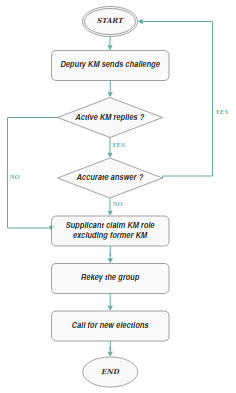
\includegraphics[scale=0.72]{figures/recovery_workflow.png}}
	\caption{Failure recovery workflow}
	\label{fig:recovery_workflow}
\end{figure}

\subsubsection{Election mutual exclusion and roles definition}

The protocol’s design assumes that a node can belong to two distinct groups in the same time. Basically, a node cannot be the KM for more than one group. Nodes dispose of a binary parameter $elected$, by default set to $False$. If a node gets elected in the context of any group it belongs to, this parameter is switched to $True$. If a node $n_i$ is affected to the two distinct groups $G_1$ and $G_2$, while also been elected KM for $G_1$, then it definitely is not and will not be the KM for $G_2$. If some election takes place in the context of $G_2$, $n_i$ will have its parameter elected already set to $True$. Hence, it just won’t broadcast its CEF score, and so won’t be promoted as a potential candidate. But this restriction doesn’t prevent the node from participating in the voting process.

In case a node other than the KM is compromised, the KM has the charge of the rekeying operation, as originally defined in MGKMP. Upon a node’s join or leave, the procedure remains the same as well. However, if it’s the KM itself which is detected as compromised or flooded with a huge charge of tasks, then a failure recovery process is instigated. When in place, the detection is done by the deputy KM.

To enhance the scheme’s performance and strengthen its decentralised side, we introduce two operational optimisations regarding tasks mainly handled by the KM. One concerns the key share during rekeying process, while the other is more about its very own generation. During a rekeying operation, the KM is responsible for new keys generation as mentioned. These new keys shall be communicated to the concerned group members. For this, the KM doesn’t necessarily have to deliver it to every node one by one. Some fellow members might already have pre-established communication channels between them, encrypted with keys known to only both of them. To save its energy and bandwidth, the KM might rely on other fellows, having low energy-consuming tasks, to relay the information in a peers-seeders fashion. Besides, upon a new node’s join, the KM doesn’t necessarily have to generate new keys for the rekeying operation. It could actually make use of prefix encryption and generate derived keys from the old ones. Nodes detaining the old keys, those are group fellows, are able to guess the new ones. But the joining node, receiving the new keys, won’t be able to climb up to the old ones, which satisfies the forward secrecy requirement. This however is applicable only to node join operation. By definition, this prefix encryption enhancement cannot work out for node leave or eviction operations.

\subsubsection{Inter-group communications management}

In the reviewed literature (Section~\ref{subsec:ch}), election-based schemes assume a CH for each group. Since proposed solutions are aimed at addressing routing problems, groups were not supposed to communicate between each other. For instance, each group has its own KM, and the latter shall mind only his groups internal business. Therefore, they manage only intra-group communication issues. However, the MGKMP leaves the door open for inter-group communications. In the original centralized scheme, the problem wasn’t even to worry about since we have one central KM for the whole network. In order to solve this issue, our solution suggest that every KM within the network is capable of operating on the inter-group level, and it’s the situation that determines which one in particular to do it. The design of MGKMP assumes that nodes hold DEKs and KEKs to secure group communications on the service level. These keys are very important, because they’re used by nodes in order to enhance the protocol’s scalability and efficiency. Nevertheless, a group by definition is a unique combination of service(s). Hence, These mentioned keys actually involve communications on the inter-group level, which we will refer as the federal level. It’s right here where the limit of previously proposed works on CH schemes bring front another limitation: if we have a KM for every group, such is our case, which entity is responsible for tasks involving more than one group ? If we look deeper these so-called federal processes, they mainly interfere during rekeying operations, the KM’s main task. So basically, the renewing of these service related keys occurs in the aftermath of a group’s membership update (node’s join, leave or eviction). Therefore, we assume that it’s the KM for the concerned which will handle the whole task. It will take of renewing the group-related keys and all the other keys requiring renewing. Then, it will communicate these keys to the concerned groups if necessary. This way, any locally elected KM can actually be the federal KM, and may assume these double role whenever the situation requires it. Handling two positions simultaneously and for a short time slot makes this solution efficient. Allowing all so-called local KMs to do it makes the inter-group key management decentralised, and thus, the solution scalable and compatible with heterogeneous networks.

\subsection{Election process}

This section describes the election process. It defines notations related to the operation, and enumerate its different steps.

\subsubsection{Group Key}

Since the election takes place in the context of a one particular group, the election procedure detailed in the forthcoming paragraph would actually require broadcast operations within this group. These transmission should be encrypted on the group level. However, the MGKMP as defined do not introduce such key, probably because it’s not actually needed for its main purpose, rekeying operations. Groups were basically designed to be logical and completely transparent to the application. As for Key Management and rekeying processes, we can do with just service keys and subgroups keys, no need for group keys. Thus, in order to secure communications with in a group without limiting ourselves to subgroup constraints, we have one existing solution. Since a group is a unique combination  of services, we could secure the message by encrypting over with all relevant service keys. All nodes belonging to the group are, by definition, holders of necessary keys to decrypt the message. Nevertheless, this solution turns out to be very expensive in terms of processing. Therefore, we introduce in this section a Group Key. We denote $K_i$ the Group Key of the $i^{th}$ group, held by all group members. This assumption increases very slightly the storage overhead for nodes. But, it saves much more in the processing overhead, and thereby less energy consuming.

\subsubsection{Notations and messages glossary}

\begin{equation}\label{eq6}
	EM1: CH \Rightarrow G_i : \langle\; \varnothing\; \rangle_{K_i}
\end{equation}
a call for election broadcasted by either current KM or its deputy

\begin{equation}\label{eq7}
	EM2: u_k \Rightarrow G_i : \langle\; c_k\; \rangle_{K_i}
\end{equation}
CEF score broadcast by potential candidate

\begin{equation}\label{eq8}
	EM3: u_k \Rightarrow G_i : \langle\; m,\; n\; \rangle_{K_i}
\end{equation}
vote broadcast by elector node, where $u_m$ and $u_n$ are the voted KM and supplicant respectively

\begin{equation}\label{eq9}
	EM4: u_m \Rightarrow G_i : \langle\; \varnothing\; \rangle_{K_i}
\end{equation}
KM role claim broadcast

\begin{equation}\label{eq9}
	EM4_{bis}: u_n \Rightarrow G_i : \langle\; \varnothing\; \rangle_{K_i}
\end{equation}
supplicant role claim broadcast

\begin{figure}[htbp]
	\centerline{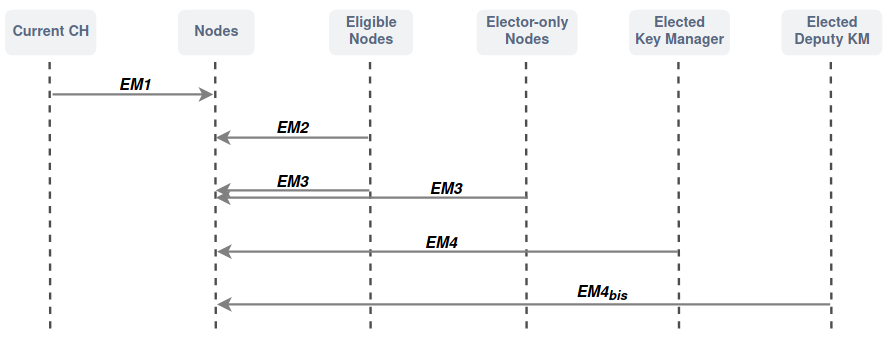
\includegraphics[scale=0.40]{figures/election_exchange.png}}
	\caption{Election process message exchange}
	\label{fig:election_msg_exchange}
\end{figure}

Fig.~\ref{fig:election_msg_exchange} demonstrates the assumed sender of each message. The timeline order of sending these messages goes from $EM1$ to $EM4$/$EM4_bis$. As shown in the figure, all message are actually broadcasted by their source nodes to the whole group.

\subsubsection{Election procedure}

The choice of the KM and eventually its deputy is based on an election procedure, during which nodes will vote for the most reliable KM. The procedure’s outcome must satisfies the election of a technically reliable and secure KM, while consuming the minimum of bandwidth.

\begin{figure}[htbp]
	\centerline{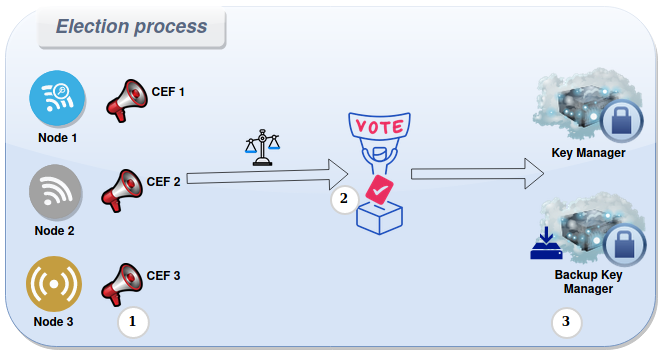
\includegraphics[scale=0.50]{figures/election.png}}
	\caption{Election procedure}
	\label{fig:election_proc}
\end{figure}

When an election trigger is pulled, the current CH, whether KM or supplicant, will instigate the election procedure. It first broadcasts the message $EM1$ to the relevant group. This message is a call group members for elections. Once group fellows receive this message, each potential candidates will update their CEF score. These nodes must definitely have their $elected$ parameter set to $False$. Nodes which $elected$ parameter is set to $True$, are deemed not to run and would skip this step. For each running node, if its updated CEF score is higher than the $rt$, it then braodcasts the message $EM2$ to group members. This message contains the updated CEF score and the identifier of its sending node, for others to benchmark to most reliable candidate. Followingly, nodes will receive different capacity scores from different candidates. Thereby, they dispose of a list of scores corresponding to group fellows, including their own if they’re candidates. Every node will benchmark scores in its list in order to choose the highest two. Then it will broadcast the message $EM3$, which contains identifiers of both chosen candidates for KM and supplicant roles respectively. Now every candidate node receiving this message will keep a count of which node received most votes. So theoretically, the count should be the same for every node, with the exact number of votes for the same couple of KM/supplicant, knowing who the ones are. However, due to the probabilistic aspect of networking and some nodes IoT-related liabilities, it doesn’t always work out perfectly as expected. That’s why we are keeping track of this count. If a candidate node sees that it has been elected for either role, it has to claim it. In case the node is elected as KM, it will broadcast the message $EM4$ to the group, which contains its identifier and useful coordinates. This message announces to the group that the sending node is the new KM. In case the node is elected as supplicant to the KM, it will broadcast the message $EM4_bis$ to the group, which contains its identifier. This message announces to the group that the sending node is the new deputy KM. Now this is concerning candidate nodes. For the rest of elector-only nodes, they actually go into a stall mode since sending message $EM3$. They don’t need to neither receive other nodes $EM3$ messages, nor keep track of the election progress. This will save them significant networking and processing overhead, and thus energy. For every single node, the reception of both claim messages marks the endpoint of the election procedure. This notification could be relayed through different node hops, just like the new key sharing. This helps reducing the networking overhead for the KM and make sure every node received the notifications.

\subsubsection{Election outcome}

The election’s purpose is to efficiently benchmark different nodes CEF scores, in order to select a KM and a deputy for the group. The election’s outcome is actually this KM/deputy tuple, which once the election procedure is through, they should be getting their new status. Now at the very beginning, the election had been called for by either the former KM or the former supplicant. This so-called election instigator could itself be re-elected to one of the two positions. In case the KM is the one calling for elections, there is no way it would be re-elected in either positions. Actually, this case matches only a KM rotation due to its drainage. The concerned node wouldn’t be participating in the election procedure in the first place, so this case is irrelevant. However, if the election’s instigator is the supplicant, it would take part in the elections as a candidate, and has pretty good chances to be re-elected.

\begin{figure}[htbp]
	\centerline{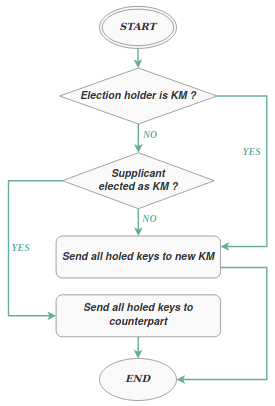
\includegraphics[scale=0.70]{figures/election_outcome.png}}
	\caption{Election outcome}
	\label{fig:election_outcome}
\end{figure}

\subsubsection{Election conflicts}

An eligible node, belonging to multiple groups, can participate in two election processes simultaneously. But if it gets elected in two distinct election process simultaneously, it shall assume the responsibilities of a KM where it’s more needed. For this purpose, a difference in the CEF score with the corresponding elected supplicant is measured. And where the difference is less significant, the node can decline the position to accept the other one. In other words, the choice goes to the group where the capability gap is wider in order to avoid under-performance issues. However, when a node is approved as a KM in a group’s election process, and as a supplicant in another, it would be accepting the KM position and declining the supplicant role. Nevertheless, if a node is simultaneously approved for supplicant in two elections, it can assume both as the supplicant role doesn’t have consequent heavy assignments.

For the following detailed example, we introduce the distance measurement:

\begin{equation}\label{eq5}
	d\left(n_1, n_2\right)  = e_k \; .\; \left( w_s s_k + w_n n_k +  w_p p_k \right)
\end{equation}

where
\begin{math}
	\left\{
	\begin{array}{l}
		c_k: capacity\; score\; of\; a\; node\; u_k\\
		w_s: storage\; capacity\; weight\\
		w_n: networking\; capacity\; weight
	\end{array}
	\right.
\end{math}\\

Let $n_i$ a technically capable node belonging to the groups $G_1$ and $G_2$, with both groups having an ongoing election process each. Let ${n_i}^1$ and ${n_i}^2$ also technically capable nodes belonging to $G_1$ and $G_2$ respectively. If parameter elected for $n_i$ is off, then it can broadcast its CEF score within the context of both groups as a potential candidate. If it receives an approval for the KM in a $G_1$ related election with ${n_i}^1$ as supplicant, it also receives approval as KM in the $G_2$ related election process with ${n_i}^2$ as supplicant, an arbitration should take place. Since the election is based on the CEF score, $n_i$ will measure the differences $d_1$ and $d_2$ with the node ${n_i}^1$ and ${n_i}^2$ respectively. $n_i$ will assume the charge of KM for the group related to the corresponding node with $m = max\left(d_1,\; d_2\right)$. Hence, it will decline the election approval for the other group, letting its corresponding deputy take over.

Fig.~\ref{fig:election_conflicts} illustrates the participation of the blue node in two separate elections with in the context of two different groups. The figure demonstrates how to proceed in case the blue node was elected as either KM or supplicant in both elections simultaneously. Table~\ref{tab:election_conflicts} sums the three cases up.

\begin{figure}
	\centering
	\begin{subfigure}[htbp]{0.3\textwidth}
		\centering
		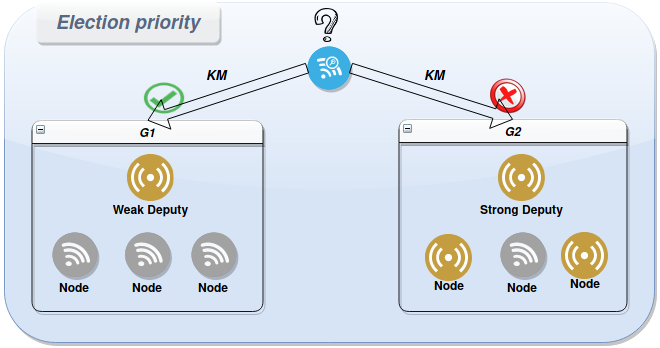
\includegraphics[scale=0.20]{figures/election2.png}
		\caption{Case 1}
		\label{fig:case1}
	\end{subfigure}
	\vfill
	\begin{subfigure}[htbp]{0.3\textwidth}
		\centering
		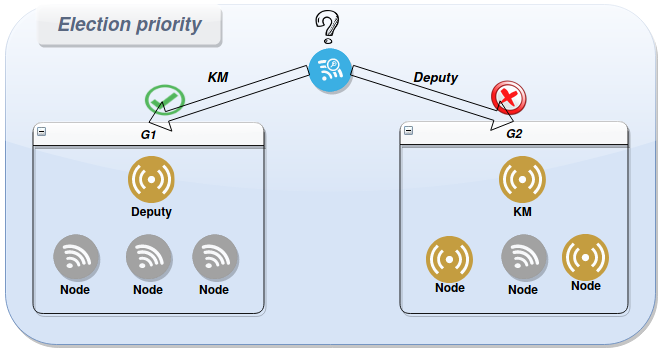
\includegraphics[scale=0.20]{figures/election3.png}
		\caption{Case 2}
		\label{fig:case2}
	\end{subfigure}
	\vfill
	\begin{subfigure}[htbp]{0.3\textwidth}
		\centering
		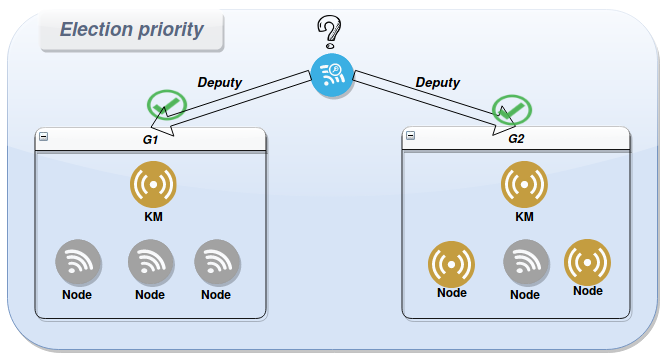
\includegraphics[scale=0.20]{figures/election4.png}
		\caption{Case 3}
		\label{fig:case3}
	\end{subfigure}
	\caption{Election conflicts}
	\label{fig:election_conflicts}
\end{figure}

\begin{table}[htbp]
	\caption{Election conflicts}
	\begin{center}
		\begin{tabular}{|c|c|c|c|}
			\hline
			\multicolumn{2}{|c|}{}&\multicolumn{2}{|c|}{\textbf{$G_1$ related election}} \\
			\cline{3-4} 
			\multicolumn{2}{|c|}{}& \textbf{\textit{Key Manager}}& \textbf{\textit{Supplicant}} \\
			\hline
			\textbf{$G_2$ related election}& \textbf{Key Manager}& verboten & verboten\\
			\cline{2-4}%\hline
			\textbf{$G_2$ related election}& \textbf{Supplicant} & verboten & allowed\\
			\hline
		\end{tabular}
		\label{tab:election_conflicts}
	\end{center}
\end{table}

\subsection{Failure recovery process}

There are three situations which could be qualified as failures requiring the instigation of a recovering process. In the first one, the KM is somehow unavailable, due to some flooding or a technical breakdown. The second situation concerns an attack leading to the compromise of the KM. And the last one is when a node is overworked and willing to hand over its responsibilities.

\begin{figure}[htbp]
	\centerline{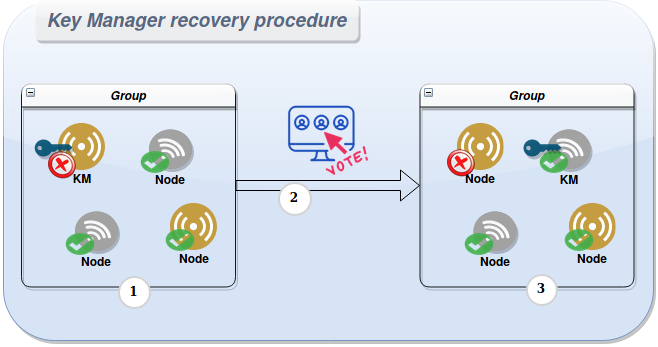
\includegraphics[scale=0.50]{figures/recovery.png}}
	\caption{Key Manager recovery routine}
	\label{fig:km_recovery}
\end{figure}

Starting with the first situation, the KM might be subject to overworking due to the important networking and processing overhead it has to bare. This could also be caused by veiled activities. Unless it has specific procedures to curb this burden, it obviously makes it vulnerable against breakdown. When the unwanted occurs, it’s first detected by the deputy KM, thanks to the regular check over procedure. Since the active KM will be unable to answer its deputy’s requests, this will let the latter know it’s technically down. From here, the supplicant broadcasts a claimer message to the group announcing that it’s taking over the leadership of the group. The former KM is excluded from the broadcast though. Then it starts a rekeying operation of the group. An finally, it calls for a new election to redefine who is the KM and his deputy on solid basis. We actually have no idea whether the breakdown is due to technical dysfunction or malicious attack such as DDoS. It could even be compromised by a malware, which prevents the reply upon check over to make it look like a normal breakdown. Keeping the former KM in the loop is exactly taking the risk of having a potential Trojan horse inside its network, without bothering taking any precautions. This significantly increases the resilience of the protocol.

\begin{figure}[htbp]
	\centerline{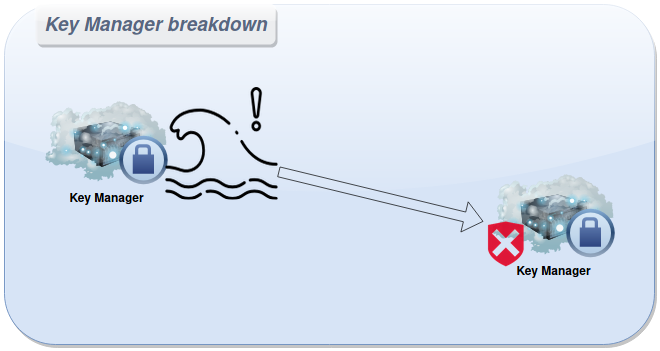
\includegraphics[scale=0.50]{figures/flooding.png}}
	\caption{Key Manager breakdown}
	\label{fig:km_breakdown}
\end{figure}

For the second situation, either we assume that we have a security entity (SE) physically separate from the KM (an IDS for example). It’s this component that guarantees the detection of eventual cyber attacks, and therefore, the instigation of the recovery process. Or, when in place, we can use the supplicant as a controller to detect the compromise, and so launch the recovery process. In the first case, we don’t consider the detection phase since it’s totally handled by the SE. But once the dysfunction is detected, the SE report directly to the KM deputy. In the second case, it’s the deputy KM that detects the compromise of its leader. The scenario would start with the supplicant receiving an inaccurate reply from the KM, upon a regular check over request. The inaccurate reply is basically a wrong answer to the deputy’s challenge. In both cases, the latter broadcasts then a disclaimer message to the concerned group fellows announcing that he is the new KM, while excluding the former one from the broadcast. It starts a rekeying operation after that of the group, since here we know for sure we have a node (the former KM) to evict. And finally, it calls for elections to settle a new appropriate KM, or at least fill in the vacant position of the supplicant.

\begin{figure}[htbp]
	\centerline{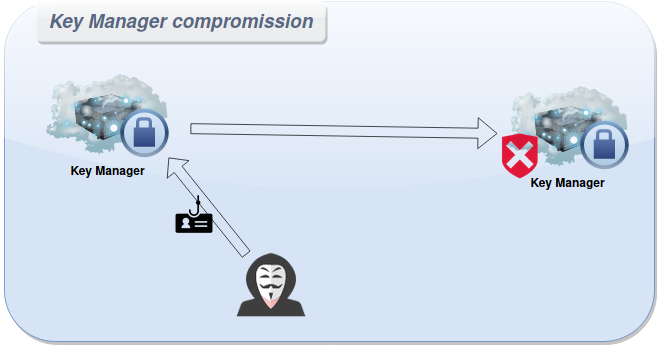
\includegraphics[scale=0.50]{figures/compromission.png}}
	\caption{Key Manager compromise}
	\label{fig:km_compromission}
\end{figure}

In this last situation, the KM isn’t necessarily suffering from any particular malfunctioning. For several reasons, it may choose to hand over its responsibilities to another node. It actually foresees some situation where, for application reasons, the KM will have additional expensive tasks to handle besides the Key Management ones, exceeding its capacities. The step off cause might simply be the KM leaving the group too as part of the application. Instead of forwarding the task to the deputy, it first calls for anticipated election in which it would not be a candidate. The election will output a newly KM . Only then, the desisting KM hand over the role to the latter.
%
%[TODO dig and develop the 3rd case]

\begin{figure}[htbp]
	\centerline{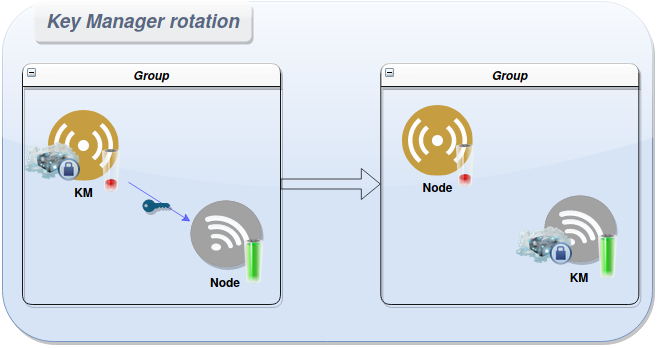
\includegraphics[scale=0.50]{figures/rotation.png}}
	\caption{Key Manager turnover}
	\label{fig:km_turnover}
\end{figure}

The scheme, as explained, introduces a supplicant which monitors the active KM and ready to take over in need, while actually allowing any node to be the KM itself. This alongside the performance optimisation introduced for new key sharing, are made up to address the issue of \textit{\textbf{single point of charge}}. With in the same progress line, the capability-based election process concatenated with the failure recovering processes, their conditions and the supplicant’s monitoring are actually made up to address the issue of \textit{\textbf{single point of trust}}. This way, the overall election-based scheme solves the issue of \textit{\textbf{single point of failure}}, by locking on the different reasons which led to this problem in the first place, as well as its unexpected consequences.

\begin{figure}[htbp]
	\centerline{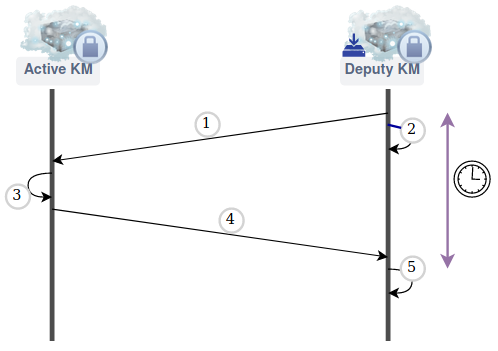
\includegraphics[scale=0.50]{figures/check_over.png}}
	\caption{Check over message exchange}
	\label{fig:double_check_exchange}
\end{figure}

Fig.~\ref{fig:double_check_exchange} illustrates the message exchange for a routine check over procedure. Above labeled steps correspond to:

\quad(1) Challenge request

\quad(2) Set timer on

\quad(3) Answer computation

\quad(4) Challenge reply

\quad(5) Set timer off + Challenge validation

The challenge validation implies both, a correct answer to the request and a response time within the set timeout.

An alternative routine would be the supplicant listening to the active KM, whereas the latter sends regular messages to its deputy announcing it’s still up. For integrity consolidation these messages have to be cryptographically signed. This pulse-check routine reduces the networking overhead by a factor of two. Although from a security point of view, it’s much less reliable than the check-over routine previously described.

In order to combine advantages of both routines, we define a hybrid solution, where regular checks are performed every time lapse, referred as $\Delta$t. These checks are mostly simple pulse-checks. But every certain number of time slots $\Delta$t, referred as $nc$, we perform the double check-over routine.

\begin{figure}[htbp]
	\centerline{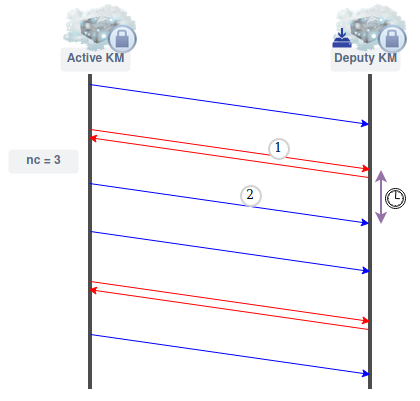
\includegraphics[scale=0.50]{figures/check_routine.png}}
	\caption{Check Over routine}
	\label{fig:check_over_routine}
\end{figure}

This way, we ensure availability and integrity of the KM, while significantly reducing the networking and processing overhead for both parties. $\Delta$t and nc are settable and configurable parameters, since depending on the actual use case, the balance between performance and security might flip to either side. If we want to keep only the first routine, one can just set $nc$ to $nc = null$. The bigger $\Delta$t is, the smaller the networking overhead is. Fig.~\ref{fig:check_over_routine} illustrates this hybrid solution, with:

\quad(1) Double-way check-over routine

\quad(2) One-way check-over routine

\subsection{Security analysis}

The CEF score is intentionally designed to be an average value totally blending regarding the input values. It’s actually more secure if the CEF score doesn’t leak any data about a node’s real capabilities in terms of networking, storage and processing. Knowledge of some physical properties of a device can be used to mount cryptanalytical side-channel attacks. During an election process, any group member node $u$ shall be able to capture CEF scores of other fellow nodes. But it won’t need these information as long as it’s a fellow member of the group and holds required keys to decipher transiting communications. When $u$ leaves the group or gets evicted, the MGKM protocol relies on the group rekeying in order to guarantee forward secrecy. The recently leaving (or evicted) node $u$ can seek to decipher group’s communications based on its previously acquired knowledge on communicating entities. This way, forward secrecy is put at risk. This also applies for a recently joining node $v$. During the first election process after its join, different nodes will be broadcasting their respective CEF scores, which express their respective physical capacities. The node $v$ might then use these acquired scores to carry out side-channel cryptanalysis attacks on encrypted messages collected before its join. This way, backward secrecy is put at risk. Since the CEF’s output is a single dark value, it will therefore prevent these category of cryptanalysis attacks. Hence, our solution maintains forward and backward secrecy properties.

When a node $u$ acting as KM is compromised and evicted, the supplicant immediately takes over the group leadership and rekeys the group, while excluding the former KM from this rekeying process. Only afterwards it calls for an election and kicks the election process off. Messages related to the election which would take place will be encrypted using a newly generated group key. By applying the forward secrecy principle guaranteed by the rekeying process, the former compromised KM will hence be unable to decipher them. The group’s communications are then secure.

Another security issue had to be considered when designing the check over process. As previously hinted, the simple check over routine utilizes cryptographic message signature only as a security measure to authenticate the KM. However, the double check over routine utilizes challenge-response authentication which can be (but not necessarily) coupled with cryptographic message signature as security measures. The latter is obviously more secure, but less efficient. The combination of how all of this will be implemented is left to the eventual R\&D engineer who might take over the protocol. What actually interests us here is the foreseen security cradle put in place for the overall check over process. Now both considered measures have their own advantages and drawbacks, with the challenge-response authentication slightly safer. Nevertheless, none of both can be taken for granted. On one hand, new attacks on both keep surfacing constantly. On the other hand, both are hardened and enhanced continuously. Besides, these measures themselves bring their own parameters and vulnerabilities. As seen in Section~\ref{subsec:cryptography}, the choice of message authentication codes and signature algorithms can have a huge security impact. In the same line, different challenge-response protocols for different situations exist. The engineer implementing the process knows his own use case and security risks. Therefore, he knows better which combination of all this fits best.

In short, the check over process intentionally embeds two different and combinable security measures. The objective is to offer a maximum of options for different security situations.

\subsection{Discussion}

The following discussion brings nothing new in term if technical specification. But since this a fundamental research work, it's more destined, but not only, to any eventual engineer who might be implementing the solution. This paragraph actually tries to give a glimpse on how practical the solution is and what kind of asset and disadvantage the above technical description can have on the implemented system.

\subsubsection{Flexibility and adaptability}

The main drawback of this scheme, is the networking overhead that comes with. Despite the suggested optimisations, we still have a high number of required messages to undergo related procedures and processes. In order to get over this lack, the scheme should be designed in a flexible way.

For the protocol’s operational mode, the CH rotation has to be implemented carefully, and sometimes, even set as optional. This could be very well relevant to some applications where the KM’s choice is static and permanent (eg. Cloud server). In this case, all message exchange relevant to CH rotation is probably useless and a waste of bandwidth and energy.

Besides, the supplicant role should be optional. We can’t be always sure whether we will dispose of enough qualified candidates for both roles. And sometimes, the infrastructure could designed in a way that one particular component is intended to be the KM for his group. In which case, the engineers building the infrastructure could have foreseen alternative measures to sort out any failure in the KM. Furthermore, the supplicant plays also a security role as it monitors the KM’s availability. Depending on the global infrastructure and the KM’s ecosystem, this role could be obsolete since there is some other component doing it. In the same line of thought, this so-called powerful KM could foreseen by its implementing engineers to cover more than one group. Thereby, the mutual exclusion in elections should be optional as well, in particular, disabled. In this direction, it seems at first we’re heading back towards the original centralised KM scheme. Nevertheless, the idea of the election-based scheme is to tackle the issue of single point of failure. But the last call is left to the engineer implementing the protocol, so that it offers the protection it claim when necessary. Besides, the scheme introduces itself as a compromise between centralised (unique KM) and fully decentralised (Blockchain) schemes. This way, among n groups, we can have one or some of them managed by one capable KM, technically just by disabling an option, while the rest of the groups dispose of their own elected KM. So here the scheme doesn’t cover the whole infrastructure, but it’s used right where it’s needed to tackle the central problem previously defined. And this is particularly useful for heterogeneous networks. This also facilitates migration from centralised solution to this one.

As for the election process, the elected parameter blocking mode has to be implemented in a way it can only be enabled manually. The feature should basically be optional. This feature is useful in some cases where we might have some very battery-weak devices. Despite the set eligibility threshold, just the computation of the CEF and the preliminaries could be, for some devices, enough for the battery to be rolled out. Nevertheless, this option isn’t pertinent for all IoT use cases. And since it brings in restrictive measures for concerned nodes, then it should definitely be configurable only manually depending on the application.

The eligibility definitely cannot be stiff. In order to improve the scalability and adaptability of the protocol regarding heterogeneity, CEF threshold has to be optional and configurable as well. Depending on the application, we can have very different scales of devices power. Thereby, the very definition of a powerful node would change. Hence, we shall be able able to lower down our standards, even sinking it til 0 if necessary. On the other side, we could be willing to top it up, if the engineer implementing is sure about the robustness of his devices and his need for a very reliable KM. This CEF feature might also be left open for more input criteria (or less) depending on the use case. Nevertheless, it has always to remain as static as possible and least possible dependant on dynamic inputs. The latter actually can increase the turn over rate for the score’s update, and so, an increase in the computation overhead.

Concerning the overall architecture of the protocol, it actually relies on one KM assigned to one group basically. This should be extensible for other layers of the infrastructure, such as having one KM per service or per subgroup. Such architectures and configurations have to be thought over and studied in depth, in order to conclude on their utility, efficiency and feasibility.

\subsubsection{Inter-group communications management}

Another approach would be based on a double layer election. The first defined KM election would be regarded as a local group election. We introduce a federal election which takes place between different local KMs, in order to elect a federal KM. The latter would then assume a double role, (i) managing his own group’s keys and (ii) handling inter-group related keys. The local KMs are the only eligible candidates, and in the same time, the only voters. The rest of the election process goes the same as for the local one. This approach has the advantage that it bypasses all possible management conflict which might pop up according to the first suggestion. Typically, this might occur when the rekeying process concerns a node belonging to different groups sharing the same service. Hereby, more than one KM is supposed to handle the service keys, making a part of the process redundant between different concerned KMs. A drawback however shines when it comes to profitability. This approach is less scalable and efficient than the previous one.

\section{Simulations and results}
\label{sec:simulations_results}

A simulator of the MGKMP was developed as part of the PhD thesis \cite{kandi_lightweight_nodate} anterior to this work. After studying the code source, the program was actually implemented to simulate the protocol's rekeying process and sub-grouping algorithms. Thus it's not fit for this use case. Working on this simulator to adapt it was considered indeed. However, this would have taken much more time than implementing a new one dedicated to the ongoing situation. The second solution was picked, because the simulation phase came at a time when the conference deadline for paper submission was closing in.

\subsection{Simulator implementation}

Two simulators were implemented with different levels of success. The programming language of choice for both is \emph{Python3}. The first is much more complete and realistic, but has a lot of bugs. The second one is simpler, but still produced some decent results. The development approach adopted is object-oriented.

First of all, I thought of implementing a simulator, which will simulate the whole MGKMP architecture. In other terms, the simulator actually implements possible entities such as nodes, KM, groups and subgroups. The communication between different nodes takes place via network sockets. The simulator uses the \emph{select} function from the \emph{Socket API} to handle connections for every node. The simulated algorithms mainly include those related to the election-based scheme, ie. the election and  check-over processes. The messages exchanged were also implemented to be encrypted, to provide the most realistic environment possible. This simulator is pretty sophisticated, so its implementation requires several functions management and consequent debugging. Due to time constraints, it couldn't be finished. So I switched to a similar simulator, but with some features cut off.

The second simulator doesn't emulate the MGKMP architecture entirely. It only considers one group with several nodes, two of which are KM and Supplicant respectively. It does implement a messaging structure. But communications and encryption are actually abstracted, they go through the \emph{Simulator} object. The latter acts as the orchestrator running the show. It coordinates exchanges between different nodes and calls election related algorithms when needed. So this simulator is only good enough to emulate the algorithmic behavior of the developed solution, as well as the influence of different parameters variation.

The \emph{Node} object has two different categories of attributes. First, it has physical capabilities such as radio range and processing capacity. Those values are random, attributed at the simulation's start and remain unchanged all along. They are different for every node. Second, it also has volatile attributes which tend to evolve overtime, such as the percentage of processor in use and residual energy. These attributes start with the same values for all nodes. For example, the starting residual energy for all nodes is set to $re = 1000$, which is the maximum. Then it decreases overtime according to the simulation's events at a different pace for each node. Capabilities values aren't realistic, but rather based on a scale in such a way to have credible comparisons.

In order to generate results, the main program is implemented in \emph{results.py}. It starts a simulation according to given parameters ($\Delta t$, $nc$, $rt$ \ldots). Then, it stimulates different processes such as election or check-over routines. On every new event, it takes snaps, which mean it gathers information about all nodes and simulation status and stores them in a file. Based on these files, the program can generate graphics using the \emph{matplotlib} library.

\subsection{Simulation results}

In the following examples, we assume that a node which was previously elected KM cannot be re-elected. Thus to measure the influence of KM turnover on the overall organization.

The simulator initiates 8 nodes at first, none of which is KM nor Supplicant. These nodes are attributed random physical capacities as mentioned, so they can compute their initial CEF score respectively. The initial status is saved to \emph{snap00}.

In the first scenario (see Appendix~\ref{app:example1}), the simulator instigates a first election, during which \emph{Node 6} is elected KM and \emph{Node 7} is elected Supplicant. Then it instigates a second election, during which \emph{Node 7} is elected KM and \emph{Node 1} is elected Supplicant. Fig.~\ref{fig:sim_exmp1} illustrates the energy and CEF score evolution of \emph{Node 7}. Between $t = 0$ and $t = 3$, the node acted as Supplicant and its energy is hence decreasing. The second election took place between $t = 3$ and $t = 6$, after which \emph{Node 7} became KM. What the figure illustrates, is that during the same time lapse ($\Delta t= 3$), the election process if far more exhausting than the check-over.

\begin{figure}[htbp]
	\centerline{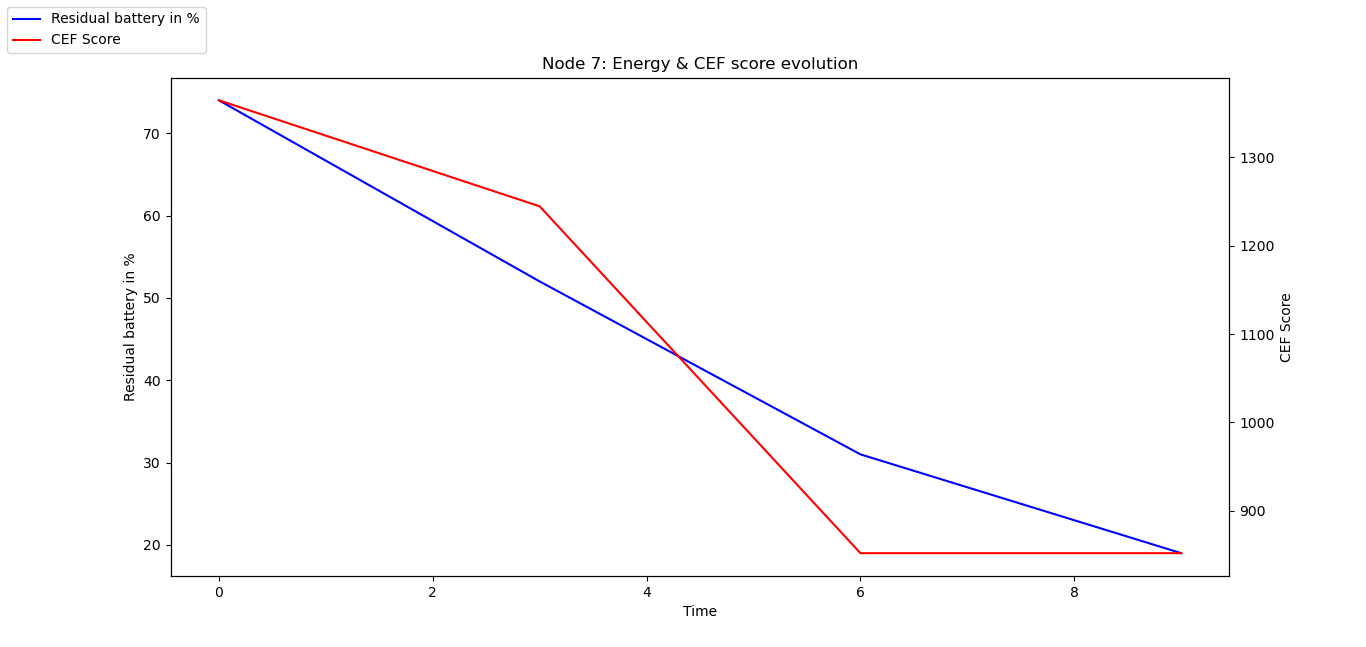
\includegraphics[scale=0.35]{figures/simulation/energy_cef_evolution.png}}
	\caption{Node 7: Energy \& CEF score evolution}
	\label{fig:sim_exmp1}
\end{figure}

In as a second scenario, the simulation tries to assess the influence of $nc$ value on the solution. The election process is a random event. Hence, I concentrated more on the check over process, since I have more control on its occurrence frequency.

Let's assume that a check process, whether simple or double, is an atomic operation. We fix the time gap between two consecutive checks to $\Delta t = 2$, and the simulation duration is fixed on 36 time units. The simulation consists in running the check-over routine over the simulation duration straight with different values of $nc$, and measure the energy consumption for both, the KM and its deputy. The $nc$ value range goes from 1 to 30. Intuitively, a decrease in consumed energy during the simulation is expected as $nc$ is increased, since a one-way check consumes less than a double one. From an energy perspective, we tend to increase this value. From a security perspective, we tend to decrease it. The objective is to find a satisfactory compromise.

\begin{figure}[htbp]
	\centerline{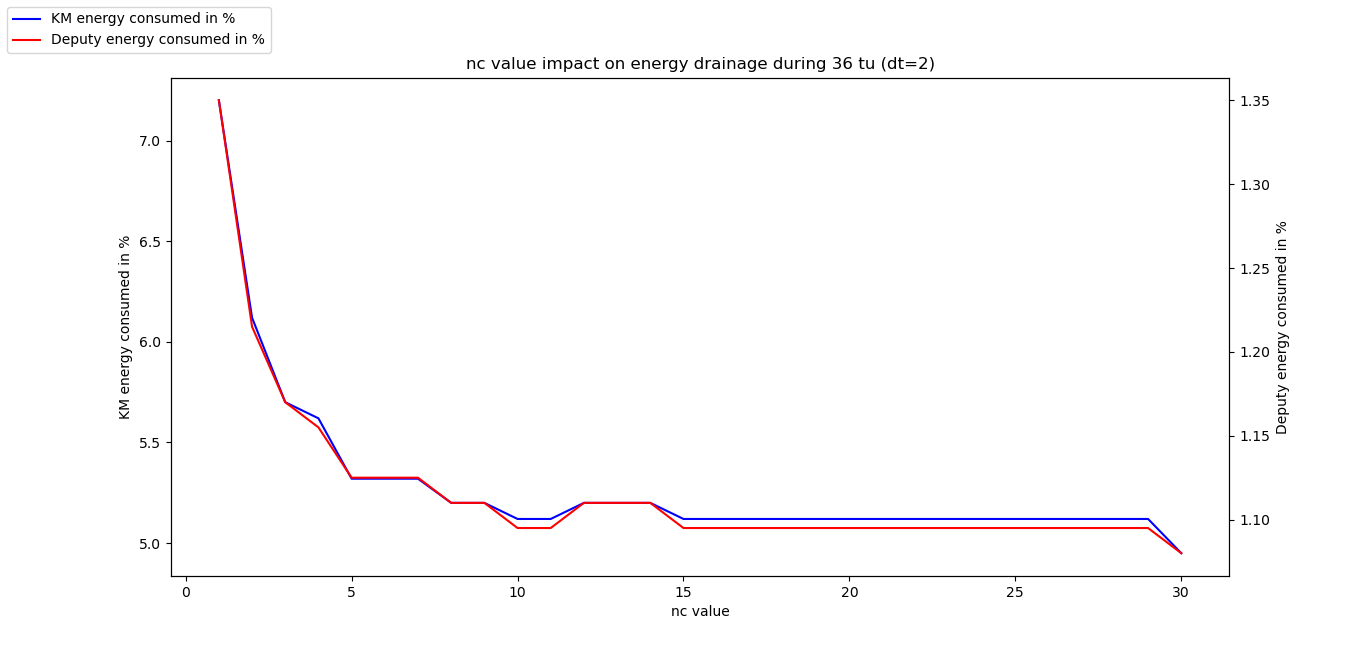
\includegraphics[scale=0.35]{figures/simulation/nc_energy.png}}
	\caption{Variation of energy drainage according to $nc$ value}
	\label{fig:sim_nc_impact}
\end{figure}

Fig.~\ref{fig:sim_nc_impact} shows that this compromise can be quickly found, and it’s valid for our two measured entities. The gain in energy grows pretty fast as we increase $nc$ value between $nc=5$ and $nc=10$. Therefore, our algorithm is able to reach good energy performances, while keeping a certain security level ensuring the KM’s integrity. There is a slight illogical increase in energy between $\Delta t = 12$ and $\Delta t = 14$ though. The reason isn't clear, but it could be explained by the simulator's random behavior.

It's \textbf{\textit{very important}} to note that interpretations rely only on figures shape, regardless of the scales or values. As said before, the program simulates the algorithmic behavior of protocol. So we know that in a more realistic experiment, we would still get the same figure's shape, but the output values can be different. For example, Fig.~\ref{fig:sim_nc_impact} shows that between $nc=1$ and $nc=5$, energy drainage dropped by approximately 1.9\%. It's this kind of value which is irrelevant, because physical capabilities are randomly attributed and disconnected with the physical realm.

\section{Future work}

If I pick up where I last left off, it is clear that simulations and experiments need to be pushed way further. First, simulations remain in their early stages. More tests should be carried out using a more sophisticated and realistic simulator. Second, real laboratory experimentation has to be carried out to observe the divergence between simulations and experiments, and eventually address the gap. The simulator itself isn't fully implemented. From a functional point of view, many features are poorly developed. For instance, a node can have a negative battery value, absolutely mind blowing. That's because until this point, these features aren't required to retrieve the needed measures. But as the simulations get more advanced, it's better to have something more complete. From a structural point of view, it's also better to make the simulations more realistic, regarding how nodes are organized and communicating. This actually goes back to finishing the second simulator which didn't work out in this internship.

Another task to look closer concerns the algorithms complexity. In this chapter, no such mathematical study was made, and yet it's important to assess. It was shown through simulations that election and check-over algorithms don't have the same energy consumption for example. A more more profound algorithmic study can reveal the exact difference, and eventually contribute in the complexity optimization.

Moreover, all issues described in Chapter~\ref{chap:mgkmp} need to be treated the same way as the Key Manager. In particular, the work on the CEF score done in this internship can be inter-crossed with the subrouping sequences (Section~\ref{subsec:subgroups}) and $mc$ values.
\chapter{IoT Security engineering}
\label{chap:iot_security}

This Chapter treats IoT security from an industrial engineering perspective. At this point of the internship, it was decided to cut the research work off, and turn more towards practical subjects. This marks the end of \emph{Stage 1} and the start of \emph{Stage 2}.

\section{Threats landscape in the IoT}

\subsection{Main threats}

As for all information systems, one of the most common threats IoT devices are facing is malware. In difference with usual malware we deal with on computer systems, IoT malwares are very often cross-architecture, because IoT devices themselves are based on different physical and processor architectures. That’s to say that antagonists are adapting their malicious payloads to the heterogeneity in IoT. Besides the damage a malware can inflict on the system by definition, the cross-architecture side of IoT malwares make them very difficult to detect and classify. Moreover, energy-constrained devices are not likely to support complex malicious code detection systems. Alhanahnah et al. [8] made a step towards proposing a signature generation for cross-architecture IoT malwares. However, the IoT malware detection problem remains very much unsolved yet.

With over 40 billions connected objects reached by 2025, IoT devices are a very seductive tool for botnets and DDoS attacks. Going back to what has just been evoked, since some IoT devices can be easily infected with malwares in a stealthy fashion, a hacker or a hackers group can then seek to infect a large numbers of objects in order to build a botnet. IoT botnets can be used to compromise heavily secured computer systems using their powerful brute-force potential. They can also be used to conduct some of the most massive DDoS attacks, such as the Dyn attack on major DNS providers carried out by the Mirai botnet in 2016 [3]. The Dyn attack was the largest DDoS attack ever seen at its time with an unprecedented flood of 1 Tbps targeting OVH servers. Its record has only been broken by the attack on AWS servers in June 2020, with a record charge of 2.3 Tbps [11]. Once again, the attack was carried out by an IoT botnet. The exponential growth of IoT connected objects is only democratising these kind of lethal attacks, and posing more serious security challenges in IoT networks security. Molesky and Cameron [9] proposed a solution based on the “White Worm” technology, which uses the very technical basis of this threat and turn it up into an asset used for benign purposes. The scheme remains pretty theoretical though, and a lot is yet to be done to bring the concept into a realistic application.

Another major threat in IoT is data privacy, and this concerns some of the most common IoT applications. For example, IoT connected objects are more and more used in healthcare and smart homes. In those kind of applications, we usually have wireless sensors and other types of objects gathering and processing intimate (eg. smart homes) and sensitive (eg. healthcare) data about individual’s. Therefore, IoT communications are a top priority target for network attacks, generally conducted by actors seeking to compromise either the confidentiality or the integrity of the transmitted data.

\subsection{IoT Malwares}

\subsubsection{BashLite}

IoT DDoS malware which comes with a C\&C \cite{securityintelligence}. Most BASHLIFE attacks are simple UDP, TCP floods and HTTP attacks. BASHLIFE infect a IoT device by brute-forcing its telnet access using known default credentials. One interesting aspect of BASHLIFE is that malware payload deployed in IoT devices has the BASHLIFE's C2s IP addresses hard-coded into it and are easier to monitor. Most of the infected devices are located in Taiwan, Brazil and Columbia. The source code of BASHLIFE was partly leaked in early 2015 and has led to many variants. BASHLIFE is considered the predecessor of Mirai and is in direct competition for vulnerable IoT real estate.

BASHLIFE/Lizkebab/Torlus/gafgyt is one of the popular malware which infects Linux based IoT devices to launch DDoS attacks. It was reported that BASHLIFE is responsible for enslaving over 1 million IoT devices, constituting mostly of Internet enabled cameras and DVRs. It is capable of launching attack of up to 400 Gpbs. Most BASHLIFE attacks are simple UDP, TCP floods and HTTP attacks. BASHLIFE infect a IoT device by brute-forcing its telnet access using known default credentials. One interesting aspect of BASHLIFE is that malware payload deployed in IoT devices has the BASHLIFE's C2s IP addresses hard-coded into it and are easier to monitor. Most of the infected devices are located in Taiwan, Brazil and Columbia. The source code of BASHLIFE was partly leaked in early 2015 and has led to many variants. BASHLIFE is considered the predecessor of Mirai and is in direct competition for vulnerable IoT real estate.

\subsubsection{BusyBotNet}

This IoT malware comes with embedded tools usually found on full systems dedicated for ethical hacking. These toolset include Hydra, masscan, tshark and reverse shell backdoors.

\subsubsection{Lightaidra}

LightAidra/Aidra is a IRC-based mass scanning and exploitation tool support on several architectures, namely MIPS, MIPSSEL, ARM, PPC, x86/86-64 and SuperH. Malware is designed to search open telnet ports that could be accessed using known default credentials. The source code of LightAidra is freely available on the Internet as open source project. It allows scanning and exploiting routers for make BOTNET (in rx-bot style). In addition to this, with Aidra you can perform some attacks with tcp flood.

\subsubsection{Linux.Wifatch}

Another IoT malware which infects devices and enslave them in a C\&C fashion.

\subsubsection{Lizkebab}

An IoT Botnet derived from BashLite.

\subsubsection{Mirai}

An IoT Botnet designed for DDoS attacks. It is known for being responsible for the Dyn cyberattack which occurred in October 2016. It has a C\&C malware, with an agent written in C and the controller developed in GO. Mirai is one of the most predominant DDoS IoT botnet in recent times. Mirai means "the future" in Japanese. Mirai botnet is definitely the next step in IoT DDoS malwares, however not as sophisticated as Remaiten but most effective. Mirai botnet is famous for being used in the record breaking 1.1Tbps DDoS attack with 148000 IoT devices. Mirai targets mostly CCTV cameras, DVRs, and home routers. Since the release of the Mirai source code, the number of IoT infected devices has increased from 213000 to 483000 in just two weeks. Mirai generates floods of GRE IP, GRE ETH, SYN and ACK, STOMP, DNS, UDP, or HTTP traffic against a target during a DDoS attack. More recently, Mirai has been found to be enhanced to infect Windows devices, helping hackers hijack even more devices. This enhanced Mirai could also identify and compromise database services like MySQL and Microsoft SQL running on different ports to create new admin "phpminds" with the password "phpgodwith" allowing the hackers to steal the database. The awareness of IoT botnets in recent times attributes to Mirai and the volume of traffic generated during its DDoS attacks.

\subsubsection{pnscan}

This yet another IoT Botnet was designed as a parallel network scanner.

\subsubsection{Randomware}

An IoT ransomware.

\section{Common IoT vulnerabilities \& solutions}

\subsection{Introduction}

IoT devices utilize a variety of standards and protocols for communications \cite{khan_iot_2018}, whether it’s for applications and messaging (XML, HTTP, CoAP ...), network and transport (DTLS, RPL, IPv6 ...) or physical communications (ZigBee, Bluetooth, WiFi, LoRa ...). This diversity makes it pretty challenging to design a robust generic security infrastructure, since the heterogeneous nature of IoT networks implies that we usually face hybrid networks. As a consequence, the more protocols and technologies we burden in our network, the larger the attack surface will be. Khan and Salah \cite{khan_iot_2018} carried out an in-deep study on how diverse these infrastructures can, while highlighting their strong interaction with Key Management Protocols, which is kind of the ultimate objective of this chapter.

\begin{figure}[htbp]
	\centerline{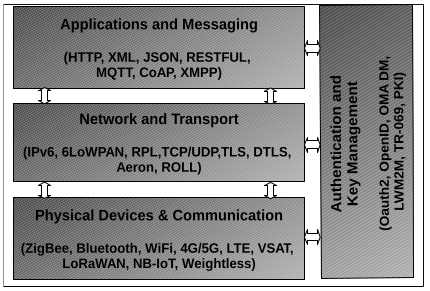
\includegraphics[scale=0.60]{figures/iot/iot_standards_protocols.png}}
	\caption{Source: \cite{khan_iot_2018} - Common IoT standards and protocols}
	\label{fig}
\end{figure}

As for every other connected device, IoT objects need to be uniquely identified on the network. For this purpose, nodes are usually identified by the mean of their MAC address and IP address. This mechanism leaves the network exposed to low-level Sybil and Spoofing attacks. This attack can be conducted by malicious Sybil nodes and may lead to serious resource scarcity, in an environment which is basically resource-constrained. Current object identification and locating mechanisms in IoT in general are exposed to a large number of vulnerabilities and operational attacks, making it a very active research topic \cite{zhang_iot_2014}.

The combination IPv6/Bluetooth is also as vulnerable as commonly used in WSNs. IEEE 802.15 standard requires fragmentation for IPv6 packets. Malicious nodes capacity to capture fragments and replay their duplicates may cause some security issues such as energy drainage or buffer overflows. This attack is known as fragmentation replay and duplication attack. IPv6 routing protocol  is also susceptible to some attacks when combined with the Routing Protocol for Low-Power and Lossy Networks, known as RPL routing attacks. It’s even more important to consider Ipv6 security, as Ipv4 won’t be able to accommodate all connected devices on the long term with their exponential number increase.

These network standards are subject to several network attacks such as session establishment and resumption attack. This consists in forging messages in order to hijack a session. In this scenario, a malicious node can spoof another legitimate node’s identity and act as a proxy between it and its counter part communicating node. In a word, weak security measures in the network will facilitate MITM-based attacks.

In addition to network related vulnerabilities, IoT objects can also present serious system issues, whether on the physical or the OS level.

%[TODO: add relevant bibliographies to previous paragraphs from [7]’s bibliography]

Appendix~\ref{app:wifi_attack} is a snippet on how vulnerable some of the commonly used network standards in Wireless Sensor Networks (WSNs) can be.

\subsection{Real-context risks \& mitigation}

A fact which stands out when looking closer at the IoT security industry, is the huge gap between the adoption of IoT for business and the adoption of IoT security practices. We require IoT security by design to ensure life-cycle sustainability for IoT devices \cite{thales2}.
When looking at different IoT solutions developed in the industry, we first look at common issues and vulnerabilities as a starting nail to track corresponding solution products. OWASP IoT Top 10 \cite{owasp-iot-10} nicely  summed up these vulnerabilities, giving an outer view of the threat landscape. In a addition to new and upcoming regulations, these issues make the conducting vectors driving the IoT security industry. No wonder they are mostly technical based, since the very purpose of developing a security technology is to hunt some specific threat.

\subsubsection{Default passwords}

A first approach to solve the problem is to look at how this password hard-coding is realized, and so, work the process straight out. The first point is that these passwords are too weak. Using a wordlist of common IoT devices passwords, an attacker is able to carry out a dictionary-based attack and take over the device. So was the case of Mirai alike attacks as explained above. The second point concerns the use of that same password all along the devices life-cycle. Users never bother to change them, assuming they are fully aware that their device can be remotely accessed using that password. Third point is that these passwords are hard-coded, so they can be quickly retrieved with old fashion reverse engineering. Moreover, they are usually stored in plain text or in a weak hash scheme, such as MD5, in order to save computing power.

The first point can fixed by requiring secure default password policies, including password length, complexity and uniqueness. Second point could be solved using password expiration and one-time password. The latter will force users to change default passwords when setting up their IoT infrastructure. Once again, we assume here that users have been notified of their device using a password in the first place. The third point is a bit more challenging to spear. As mentioned, it comes a consequence of the power-constraint nature of IoT devices. Hence, it’s difficult to work it out, without wrecking the device’s performance.

An alternative approach to address this issue is to sum up several authentication layers. Passwords is actually an authentication mechanism among others. Therefore, adding extra authentication can mitigate the risk of password compromise. This can be implemented through two-factor authentication, bio-metric authentication, Single Sign On tokens (SSO), digital certificates and PKI. 

It’s vital to bear in mind that this password issue is basically authentication related. Whereas authentication can be realized throughout who we are, what we know and what we possess. From this perspective, passwords is something we know. If it burdens vulnerabilities, we can just bypass it by exploring other information we know, alongside who we are and what we possess. An IoT devices fleet is usually relatively widespread geographically, making the  latter two authentication strategies merely feasible.

\paragraph{Solutions}

\begin{itemize}
	\item One-time passwords (OTP)
	\item Temporary one-time passwords (TOTP)
	\item Smart card based SSO
	\item eSIM
\end{itemize}

%One-time passwords (OTP)\\
%Temporary one-time passwords (TOTP)\\
%Smart card based SSO\\
%eSIM

\subsubsection{Irregular patches and updates}

Once the IoT infrastructure is set up, the device fleet remains mostly static, and that can lead to tremendous disasters. Devices come with embedded firmware. And like almost any firmware, it can be reverse engineered and pwned. Overtime, a firmware is susceptible to become obsolete and vulnerable. That’s why patches and upgrades are vital against common security vulnerabilities and 0-Days exploits.

The Satori attack is a good example to illustrate the risk \cite{arstechnica}. The attack occurred when hackers exploited critical vulnerabilities in wide range of routers (D-Link, Huawei, RealTek ...), allowing them to get a RCE, in order to build up large IoT botnets. These botnets were exploited at first to conduct massive DDoS attacks, and later on, to mine digital coins. Besides, Satori’s payload include a worm to allow the infection of neighboring devices with no human interaction needed, in a Stuxnet fashion.

The problem with upgrading IoT devices resides in the fact that these are usually widespread out there in the field. It’s difficult to deliver an update to a thermo-sensor deployed in a farm for instance. Some solutions exist though, even if they only solve the problem partially.

\paragraph{Solutions}

\begin{itemize}
	\item Pre-signed URL
\end{itemize}

%Pre-signed URL

\subsubsection{Insecure interfaces}

IoT devices aren’t standalone components. They implement network protocols for communication (e.g. Bluetooth, LPWAN ...), services for maintenance (e.g. Telnet) and applications for data processing and storage. These interfaces comes with their own vulnerabilities, whether generic or specific to the IoT implementation. Thus, they increase the attack surface.

The main strategy for mitigating this risk available right now is encryption. This particularly involves the use of digital certificates (e.g. X509). The ENISA report on “Good Practices for Security of IoT” \cite{enisa} highlights above all security by design. Security has to be bared in mind all along the device’s design and implementation, from the very cradle to the grave. The Best Practices to mitigate interface related risk involve application of ENISA good practices related to used standards. In other terms, one must apply security measures not only limited to the device itself, but take a step further to pack in the entire ecosystem and bring it under control.

\paragraph{Solutions}

\begin{itemize}
	\item Thales Trusted Key Manager
	\item Remote subscription management
	\item IQNOX IAM platform
\end{itemize}

%Thales Trusted Key Manager\\
%Remote subscription management\\
%IQNOX IAM platform

\subsubsection{Data exposure}

Smart devices are specifically designed to carry out tasks where they handle large amount of data. A common risk in IoT security is data leakage. Scandals and large-scale attacks made lack of data protection in the IoT a top concern in the industry. Whether stored data at rest or active data being exchanged, it has to be safe from unauthorized access.

All communications at all layers have to be secured, how insignificant the layer might seem. An attack on a casino reported by Darktrace in 2017 demonstrates how expensive insufficient data protection can be \cite{thesun}. The attackers in this case actually exploited lack of communications security in a smart thermometer of an aquarium exposed in a casino. They used this smart device to get a foothold in the casino’s network, then going up to the cloud, and finally exfiltrate 10Gb of the casino’s customers stored data.

The most efficient way at disposal to address this threat is cryptography. It defends against data theft for stored data and eavesdropping for over-the-network data. It preserves therefore the data privacy, integrity and confidentiality. Data at rest must, besides its encryption, be stored on an under-control host. When communicating, a secure channel with the counterpart shall be established and messages exchanged should be encrypted (confidentiality) and signed (integrity). Looking up to the previously described attack, we first notice the unencrypted communications which allowed the attackers to get their foothold in the first place. And second, the data were insecurely stored, which allowed the hackers to quickly fetch the database files and exfiltrate them.

\paragraph{Solutions}

\begin{itemize}
	\item Thales embedded Secure Element (eSE)
	\item Trusted Platform Module (TPM)
\end{itemize}

%Thales embedded Secure Element (eSE)\\
%Trusted Platform Module (TPM)

\subsubsection{IoT fleet management}

With the increase of connected IoT devices and the sophistication of its inter connection, the risk of misuse or mismanagement of some increases as well. A more and more common issue consist in IT teams not aware of what and how many connected devices they have inside their their network \cite{helpnetsecurity}. Within the same line, we are facing a rising number of “Shadow IoT and IoMT devices”. Among the most dangerous discoveries, one concerns the use of Facebook and YouTube applications of medical devices operating Windows XP. Having a medical device connected running insecure web applications on an obsolete and unsupported OS is not only a cyber threat, but a threat to human life. This kind of mismanagement made such schemes a beloved target for ransomware attacks \cite{cpomagazine}.

Therefore, it’s crucial to deploy IoT management platform whenever it’s necessary. IoT management platforms facilitates the monitoring of different devices connected to its network. It can be seen as an inventory of objects, which provides information about their status, connectivity, access logs, running apps and services ... etc. With such a global overview, one can set up security counter measures much easier, because this kind of information flow can easily fit in as an input for a SIEM or an IDS/IPS in order to automatically spot among others paranormal behavior, unusual access, collusion between subnets or VLANs, and foremost, shadow IoT devices. Obsolete or vulnerable devices can then be upgraded or patched. Improper network segmentation can be fixed. Shadow devices shall be disposed of.

\paragraph{Solutions}

\begin{itemize}
	\item Azure IoT management platform
	\item IBM IoT management platform
\end{itemize}

%Azure IoT management platform\\
%IBM IoT management platform

\subsection{Legal framework evolution}

Another vector driving the IoT security industry is the evolution of national and international regulations. Companies have to adapt their technical standards to meet requirements of laws which recently came into force. The EU voted the Cybersecurity Act in 2019, which already sets standards for IoT security manufacturers. The law was pushed by ENISA in order to curb IoT related risks. The US followed the trend with the IoT Cybersecurity Improvement Act late 2020. A bill passed on by British regulators require IoT devices sold in the UK to embed a “reasonable security feature”.
\chapter*{Conclusion}
\addcontentsline{toc}{chapter}{Conclusion}

The internship took place in two main parts, fundamental research and practical engineering. The first one was a furtherance the laboratory's research work on IoT security in general, and Group Key Management (GKM) in particular. During the second stage, I was rather wearing an engineer's hat. I was still working on IoT security though, but more from a practical view.

The first part was by far longer and much more intense compared to the second one. This part itself went through different steps. The first step of my research task was dedicated to self-learning, documentation and foremost reading academic papers. Although I have a cybersecurity background, I started the internship with almost no prior academic knowledge about security in the IoT domain. I was even much less ranged when it comes to GKM related topics. Therefore, I had a lot to catch up for at first, in order to better apprehend different scientific advances and challenges. I had to study as much as possible the concepts I was going to work on. This concerns different GKM schemes and the MGKMP at first. But then it extended to the Cluster Head (CH) architectures, when I started considering it for the developing solution. 

The second step is an in-depth study of MGKMP. The primary purpose was to identify eventual contribution axes to the ongoing research effort. The forthcoming challenges identified included possible optimizations of the protocol's theoretical design and fixing some vulnerable aspects of the protocol's features. The ultimate goal has always been making a contribution to the existing work in order to produce a research article.

The third and final step of the first stage was to focus on a specific problem. The Key Manager's issue of single point of failure was considered. A solution based on an election scheme was developed. Simulations showed some promising results. A lot of work is yet to be done though, especially for the experimental part.

By the end of the first stage, that ultimate goal mentioned had been fulfilled. A paper summing up the developed solution was published in the proceedings of the \emph{International Conference on Communications Software (SoftCOM 2021)}. This soluion was without a doubt crucial for the system. It solves the targeted problem and does what it is supposed to do. This has already been confirmed by international reviewers from the \emph{SoftCOM 2021} conference. Nevertheless, I still have doubts regarding its utility and practical implementability. The work was carried out under a fundamental research program. But at some point, it has to be transposed into a practical engineering solution. Otherwise, the whole effort would be pointless. That's why I do believe this research should never be disconnected from the field realm. Permanent links and practical evaluations should be conducted all over the way, to make sure that program doesn't loose its main objective from its sight. The program's ultimate purpose is to defend an IoT network against threats. However, how good do we know this threat and how does it operate ? Will this system really deter a malicious hacker from attacking, even a little bit ? A field study of the attackers operational mode is crucial, to avoid defending the front door while the attacker is striking pr sweeping in from behind. Foremost, its important to be confident that we are not switching to new security systems, which look safer from the outside, whereas it's rotten to the core from the inside. This said, it doesn't in any way systematically implies the system is useless. Because so much of the work achieved is brilliant and academics have confirmed it. But it's only to point some deficiency out, regarding the overall approach in the problem resolution.

I gained a lot of experience in this stage. It involved a tremendous professional research know-how. This includes how to conduct a bibliographic work, how to read academic papers and criticize them, how to manage articles using academic software (\emph{Zotero} in my case) and write my own article in \LaTeX. The research requires a lot of precision, thinking and synthesis. One always has to take into account other researchers work and their outcome. The solution development require permanent focus on the ultimate goal, in a way that despite all the sideline details, one never gets diverted or distracted. The writing of the article and its publication gave me a closer insight of the academic domain.

Second part was focused on the IoT security industry. It consists mainly in studying common IoT security risks and industrial solutions from a practical point of view. Working on real IoT systems and malware samples was at most beneficial, as I gained useful knowledge and first hand experience on IoT engineering. It raised my awareness about several types of threats, and made me look closer at different engineering solutions. I didn't go far concerning the proprietary solutions bit though, since it looked like most of them are basically snake oil commercial products.

I found the internship's overall unfolding very satisfactory on the personal level. I worked on a research task, and thus I have now a better aptitude to work in the research field. I also had some engineering tasks, and thus I gained knowledge in case I want to work in the industry. This internship actually helped me a lot in my personal development and my professional plans. Besides, the pedagogic objective of an internship is to enhance my operability after graduating. This objective couldn't have been better fulfilled.
%\chapter{Writing scientific texts in English}

This chapter was originally a separate document written by Reto
Spöhel.  It is reprinted here so that the template can serve as a
quick guide to thesis writing, and to provide some more example
material to give you a feeling for good typesetting.

% We're going to need an extra theorem-like environment for this
% chapter
\theoremstyle{plain}
\theoremsymbol{}
\newtheorem{Rule}[theorem]{Rule}

\section{Basic writing rules}

The following rules need little further explanation; they are best
understood by looking at the example in the booklet by Knuth et al.,
§2--§3.

\begin{Rule}
  Write texts, not chains of formulas.
\end{Rule}

More specifically, write full sentences that are logically
interconnected by phrases like `Therefore', `However', `On the other
hand', etc.\ where appropriate.

\begin{Rule}
  Displayed formulas should be embedded in your text and punctuated
  with it.
\end{Rule}

In other words, your writing should not be divided into `text parts'
and `formula parts'; instead the formulas should be tied together by
your prose such that there is a natural flow to your writing.

\section{Being nice to the reader}

Try to write your text in such a way that a reader enjoys reading
it. That's of course a lofty goal, but nevertheless one you should
aspire to!

\begin{Rule}
  Be nice to the reader.
\end{Rule}

Give some intuition or easy example for definitions and theorems which
might be hard to digest. Remind the reader of notations you introduced
many pages ago -- chances are he has forgotten them. Illustrate your
writing with diagrams and pictures where this helps the reader. Etc.

\begin{Rule}
  Organize your writing.
\end{Rule}

Think carefully about how you subdivide your thesis into chapters,
sections, and possibly subsections.  Give overviews at the beginning
of your thesis and of each chapter, so the reader knows what to
expect. In proofs, outline the main ideas before going into technical
details. Give the reader the opportunity to `catch up with you' by
summing up your findings periodically.

\emph{Useful phrases:} `So far we have shown that \ldots', `It remains
to show that \ldots', `Recall that we want to prove inequality (7), as
this will allow us to deduce that \ldots', `Thus we can conclude that
\ldots. Next, we would like to find out whether \ldots', etc.

\begin{Rule}
  Don't say the same thing twice without telling the reader that you
  are saying it twice.
\end{Rule}

Repetition of key ideas is important and helpful. However, if you
present the same idea, definition or observation twice (in the same or
different words) without telling the reader, he will be looking for
something new where there is nothing new.

\emph{Useful phrases:} `Recall that [we have seen in Chapter 5 that]
\ldots', `As argued before / in the proof of Lemma 3, \ldots', `As
mentioned in the introduction, \ldots', `In other words, \ldots', etc.

\begin{Rule}
  Don't make statements that you will justify later without telling
  the reader that you will justify them later.
\end{Rule}

This rule also applies when the justification is coming right in the
next sentence!  The reasoning should be clear: if you violate it, the
reader will lose valuable time trying to figure out on his own what
you were going to explain to him anyway.

\emph{Useful phrases:} `Next we argue that \ldots', `As we shall see,
\ldots', `We will see in the next section that \ldots, etc.


\section{A few important grammar rules}

\begin{Rule}
  \label{rule:no-comma-before-that}
  There is (almost) \emph{never} a comma before `that'.
\end{Rule}

It's really that simple. Examples:
\begin{quote}
  We assume that \ldots\\
  \emph{Wir nehmen an, dass \ldots}

  It follows that \ldots\\
  \emph{Daraus folgt, dass \ldots}

  `thrice' is a word that is seldom used.\\
  \emph{`thrice' ist ein Wort, das selten verwendet wird.}
\end{quote}
Exceptions to this rule are rare and usually pretty obvious. For
example, you may end up with a comma before `that' because `i.e.' is
spelled out as `that is':
\begin{quote}
  For \(p(n)=\log n/n\) we have \ldots{} However, if we choose \(p\) a
  little bit higher, that is \(p(n)=(1+\varepsilon)\log n/n\) for some
  \(\varepsilon>0\), we obtain that\ldots
\end{quote}
Or you may get a comma before `that' because there is some additional
information inserted in the middle of your sentence:
\begin{quote}
  Thus we found a number, namely \(n_0\), that satisfies equation (13).
\end{quote}
If the additional information is left out, the sentence has no comma:
\begin{quote}
  Thus we found a number that satisfies equation (13).
\end{quote}
(For `that' as a relative pronoun, see also
Rules~\ref{rule:non-defining-has-comma}
and~\ref{rule:defining-without-comma} below.)

\begin{Rule}
  There is usually no comma before `if'.
\end{Rule}

Example:
\begin{quote}
  A graph is not \(3\)-colorable if it contains a \(4\)-clique.\\
  \emph{Ein Graph ist nicht \(3\)-färbbar, wenn er eine \(4\)-Clique
    enthält.}
\end{quote}
However, if the `if' clause comes first, it is usually separated from
the main clause by a comma:
\begin{quote}
  If a graph contains a \(4\)-clique, it is not \(3\)-colorable .\\
  \emph{Wenn ein Graph eine \(4\)-Clique enthält, ist er nicht
    \(3\)-färbbar.}
\end{quote}

There are more exceptions to these rules than to
Rule~\ref{rule:no-comma-before-that}, which is why we are not
discussing them here. Just keep in mind: don't put a comma before `if'
without good reason.

\begin{Rule}
  \label{rule:non-defining-has-comma}
  Non-defining relative clauses have commas.
\end{Rule}
\begin{Rule}
  \label{rule:defining-without-comma}
  Defining relative clauses have no commas.
\end{Rule}

In English, it is very important to distinguish between two types of
relative clauses: defining and non-defining ones. This is a
distinction you absolutely need to understand to write scientific
texts, because mistakes in this area actually distort the meaning of
your text!

It's probably easier to explain first what a \emph{non-defining}
relative clause is. A non-defining relative clauses simply gives
additional information \emph{that could also be left out} (or given in
a separate sentence). For example, the sentence
\begin{quote}
  The \textsc{WeirdSort} algorithm, which was found by the famous
  mathematician John Doe, is theoretically best possible but difficult
  to implement in practice.
\end{quote}
would be fully understandable if the relative clause were left out
completely. It could also be rephrased as two separate sentences:
\begin{quote}
  The \textsc{WeirdSort} algorithm is theoretically best possible but
  difficult to implement in practice. [By the way,] \textsc{WeirdSort}
  was found by the famous mathematician John Doe.
\end{quote}
This is what a non-defining relative clause is. \emph{Non-defining
  relative clauses are always written with commas.} As a corollary we
obtain that you cannot use `that' in non-defining relative clauses
(see Rule~\ref{rule:no-comma-before-that}!). It would be wrong to
write
\begin{quote}
  \st{The \textsc{WeirdSort} algorithm, that was found by the famous
    mathematician John Doe, is theoretically best possible but
    difficult to implement in practice.}
\end{quote}
A special case that warrants its own example is when `which' is
referring to the entire preceding sentence:
\begin{quote}
  Thus inequality (7) is true, which implies that the Riemann
  hypothesis holds.
\end{quote}
As before, this is a non-defining relative sentence (it could be left
out) and therefore needs a comma.

So let's discuss \emph{defining} relative clauses next. A defining
relative clause tells the reader \emph{which specific item the main
  clause is talking about}. Leaving it out either changes the meaning
of the sentence or renders it incomprehensible altogether.  Consider
the following example:

\begin{quote}
  The \textsc{WeirdSort} algorithm is difficult to implement in
  practice. In contrast, the algorithm that we suggest is very simple.
\end{quote}

Here the relative clause `that we suggest' cannot be left out -- the
remaining sentence would make no sense since the reader would not know
which algorithm it is talking about. This is what a defining relative
clause is. \textit{Defining relative clauses are never written with
  commas.} Usually, you can use both `that' and `which' in defining
relative clauses, although in many cases `that' sounds better.

As a final example, consider the following sentence:
\begin{quote}
  For the elements in \(\mathcal{B}\) which satisfy property (A), we
  know that equation (37) holds.
\end{quote}
This sentence does not make a statement about all elements in
\(\mathcal{B}\), only about those satisfying property (A). The relative
clause is \emph{defining}. (Thus we could also use `that' in place of
`which'.)

In contrast, if we add a comma the sentence reads
\begin{quote}
  For the elements in \(\mathcal{B}\), which satisfy property (A), we
  know that equation (37) holds.
\end{quote}

Now the relative clause is \emph{non-defining} -- it just mentions in
passing that all elements in \(\mathcal{B}\) satisfy property (A). The
main clause states that equation (37) holds for \emph{all} elements in
\(\mathcal{B}\). See the difference?


\section[Things you (usually) don't say in English]%
{Things you (usually) don't say in English -- and what to say
  instead}
\label{sec:list}

Table~\ref{tab:things-you-dont-say} lists some common mistakes and
alternatives.  The entries should not be taken as gospel -- they don't
necessarily mean that a given word or formulation is wrong under all
circumstances (obviously, this depends a lot on the context). However,
in nine out of ten instances the suggested alternative is the better
word to use.

\begin{table}
  \centering
  \caption{Things you (usually) don't say}
  \label{tab:things-you-dont-say}
  \begin{tabular}{lll}
    \toprule
    \st{It holds (that) \dots} & We have \dots & \emph{Es gilt \dots}\\
    \multicolumn{3}{l}{\quad\footnotesize(`Equation (5) holds.' is fine, though.)}\\
    \st{$x$ fulfills property $\mathcal{P}$.}& \(x\) satisfies property \(\mathcal{P}\). & \emph{\(x\) erfüllt Eigenschaft \(\mathcal{P}\).} \\
    \st{in average} & on average & \emph{im Durchschnitt}\\
    \st{estimation} & estimate   & \emph{Abschätzung}\\
    \st{composed number} & composite number & \emph{zusammengesetzte Zahl}\\
    \st{with the help of} & using & \emph{mit Hilfe von}\\
    \st{surely} & clearly & \emph{sicher, bestimmt}\\
    \st{monotonously increasing} & monotonically incr. & \emph{monoton steigend}\\
    \multicolumn{3}{l}{\quad\footnotesize(Actually, in most cases `increasing' is just fine.)}\\
    \bottomrule
  \end{tabular}
\end{table}

%%% Local Variables:
%%% mode: latex
%%% TeX-master: "thesis"
%%% End:

%\chapter{Typography}


\section{Punctuation}

\begin{Rule}
  Use opening (`) and closing (') quotation marks correctly.
\end{Rule}

In \LaTeX, the closing quotation mark is typed like a normal
apostrophe, while the opening quotation mark is typed using the French
\emph{accent grave} on your keyboard (the \emph{accent grave} is the
one going down, as in \emph{frère}).

Note that any punctuation that \emph{semantically} follows quoted
speech goes inside the quotes in American English, but outside in
Britain.  Also, Americans use double quotes first.  Oppose
\begin{quote}
  ``Using `lasers,' we punch a hole in \ldots\ the Ozone Layer,''
  Dr.\ Evil said.
\end{quote}
to
\begin{quote}
  `Using ``lasers'', we punch a hole in \ldots\ the Ozone Layer',
  Dr.\ Evil said.
\end{quote}

\begin{Rule}
  Use hyphens (-), en-dashes (--) and em-dashes (---) correctly.
\end{Rule}

A hyphen is only used in words like `well-known', `$3$-colorable'
etc., or to separate words that continue in the next line (which is
known as hyphenation).  It is entered as a single ASCII hyphen
character (\texttt{-}).

To denote ranges of numbers, chapters, etc., use an en-dash (entered
as two ASCII hyphens \texttt{--}) with no spaces on either side.  For
example, using Equations (1)--(3), we see\ldots

As the equivalent of the German \emph{Gedankenstrich}, use an en-dash
with spaces on both sides -- in the title of Section \ref{sec:list},
it would be wrong to use a hyphen instead of the dash. (Some English
authors use the even longer emdash (---) instead, which is typed as
three subsequent hyphens in \LaTeX. This emdash is used without spaces
around it---like so.)


\section{Spacing}

\begin{Rule}
  \label{rule:no-manual-spacing}
  Do not add spacing manually.
\end{Rule}

You should never use the commands \lstinline-\\- (except within
tabulars and arrays), \lstinline[showspaces=true]-\ - (except to
prevent a sentence-ending space after Dr.\ and such),
\lstinline-\vspace-, \lstinline-\hspace-, etc.  The choices programmed
into \LaTeX{} and this style should cover almost all cases.  Doing it
manually quickly leads to inconsistent spacing, which looks terrible.
Note that this list of commands is by no means conclusive.

\begin{Rule}
  Judiciously insert spacing in maths where it helps.
\end{Rule}

This directly contradicts Rule~\ref{rule:no-manual-spacing}, but in
some cases \TeX{} fails to correctly decide how much spacing is
required.  For example, consider
\begin{displaymath}
  f(a,b) = f(a+b, a-b).
\end{displaymath}
In such cases, inserting a thin math space \lstinline-\,- greatly
increases readability:
\begin{displaymath}
  f(a,b) = f(a+b,\, a-b).
\end{displaymath}

Along similar lines, there are variations of some symbols with
different spacing.  For example, Lagrange's Theorem states that
\(\abs{G}=[G:H]\abs{H}\), but the proof uses a bijection \(f\colon
aH\to bH\).  (Note how the first colon is symmetrically spaced, but
the second is not.)

\begin{Rule}
  Learn when to use \lstinline[showspaces=true]-\ - and
  \lstinline-\@-.
\end{Rule}

Unless you use `french spacing', the space at the end of a sentence is
slightly larger than the normal interword space.

The rule used by \TeX{} is that any space following a period,
exclamation mark or question mark is sentence-ending, except for
periods preceded by an upper-case letter.  Inserting \lstinline-\-
before a space turns it into an interword space, and inserting
\lstinline-\@- before a period makes it sentence-ending.  This means
you should write
\begin{lstlisting}
Prof.\ Dr.\ A. Steger is a member of CADMO\@.
If you want to write a thesis with her, you
should use this template.
\end{lstlisting}
which turns into
\begin{quote}
  Prof.\ Dr.\ A. Steger is a member of CADMO\@.  If you want to write
  a thesis with her, you should use this template.
\end{quote}
The effect becomes more dramatic in lines that are stretched slightly
during justification:
\begin{quote}
  \parbox{\linewidth}{\hbox to \linewidth{%
      Prof.\ Dr.\ A. Steger is a member of CADMO\@.  If you}}
\end{quote}

\begin{Rule}
  Place a non-breaking space (\lstinline-~-) right before references.
\end{Rule}

This is actually a slight simplification of the real rule, which
should invoke common sense.  Place non-breaking spaces where a line
break would look `funny' because it occurs right in the middle of a
construction, especially between a reference type (Chapter) and its
number.


\section{Choice of `fonts'}

Professional typography distinguishes many font attributes, such as
family, size, shape, and weight.  The choice for sectional divisions
and layout elements has been made, but you will still occasionally
want to switch to something else to get the reader's attention.  The
most important rule is very simple.

\begin{Rule}
  When emphasising a short bit of text, use \lstinline-\emph-.
\end{Rule}

In particular, \emph{never} use bold text (\lstinline-\textbf-).
Italics (or Roman type if used within italics) avoids distracting the
eye with the huge blobs of ink in the middle of the text that bold
text so quickly introduces.

Occasionally you will need more notation, for example, a consistent
typeface used to identify algorithms.

\begin{Rule}
  Vary one attribute at a time.
\end{Rule}

For example, for \textsc{WeirdSort} we only changed the shape to small
caps.  Changing two attributes, say, to bold small caps would be
excessive (\LaTeX{} does not even have this particular variation).
The same holds for mathematical notation: the reader can easily
distinguish \(g_n\), \(G(x)\), \(\mathcal{G}\) and \(\mathsf{G}\).

\begin{Rule}
  Never underline or uppercase.
\end{Rule}

No exceptions to this one, unless you are writing your thesis on a
typewriter.  Manually.  Uphill both ways.  In a blizzard.


\section{Displayed equations}

\begin{Rule}
  Insert paragraph breaks \emph{after} displays only where they
  belong.  Never insert paragraph breaks \emph{before} displays.
\end{Rule}

\LaTeX{} translates sequences of more than one linebreak (i.e., what
looks like an empty line in the source code) into a paragraph break in
almost all contexts.  This also happens before and after displays,
where extra spacing is inserted to give a visual indication of the
structure.  Adding a blank line in these places may look nice in the
sources, but compare the resulting display

\begin{displaymath}
  a = b
\end{displaymath}

to the following:
\begin{displaymath}
  a = b
\end{displaymath}
The first display is surrounded by blank lines, but the second is not.
It is bad style to start a paragraph with a display (you should always
tell the reader what the display means first), so the rule follows.

\begin{Rule}
  Never use \lstinline-eqnarray-.
\end{Rule}

It is at the root of most ill-spaced multiline displays.  The
\package{amsmath} package provides better alternatives, such as the
\lstinline-align- family
\begin{align*}
  f(x) &= \sin x, \\
  g(x) &= \cos x,
\end{align*}
and \lstinline-multline- which copes with excessively long equations:
\begin{multline*}
  \def\P{\mathrm P}
  \P\bigl[X_{t_0} \in (z_0, z_0+dz_0],\ldots, X_{t_n}\in(z_n,z_n+dz_n]\bigr]
  \\= \nu(dz_0) K_{t_1}(z_0,dz_1) K_{t_2-t_1}(z_1,dz_2)\cdots
  K_{t_n-t_{n-1}}(z_{n-1},dz_n).
\end{multline*}


\section{Floats}

By default this style provides floating environments for tables and
figures.  The general structure should be as follows:
\begin{lstlisting}
\begin{figure}
  \centering
  % content goes here
  \caption{A short caption}
  \label{some-short-label}
\end{figure}
\end{lstlisting}
Note that the label must follow the caption, otherwise the label will
refer to the surrounding section instead.  Also note that figures
should be captioned at the bottom, and tables at the top.

The whole point of floats is that they, well, \emph{float} to a place
where they fit without interrupting the text body.  This is a frequent
source of confusion and changes; please leave it as is.

\begin{Rule}
  Do not restrict float movement to only `here'
  \textnormal{(\lstinline-h-)}.
\end{Rule}

If you are still tempted, you should avoid the float altogether and
just show the figure or table inline, similar to a displayed equation.

%%% Local Variables:
%%% mode: latex
%%% TeX-master: "thesis"
%%% End:

%\chapter{Example Chapter}

Dummy text.

\section{Example Section}

Dummy text.

\subsection{Example Subsection}

Dummy text.

\subsubsection{Example Subsubsection}

Dummy text.

\paragraph{Example Paragraph}

Dummy text.

\subparagraph{Example Subparagraph}

Dummy text.


%\backmatter
%\chapter*{Conclusion}
\addcontentsline{toc}{chapter}{Conclusion}

The internship took place in two main parts, fundamental research and practical engineering. The first one was a furtherance the laboratory's research work on IoT security in general, and Group Key Management (GKM) in particular. During the second stage, I was rather wearing an engineer's hat. I was still working on IoT security though, but more from a practical view.

The first part was by far longer and much more intense compared to the second one. This part itself went through different steps. The first step of my research task was dedicated to self-learning, documentation and foremost reading academic papers. Although I have a cybersecurity background, I started the internship with almost no prior academic knowledge about security in the IoT domain. I was even much less ranged when it comes to GKM related topics. Therefore, I had a lot to catch up for at first, in order to better apprehend different scientific advances and challenges. I had to study as much as possible the concepts I was going to work on. This concerns different GKM schemes and the MGKMP at first. But then it extended to the Cluster Head (CH) architectures, when I started considering it for the developing solution. 

The second step is an in-depth study of MGKMP. The primary purpose was to identify eventual contribution axes to the ongoing research effort. The forthcoming challenges identified included possible optimizations of the protocol's theoretical design and fixing some vulnerable aspects of the protocol's features. The ultimate goal has always been making a contribution to the existing work in order to produce a research article.

The third and final step of the first stage was to focus on a specific problem. The Key Manager's issue of single point of failure was considered. A solution based on an election scheme was developed. Simulations showed some promising results. A lot of work is yet to be done though, especially for the experimental part.

By the end of the first stage, that ultimate goal mentioned had been fulfilled. A paper summing up the developed solution was published in the proceedings of the \emph{International Conference on Communications Software (SoftCOM 2021)}. This soluion was without a doubt crucial for the system. It solves the targeted problem and does what it is supposed to do. This has already been confirmed by international reviewers from the \emph{SoftCOM 2021} conference. Nevertheless, I still have doubts regarding its utility and practical implementability. The work was carried out under a fundamental research program. But at some point, it has to be transposed into a practical engineering solution. Otherwise, the whole effort would be pointless. That's why I do believe this research should never be disconnected from the field realm. Permanent links and practical evaluations should be conducted all over the way, to make sure that program doesn't loose its main objective from its sight. The program's ultimate purpose is to defend an IoT network against threats. However, how good do we know this threat and how does it operate ? Will this system really deter a malicious hacker from attacking, even a little bit ? A field study of the attackers operational mode is crucial, to avoid defending the front door while the attacker is striking pr sweeping in from behind. Foremost, its important to be confident that we are not switching to new security systems, which look safer from the outside, whereas it's rotten to the core from the inside. This said, it doesn't in any way systematically implies the system is useless. Because so much of the work achieved is brilliant and academics have confirmed it. But it's only to point some deficiency out, regarding the overall approach in the problem resolution.

I gained a lot of experience in this stage. It involved a tremendous professional research know-how. This includes how to conduct a bibliographic work, how to read academic papers and criticize them, how to manage articles using academic software (\emph{Zotero} in my case) and write my own article in \LaTeX. The research requires a lot of precision, thinking and synthesis. One always has to take into account other researchers work and their outcome. The solution development require permanent focus on the ultimate goal, in a way that despite all the sideline details, one never gets diverted or distracted. The writing of the article and its publication gave me a closer insight of the academic domain.

Second part was focused on the IoT security industry. It consists mainly in studying common IoT security risks and industrial solutions from a practical point of view. Working on real IoT systems and malware samples was at most beneficial, as I gained useful knowledge and first hand experience on IoT engineering. It raised my awareness about several types of threats, and made me look closer at different engineering solutions. I didn't go far concerning the proprietary solutions bit though, since it looked like most of them are basically snake oil commercial products.

I found the internship's overall unfolding very satisfactory on the personal level. I worked on a research task, and thus I have now a better aptitude to work in the research field. I also had some engineering tasks, and thus I gained knowledge in case I want to work in the industry. This internship actually helped me a lot in my personal development and my professional plans. Besides, the pedagogic objective of an internship is to enhance my operability after graduating. This objective couldn't have been better fulfilled.

%\bibliographystyle{plain}
%\bibliography{refs}

\appendix

%\chapter{Dummy Appendix}

You can defer lengthy calculations that would otherwise only interrupt
the flow of your thesis to an appendix.

\chapter{Simulation: Scenario n°1}
\label{app:example1}

\begin{verbatim}
	[+] Starting Simulator v0.1 ...
	
	[+] Simulation init ...
	[+] Node init: ID=0
	[!] CEF score for node 0 updated to: 222.33
	[+] Node init: ID=1
	[!] CEF score for node 1 updated to: 838.24
	[+] Node init: ID=2
	[!] CEF score for node 2 updated to: 402.56
	[+] Node init: ID=3
	[!] CEF score for node 3 updated to: 621.28
	[+] Node init: ID=4
	[!] CEF score for node 4 updated to: 716.45
	[+] Node init: ID=5
	[!] CEF score for node 5 updated to: 176.04
	[+] Node init: ID=6
	[!] CEF score for node 6 updated to: 16019.43
	[+] Node init: ID=7
	[!] CEF score for node 7 updated to: 1364.79
	[+] Simulation initialized !
	
	[+] Current group status ...
	
	#### Node 1 ####
	ID:		0
	CEF Score:	222.33
	Battery:	83.5 %
	
	#### Node 2 ####
	ID:		1
	CEF Score:	838.24
	Battery:	70.3 %
	
	#### Node 3 ####
	ID:		2
	CEF Score:	402.56
	Battery:	45.3 %
	
	#### Node 4 ####
	ID:		3
	CEF Score:	621.28
	Battery:	40.7 %
	
	#### Node 5 ####
	ID:		4
	CEF Score:	716.45
	Battery:	74.4 %
	
	#### Node 6 ####
	ID:		5
	CEF Score:	176.04
	Battery:	39.1 %
	
	#### Node 7 ####
	ID:		6
	CEF Score:	16019.43
	Battery:	78.4 %
	
	#### Node 8 ####
	ID:		7
	CEF Score:	1364.79
	Battery:	74.9 %
	
	[+] Snapshot saved to snap00 !
	
	[!] CEF score for node 0 updated to: 122.6
	[!] CEF score for node 1 updated to: 734.24
	[!] CEF score for node 2 updated to: 315.78
	[!] CEF score for node 3 updated to: 528.52
	[!] CEF score for node 4 updated to: 641.64
	[!] CEF score for node 5 updated to: 153.16
	[!] CEF score for node 6 updated to: 15085.57
	[!] CEF score for node 7 updated to: 1244.71
	[+] Node 1 running for elections ...
	[+] Node 3 running for elections ...
	[+] Node 4 running for elections ...
	[+] Node 6 running for elections ...
	[+] Node 7 running for elections ...
	[+] Node 0 voted ...
	[+] Node 1 voted ...
	[+] Node 2 voted ...
	[+] Node 3 voted ...
	[+] Node 4 voted ...
	[+] Node 5 voted ...
	[+] Node 6 voted ...
	[+] Node 7 voted ...
	[+] Node 6 claiming KM role !
	[+] KM role attributed to Node 6
	[+] Node 7 claiming Supplicant role !
	[+] Supplicant role attributed to Node 7
	
	[+] Current group status ...
	
	#### Key Manager ####
	ID:		6
	CEF Score:	15085.57
	Battery:	75.9 %
	
	#### Deputy KM ####
	ID:		7
	CEF Score:	1244.71
	Battery:	52.4 %
	
	#### Node 1 ####
	ID:		0
	CEF Score:	122.6
	Battery:	65.1 %
	
	#### Node 2 ####
	ID:		1
	CEF Score:	734.24
	Battery:	48.7 %
	
	#### Node 3 ####
	ID:		2
	CEF Score:	315.78
	Battery:	24.6 %
	
	#### Node 4 ####
	ID:		3
	CEF Score:	528.52
	Battery:	21.5 %
	
	#### Node 5 ####
	ID:		4
	CEF Score:	641.64
	Battery:	52.8 %
	
	#### Node 6 ####
	ID:		5
	CEF Score:	153.16
	Battery:	23.0 %
	
	[+] Snapshot saved to snap01 !
	
	[!] CEF score for node 0 updated to: 94.51
	[!] CEF score for node 1 updated to: 496.47
	[!] CEF score for node 2 updated to: 159.03
	[!] CEF score for node 3 updated to: 257.92
	[!] CEF score for node 4 updated to: 445.88
	[!] CEF score for node 5 updated to: 85.23
	[!] CEF score for node 7 updated to: 851.92
	[+] Node 1 running for elections ...
	[+] Node 4 running for elections ...
	[+] Node 7 running for elections ...
	[+] Node 0 voted ...
	[+] Node 1 voted ...
	[+] Node 2 voted ...
	[+] Node 3 voted ...
	[+] Node 4 voted ...
	[+] Node 5 voted ...
	[+] Node 6 voted ...
	[+] Node 7 voted ...
	[+] Node 1 claiming Supplicant role !
	[+] Supplicant role attributed to Node 1
	[+] Node 7 claiming KM role !
	[+] KM role attributed to Node 7
	
	[+] Current group status ...
	
	#### Key Manager ####
	ID:		7
	CEF Score:	851.92
	Battery:	31.7 %
	
	#### Deputy KM ####
	ID:		1
	CEF Score:	496.47
	Battery:	28.0 %
	
	#### Node 1 ####
	ID:		0
	CEF Score:	94.51
	Battery:	48.3 %
	
	#### Node 2 ####
	ID:		2
	CEF Score:	159.03
	Battery:	5.7 %
	
	#### Node 3 ####
	ID:		3
	CEF Score:	257.92
	Battery:	4.7 %
	
	#### Node 4 ####
	ID:		4
	CEF Score:	445.88
	Battery:	33.0 %
	
	#### Node 5 ####
	ID:		5
	CEF Score:	85.23
	Battery:	8.3 %
	
	#### Node 6 ####
	ID:		6
	CEF Score:	15085.57
	Battery:	74.3 %
	
	[+] Snapshot saved to snap02 !
	
	[!] CEF score for node 0 updated to: 68.86
	[!] CEF score for node 1 updated to: 268.6
	[!] CEF score for node 2 updated to: 15.9
	[!] CEF score for node 3 updated to: 21.14
	[!] CEF score for node 4 updated to: 266.44
	[!] CEF score for node 5 updated to: 23.21
	[!] CEF score for node 6 updated to: 14292.61
	[+] Node 6 running for elections ...
	[+] Node 0 voted ...
	[+] Node 1 voted ...
	[+] Node 2 voted ...
	[+] Node 3 voted ...
	[+] Node 4 voted ...
	[+] Node 5 voted ...
	[+] Node 6 voted ...
	[+] Node 7 voted ...
	[+] Node 6 claiming KM role !
	[+] KM role attributed to Node 6
	
	[+] Current group status ...
	
	#### Key Manager ####
	ID:		6
	CEF Score:	14292.61
	Battery:	72.2 %
	
	#### Node 1 ####
	ID:		0
	CEF Score:	68.86
	Battery:	33.1 %
	
	#### Node 2 ####
	ID:		1
	CEF Score:	268.6
	Battery:	10.9 %
	
	#### Node 3 ####
	ID:		2
	CEF Score:	15.9
	Battery:	-11.4 %
	
	#### Node 4 ####
	ID:		3
	CEF Score:	21.14
	Battery:	-10.5 %
	
	#### Node 5 ####
	ID:		4
	CEF Score:	266.44
	Battery:	15.9 %
	
	#### Node 6 ####
	ID:		5
	CEF Score:	23.21
	Battery:	-5.0 %
	
	#### Node 7 ####
	ID:		7
	CEF Score:	851.92
	Battery:	19.1 %
	
	[+] Snapshot saved to snap03 !
\end{verbatim}
%\chapter{Simulation: Scenario n°1}
\label{app:example1}

\begin{verbatim}
	[+] Starting Simulator v0.1 ...
	
	[+] Simulation init ...
	[+] Node init: ID=0
	[!] CEF score for node 0 updated to: 222.33
	[+] Node init: ID=1
	[!] CEF score for node 1 updated to: 838.24
	[+] Node init: ID=2
	[!] CEF score for node 2 updated to: 402.56
	[+] Node init: ID=3
	[!] CEF score for node 3 updated to: 621.28
	[+] Node init: ID=4
	[!] CEF score for node 4 updated to: 716.45
	[+] Node init: ID=5
	[!] CEF score for node 5 updated to: 176.04
	[+] Node init: ID=6
	[!] CEF score for node 6 updated to: 16019.43
	[+] Node init: ID=7
	[!] CEF score for node 7 updated to: 1364.79
	[+] Simulation initialized !
	
	[+] Current group status ...
	
	#### Node 1 ####
	ID:		0
	CEF Score:	222.33
	Battery:	83.5 %
	
	#### Node 2 ####
	ID:		1
	CEF Score:	838.24
	Battery:	70.3 %
	
	#### Node 3 ####
	ID:		2
	CEF Score:	402.56
	Battery:	45.3 %
	
	#### Node 4 ####
	ID:		3
	CEF Score:	621.28
	Battery:	40.7 %
	
	#### Node 5 ####
	ID:		4
	CEF Score:	716.45
	Battery:	74.4 %
	
	#### Node 6 ####
	ID:		5
	CEF Score:	176.04
	Battery:	39.1 %
	
	#### Node 7 ####
	ID:		6
	CEF Score:	16019.43
	Battery:	78.4 %
	
	#### Node 8 ####
	ID:		7
	CEF Score:	1364.79
	Battery:	74.9 %
	
	[+] Snapshot saved to snap00 !
	
	[!] CEF score for node 0 updated to: 122.6
	[!] CEF score for node 1 updated to: 734.24
	[!] CEF score for node 2 updated to: 315.78
	[!] CEF score for node 3 updated to: 528.52
	[!] CEF score for node 4 updated to: 641.64
	[!] CEF score for node 5 updated to: 153.16
	[!] CEF score for node 6 updated to: 15085.57
	[!] CEF score for node 7 updated to: 1244.71
	[+] Node 1 running for elections ...
	[+] Node 3 running for elections ...
	[+] Node 4 running for elections ...
	[+] Node 6 running for elections ...
	[+] Node 7 running for elections ...
	[+] Node 0 voted ...
	[+] Node 1 voted ...
	[+] Node 2 voted ...
	[+] Node 3 voted ...
	[+] Node 4 voted ...
	[+] Node 5 voted ...
	[+] Node 6 voted ...
	[+] Node 7 voted ...
	[+] Node 6 claiming KM role !
	[+] KM role attributed to Node 6
	[+] Node 7 claiming Supplicant role !
	[+] Supplicant role attributed to Node 7
	
	[+] Current group status ...
	
	#### Key Manager ####
	ID:		6
	CEF Score:	15085.57
	Battery:	75.9 %
	
	#### Deputy KM ####
	ID:		7
	CEF Score:	1244.71
	Battery:	52.4 %
	
	#### Node 1 ####
	ID:		0
	CEF Score:	122.6
	Battery:	65.1 %
	
	#### Node 2 ####
	ID:		1
	CEF Score:	734.24
	Battery:	48.7 %
	
	#### Node 3 ####
	ID:		2
	CEF Score:	315.78
	Battery:	24.6 %
	
	#### Node 4 ####
	ID:		3
	CEF Score:	528.52
	Battery:	21.5 %
	
	#### Node 5 ####
	ID:		4
	CEF Score:	641.64
	Battery:	52.8 %
	
	#### Node 6 ####
	ID:		5
	CEF Score:	153.16
	Battery:	23.0 %
	
	[+] Snapshot saved to snap01 !
	
	[!] CEF score for node 0 updated to: 94.51
	[!] CEF score for node 1 updated to: 496.47
	[!] CEF score for node 2 updated to: 159.03
	[!] CEF score for node 3 updated to: 257.92
	[!] CEF score for node 4 updated to: 445.88
	[!] CEF score for node 5 updated to: 85.23
	[!] CEF score for node 7 updated to: 851.92
	[+] Node 1 running for elections ...
	[+] Node 4 running for elections ...
	[+] Node 7 running for elections ...
	[+] Node 0 voted ...
	[+] Node 1 voted ...
	[+] Node 2 voted ...
	[+] Node 3 voted ...
	[+] Node 4 voted ...
	[+] Node 5 voted ...
	[+] Node 6 voted ...
	[+] Node 7 voted ...
	[+] Node 1 claiming Supplicant role !
	[+] Supplicant role attributed to Node 1
	[+] Node 7 claiming KM role !
	[+] KM role attributed to Node 7
	
	[+] Current group status ...
	
	#### Key Manager ####
	ID:		7
	CEF Score:	851.92
	Battery:	31.7 %
	
	#### Deputy KM ####
	ID:		1
	CEF Score:	496.47
	Battery:	28.0 %
	
	#### Node 1 ####
	ID:		0
	CEF Score:	94.51
	Battery:	48.3 %
	
	#### Node 2 ####
	ID:		2
	CEF Score:	159.03
	Battery:	5.7 %
	
	#### Node 3 ####
	ID:		3
	CEF Score:	257.92
	Battery:	4.7 %
	
	#### Node 4 ####
	ID:		4
	CEF Score:	445.88
	Battery:	33.0 %
	
	#### Node 5 ####
	ID:		5
	CEF Score:	85.23
	Battery:	8.3 %
	
	#### Node 6 ####
	ID:		6
	CEF Score:	15085.57
	Battery:	74.3 %
	
	[+] Snapshot saved to snap02 !
	
	[!] CEF score for node 0 updated to: 68.86
	[!] CEF score for node 1 updated to: 268.6
	[!] CEF score for node 2 updated to: 15.9
	[!] CEF score for node 3 updated to: 21.14
	[!] CEF score for node 4 updated to: 266.44
	[!] CEF score for node 5 updated to: 23.21
	[!] CEF score for node 6 updated to: 14292.61
	[+] Node 6 running for elections ...
	[+] Node 0 voted ...
	[+] Node 1 voted ...
	[+] Node 2 voted ...
	[+] Node 3 voted ...
	[+] Node 4 voted ...
	[+] Node 5 voted ...
	[+] Node 6 voted ...
	[+] Node 7 voted ...
	[+] Node 6 claiming KM role !
	[+] KM role attributed to Node 6
	
	[+] Current group status ...
	
	#### Key Manager ####
	ID:		6
	CEF Score:	14292.61
	Battery:	72.2 %
	
	#### Node 1 ####
	ID:		0
	CEF Score:	68.86
	Battery:	33.1 %
	
	#### Node 2 ####
	ID:		1
	CEF Score:	268.6
	Battery:	10.9 %
	
	#### Node 3 ####
	ID:		2
	CEF Score:	15.9
	Battery:	-11.4 %
	
	#### Node 4 ####
	ID:		3
	CEF Score:	21.14
	Battery:	-10.5 %
	
	#### Node 5 ####
	ID:		4
	CEF Score:	266.44
	Battery:	15.9 %
	
	#### Node 6 ####
	ID:		5
	CEF Score:	23.21
	Battery:	-5.0 %
	
	#### Node 7 ####
	ID:		7
	CEF Score:	851.92
	Battery:	19.1 %
	
	[+] Snapshot saved to snap03 !
\end{verbatim}
%\chapter{Simulation: Scenario n°1}
\label{app:example1}

\begin{verbatim}
	[+] Starting Simulator v0.1 ...
	
	[+] Simulation init ...
	[+] Node init: ID=0
	[!] CEF score for node 0 updated to: 222.33
	[+] Node init: ID=1
	[!] CEF score for node 1 updated to: 838.24
	[+] Node init: ID=2
	[!] CEF score for node 2 updated to: 402.56
	[+] Node init: ID=3
	[!] CEF score for node 3 updated to: 621.28
	[+] Node init: ID=4
	[!] CEF score for node 4 updated to: 716.45
	[+] Node init: ID=5
	[!] CEF score for node 5 updated to: 176.04
	[+] Node init: ID=6
	[!] CEF score for node 6 updated to: 16019.43
	[+] Node init: ID=7
	[!] CEF score for node 7 updated to: 1364.79
	[+] Simulation initialized !
	
	[+] Current group status ...
	
	#### Node 1 ####
	ID:		0
	CEF Score:	222.33
	Battery:	83.5 %
	
	#### Node 2 ####
	ID:		1
	CEF Score:	838.24
	Battery:	70.3 %
	
	#### Node 3 ####
	ID:		2
	CEF Score:	402.56
	Battery:	45.3 %
	
	#### Node 4 ####
	ID:		3
	CEF Score:	621.28
	Battery:	40.7 %
	
	#### Node 5 ####
	ID:		4
	CEF Score:	716.45
	Battery:	74.4 %
	
	#### Node 6 ####
	ID:		5
	CEF Score:	176.04
	Battery:	39.1 %
	
	#### Node 7 ####
	ID:		6
	CEF Score:	16019.43
	Battery:	78.4 %
	
	#### Node 8 ####
	ID:		7
	CEF Score:	1364.79
	Battery:	74.9 %
	
	[+] Snapshot saved to snap00 !
	
	[!] CEF score for node 0 updated to: 122.6
	[!] CEF score for node 1 updated to: 734.24
	[!] CEF score for node 2 updated to: 315.78
	[!] CEF score for node 3 updated to: 528.52
	[!] CEF score for node 4 updated to: 641.64
	[!] CEF score for node 5 updated to: 153.16
	[!] CEF score for node 6 updated to: 15085.57
	[!] CEF score for node 7 updated to: 1244.71
	[+] Node 1 running for elections ...
	[+] Node 3 running for elections ...
	[+] Node 4 running for elections ...
	[+] Node 6 running for elections ...
	[+] Node 7 running for elections ...
	[+] Node 0 voted ...
	[+] Node 1 voted ...
	[+] Node 2 voted ...
	[+] Node 3 voted ...
	[+] Node 4 voted ...
	[+] Node 5 voted ...
	[+] Node 6 voted ...
	[+] Node 7 voted ...
	[+] Node 6 claiming KM role !
	[+] KM role attributed to Node 6
	[+] Node 7 claiming Supplicant role !
	[+] Supplicant role attributed to Node 7
	
	[+] Current group status ...
	
	#### Key Manager ####
	ID:		6
	CEF Score:	15085.57
	Battery:	75.9 %
	
	#### Deputy KM ####
	ID:		7
	CEF Score:	1244.71
	Battery:	52.4 %
	
	#### Node 1 ####
	ID:		0
	CEF Score:	122.6
	Battery:	65.1 %
	
	#### Node 2 ####
	ID:		1
	CEF Score:	734.24
	Battery:	48.7 %
	
	#### Node 3 ####
	ID:		2
	CEF Score:	315.78
	Battery:	24.6 %
	
	#### Node 4 ####
	ID:		3
	CEF Score:	528.52
	Battery:	21.5 %
	
	#### Node 5 ####
	ID:		4
	CEF Score:	641.64
	Battery:	52.8 %
	
	#### Node 6 ####
	ID:		5
	CEF Score:	153.16
	Battery:	23.0 %
	
	[+] Snapshot saved to snap01 !
	
	[!] CEF score for node 0 updated to: 94.51
	[!] CEF score for node 1 updated to: 496.47
	[!] CEF score for node 2 updated to: 159.03
	[!] CEF score for node 3 updated to: 257.92
	[!] CEF score for node 4 updated to: 445.88
	[!] CEF score for node 5 updated to: 85.23
	[!] CEF score for node 7 updated to: 851.92
	[+] Node 1 running for elections ...
	[+] Node 4 running for elections ...
	[+] Node 7 running for elections ...
	[+] Node 0 voted ...
	[+] Node 1 voted ...
	[+] Node 2 voted ...
	[+] Node 3 voted ...
	[+] Node 4 voted ...
	[+] Node 5 voted ...
	[+] Node 6 voted ...
	[+] Node 7 voted ...
	[+] Node 1 claiming Supplicant role !
	[+] Supplicant role attributed to Node 1
	[+] Node 7 claiming KM role !
	[+] KM role attributed to Node 7
	
	[+] Current group status ...
	
	#### Key Manager ####
	ID:		7
	CEF Score:	851.92
	Battery:	31.7 %
	
	#### Deputy KM ####
	ID:		1
	CEF Score:	496.47
	Battery:	28.0 %
	
	#### Node 1 ####
	ID:		0
	CEF Score:	94.51
	Battery:	48.3 %
	
	#### Node 2 ####
	ID:		2
	CEF Score:	159.03
	Battery:	5.7 %
	
	#### Node 3 ####
	ID:		3
	CEF Score:	257.92
	Battery:	4.7 %
	
	#### Node 4 ####
	ID:		4
	CEF Score:	445.88
	Battery:	33.0 %
	
	#### Node 5 ####
	ID:		5
	CEF Score:	85.23
	Battery:	8.3 %
	
	#### Node 6 ####
	ID:		6
	CEF Score:	15085.57
	Battery:	74.3 %
	
	[+] Snapshot saved to snap02 !
	
	[!] CEF score for node 0 updated to: 68.86
	[!] CEF score for node 1 updated to: 268.6
	[!] CEF score for node 2 updated to: 15.9
	[!] CEF score for node 3 updated to: 21.14
	[!] CEF score for node 4 updated to: 266.44
	[!] CEF score for node 5 updated to: 23.21
	[!] CEF score for node 6 updated to: 14292.61
	[+] Node 6 running for elections ...
	[+] Node 0 voted ...
	[+] Node 1 voted ...
	[+] Node 2 voted ...
	[+] Node 3 voted ...
	[+] Node 4 voted ...
	[+] Node 5 voted ...
	[+] Node 6 voted ...
	[+] Node 7 voted ...
	[+] Node 6 claiming KM role !
	[+] KM role attributed to Node 6
	
	[+] Current group status ...
	
	#### Key Manager ####
	ID:		6
	CEF Score:	14292.61
	Battery:	72.2 %
	
	#### Node 1 ####
	ID:		0
	CEF Score:	68.86
	Battery:	33.1 %
	
	#### Node 2 ####
	ID:		1
	CEF Score:	268.6
	Battery:	10.9 %
	
	#### Node 3 ####
	ID:		2
	CEF Score:	15.9
	Battery:	-11.4 %
	
	#### Node 4 ####
	ID:		3
	CEF Score:	21.14
	Battery:	-10.5 %
	
	#### Node 5 ####
	ID:		4
	CEF Score:	266.44
	Battery:	15.9 %
	
	#### Node 6 ####
	ID:		5
	CEF Score:	23.21
	Battery:	-5.0 %
	
	#### Node 7 ####
	ID:		7
	CEF Score:	851.92
	Battery:	19.1 %
	
	[+] Snapshot saved to snap03 !
\end{verbatim}
%\include{figures/simulation/example1}
\chapter{WPA2-PSK secured WiFi network attack}
\label{app:wifi_attack}

In the following example, we seek to compromise a WiFi encrypted network, since WiFi networks are commonly used for the transport layer in IoT architectures.

\begin{figure}[htbp]
	\centerline{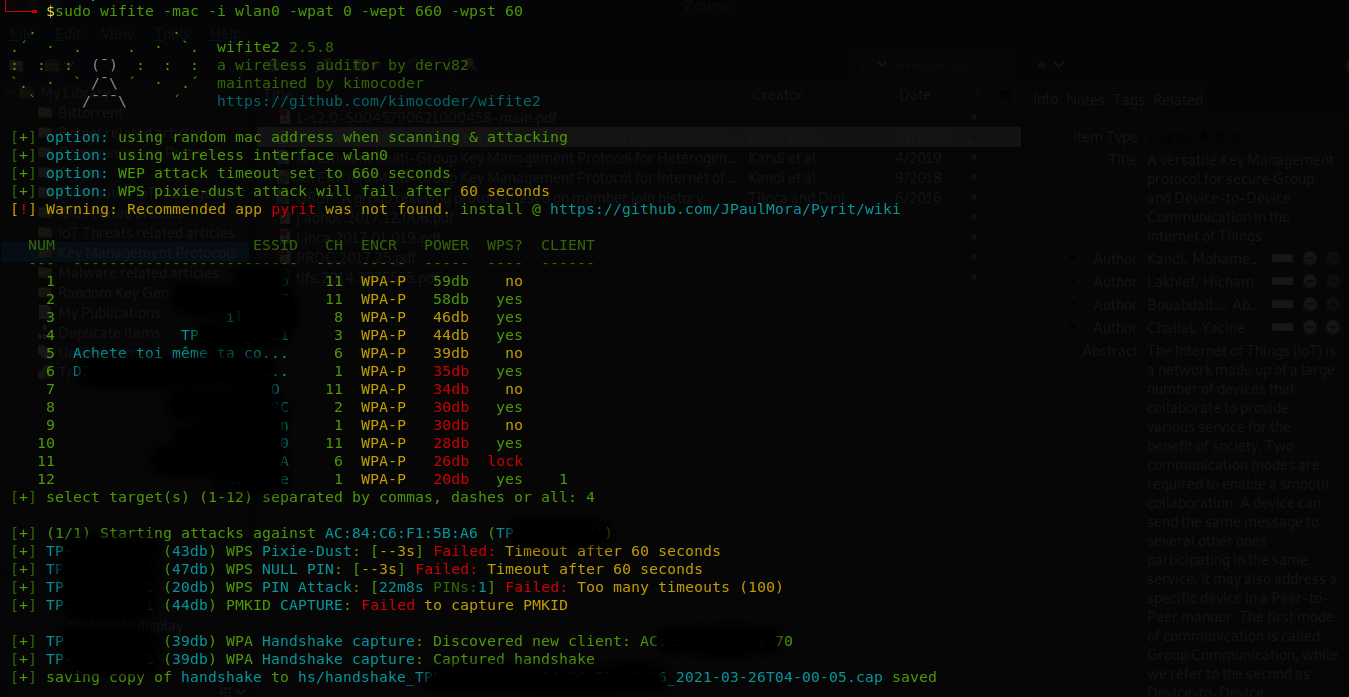
\includegraphics[scale=0.25]{figures/wifi/wifite1bis.png}}
	%\caption{Election procedure}
	\label{fig}
\end{figure}

The first step is to technically identify the WiFi AP through ots ESSID and BSSID. The objective is to dump a handshake exchange with one client. If we can manage to identify a connected client to the network, we can try to cut it off from thr network by sending multiple deauth frames. This will force the client to reconnect to the AP, allowing us to capture the handshake. Once the handshake is captured, we crack it to obtain the WiFi network’s key.

\begin{figure}[htbp]
	\centerline{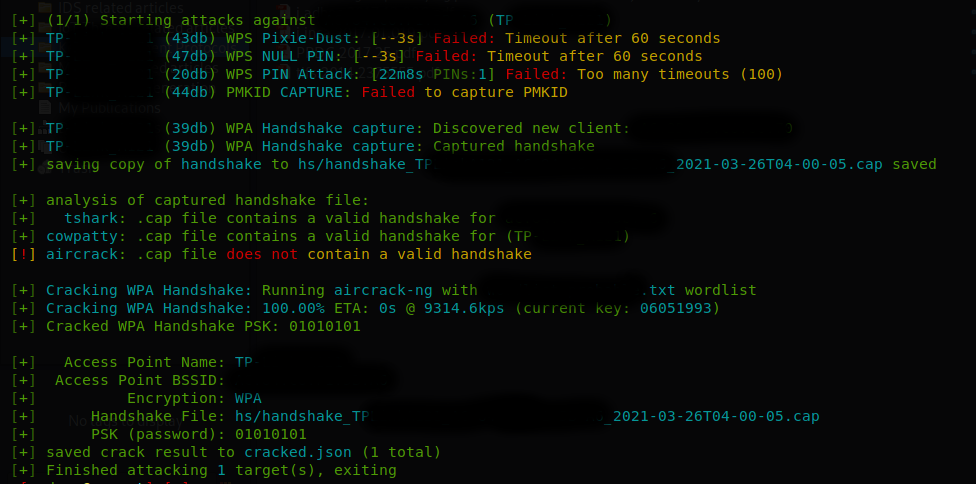
\includegraphics[scale=0.35]{figures/wifi/wifite2bis.png}}
	%\caption{Election procedure}
	\label{fig}
\end{figure}

What we actually do is that we analyse the captured .cap file to extract the password. We use a dictionary-based attack in order to find a match for the captured handshake by replaying the exchange for different possible passwords.

%\begin{figure}[htbp]
%	\centerline{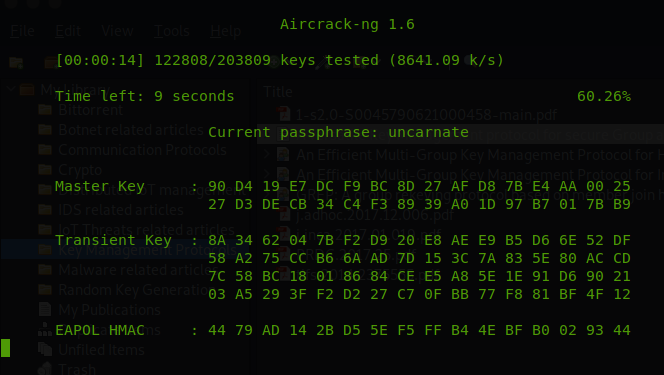
\includegraphics[scale=0.45]{figures/wifi/aircrack1.png}}
	%\caption{Election procedure}
%	\label{fig}
%\end{figure}

Using a dictionary-based password attack, we are able to recover the password in just few seconds.

\begin{figure}[htbp]
	\centerline{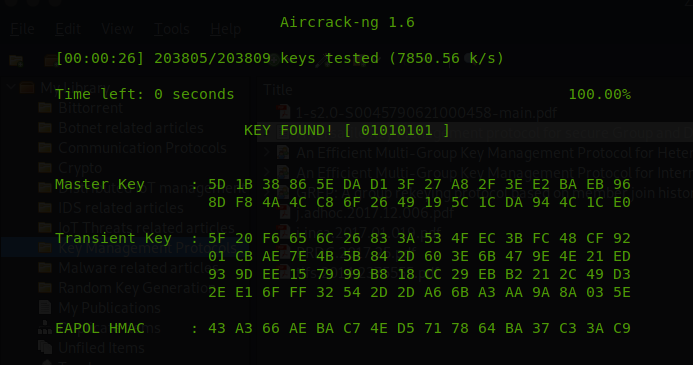
\includegraphics[scale=0.50]{figures/wifi/aircrack2.png}}
	%\caption{Election procedure}
	\label{fig}
\end{figure}
%\chapter{Bluetooth attack}

Dummy text.

\backmatter

%\bibliographystyle{ieeetr}
\bibliographystyle{plain}
\bibliography{refs}
%\bibliography{ch}
%\bibliography{communication.bib}
%\bibliography{crypto.bib}
%\bibliography{distributed_blockchain.bib}
%\bibliography{IDS.bib}
%\bibliography{iot_forensics.bib}
%\bibliography{key_management.bib}
%\bibliography{malware.bib}
%\bibliography{random_key_generation.bib}
%\bibliography{threats.bib}
%\bibliography{web}


%\includepdf[pages={-}]{declaration-originality.pdf}

\end{document}
